\documentclass[11pt]{article}

% Make this file compilable from the repo root or within `Lecture Tex/handouts/`.
\makeatletter
\def\input@path{{../../}{../}{Lecture Tex/}}
\makeatother
% Stat 221 LaTeX preamble (shared across lecture notes)

% --- Page + typography ---
\usepackage[margin=1in]{geometry}
\usepackage[T1]{fontenc}
\usepackage{libertinus}
\usepackage{libertinust1math}
\usepackage[scaled=0.95]{inconsolata}
\usepackage{microtype}

% --- Math + symbols ---
\usepackage{amsmath,amssymb,amsthm,mathtools}
\usepackage{bm}

% --- Layout helpers ---
\usepackage{graphicx}
\usepackage{booktabs}
\usepackage{enumitem}
\usepackage{titlesec}
\usepackage{fancyhdr}
\usepackage{xcolor}
\usepackage[most]{tcolorbox}
\usepackage{algorithm}
\usepackage{algpseudocode}

% --- Visual style ---
\definecolor{stat221Blue}{HTML}{1F4E79}
\definecolor{stat221BlueLight}{HTML}{EAF3FA}
\definecolor{stat221GrayLight}{HTML}{F6F7FB}
\definecolor{stat221Gray}{HTML}{2F2F2F}
\definecolor{stat221Purple}{HTML}{6A3D9A}
\definecolor{stat221PurpleLight}{HTML}{F3EEFA}
\definecolor{stat221Gold}{HTML}{9A6B00}
\definecolor{stat221GoldLight}{HTML}{FFF3D9}
\definecolor{stat221Teal}{HTML}{0F766E}
\definecolor{stat221TealLight}{HTML}{EAF7F6}
\definecolor{stat221Green}{HTML}{2E7D32}
\definecolor{stat221GreenLight}{HTML}{EDF8EF}
\definecolor{stat221Orange}{HTML}{B45309}
\definecolor{stat221OrangeLight}{HTML}{FFF4E8}
\definecolor{stat221Red}{HTML}{B2182B}
\colorlet{stat221TitleBack}{stat221Blue!12}

% --- Figures ---
\usepackage{tikz}
\usetikzlibrary{arrows.meta,calc,positioning,matrix}
\usepackage{pgfplots}
\pgfplotsset{compat=1.18}

% --- Bibliography ---
\usepackage[round]{natbib}

% --- Links and cross-references ---
\usepackage[colorlinks=true,linkcolor=stat221Blue,citecolor=stat221Blue,urlcolor=stat221Blue]{hyperref}
\usepackage[nameinlink,capitalise,noabbrev]{cleveref}

% Better names in references.
\crefname{algorithm}{Algorithm}{Algorithms}
\Crefname{algorithm}{Algorithm}{Algorithms}

% Refer to all sectioning levels uniformly as "Section".
\crefname{section}{Section}{Sections}
\Crefname{section}{Section}{Sections}
\crefname{subsection}{Section}{Sections}
\Crefname{subsection}{Section}{Sections}
\crefname{subsubsection}{Section}{Sections}
\Crefname{subsubsection}{Section}{Sections}

% Algorithmicx wording.
\algrenewcommand\algorithmicrequire{\textbf{Input:}}
\algrenewcommand\algorithmicensure{\textbf{Output:}}

% Avoid duplicate hyperref destinations for algorithmic line numbers.
\makeatletter
\providecommand{\theHALG@line}{}
\renewcommand{\theHALG@line}{ALG@line.\thealgorithm.\arabic{ALG@line}}
\makeatother

\setlength{\parindent}{0pt}
\setlength{\parskip}{0.5em}

\setlist[itemize]{leftmargin=*,topsep=0.25em,itemsep=0.15em}
\setlist[enumerate]{leftmargin=*,topsep=0.25em,itemsep=0.15em}

\titleformat{\section}{\Large\bfseries\color{stat221Blue}}{\thesection}{0.75em}{}
\titleformat{\subsection}{\large\bfseries\color{stat221Blue}}{\thesubsection}{0.75em}{}
\titleformat{\subsubsection}{\bfseries\color{stat221Gray}}{\thesubsubsection}{0.75em}{}
\titleformat{\part}[display]
  {\centering\Huge\bfseries\color{stat221Blue}}
  {}
  {0pt}
  {\vspace*{\fill}\partname~\thepart\\[0.6em]}
  [\vspace*{\fill}\thispagestyle{plain}\clearpage]
\titlespacing*{\part}{0pt}{0pt}{0pt}
\titlespacing*{\section}{0pt}{2.2ex plus 0.4ex minus 0.2ex}{1.0ex plus 0.2ex}
\titlespacing*{\subsection}{0pt}{1.6ex plus 0.3ex minus 0.2ex}{0.6ex plus 0.2ex}
\titlespacing*{\subsubsection}{0pt}{1.2ex plus 0.2ex minus 0.2ex}{0.3ex plus 0.2ex}

% Make parts full-page dividers: ensure `\part{...}` always starts a new page.
\let\statOrigPart\part
\renewcommand{\part}{\clearpage\statOrigPart}

% Keep the document structure uniform:
% - Show sections, subsections, and subsubsections in the table of contents.
\setcounter{secnumdepth}{3}
\setcounter{tocdepth}{3}

\pagestyle{fancy}
\fancyhf{}
\lhead{\textsc{Stat 221}}
\rhead{\nouppercase{\leftmark}}
\cfoot{\thepage}
\renewcommand{\headrulewidth}{0.4pt}
\setlength{\headheight}{14pt}
\fancypagestyle{plain}{
  \fancyhf{}
  \cfoot{\thepage}
  \renewcommand{\headrulewidth}{0pt}
}

% --- Theorem environments ---
\theoremstyle{definition}
\newtheorem{definition}{Definition}[section]
\newtheorem{example}[definition]{Example}
\newtheorem{exercise}[definition]{Exercise}

\theoremstyle{plain}
\newtheorem{theorem}[definition]{Theorem}
\newtheorem{proposition}[definition]{Proposition}
\newtheorem{lemma}[definition]{Lemma}
\newtheorem{corollary}[definition]{Corollary}

\theoremstyle{remark}
\newtheorem{remark}[definition]{Remark}

% --- Boxed theorem styling (keeps amsthm counters) ---
\tcbset{
  stat221box/.style={
    enhanced,
    breakable,
    lines before break=3,
    sharp corners,
    boxrule=0.6pt,
    coltitle=stat221Gray,
    fonttitle=\bfseries,
    left=8pt,right=8pt,top=6pt,bottom=6pt,
  },
  stat221titlebox/.style={
    stat221box,
    colbacktitle=stat221TitleBack,
    boxed title style={colback=stat221TitleBack,colframe=stat221Blue!60!black},
  },
  stat221panelblue/.style={
    stat221titlebox,
    colback=stat221BlueLight,
    colframe=stat221Blue!60!black,
  },
  stat221panelgray/.style={
    stat221titlebox,
    colback=stat221GrayLight,
    colframe=stat221Blue!60!black,
  },
}

\tcolorboxenvironment{definition}{stat221box,colback=stat221BlueLight,colframe=stat221Blue!60!black}
\tcolorboxenvironment{example}{stat221box,colback=stat221GoldLight,colframe=stat221Gold!70!black}
\tcolorboxenvironment{exercise}{stat221box,colback=stat221OrangeLight,colframe=stat221Orange!70!black}
\tcolorboxenvironment{theorem}{stat221box,colback=stat221GrayLight,colframe=stat221Gray!70!black}
\tcolorboxenvironment{lemma}{stat221box,colback=stat221GreenLight,colframe=stat221Green!60!black}
\tcolorboxenvironment{proposition}{stat221box,colback=stat221PurpleLight,colframe=stat221Purple!60!black}
\tcolorboxenvironment{corollary}{stat221box,colback=stat221TealLight,colframe=stat221Teal!60!black}
\tcolorboxenvironment{remark}{stat221box,colback=white,colframe=stat221Gray!50!black}

\renewcommand{\qedsymbol}{$\blacksquare$}

% --- Macros ---
\newcommand{\R}{\mathbb{R}}
\newcommand{\C}{\mathbb{C}}
\newcommand{\E}{\mathbb{E}}
\newcommand{\1}{\mathbf{1}}

\DeclareMathOperator*{\argmin}{arg\,min}
\DeclareMathOperator*{\argmax}{arg\,max}

\DeclarePairedDelimiter\norm{\lVert}{\rVert}
\DeclarePairedDelimiter\ip{\langle}{\rangle}

% A consistent Hessian notation (to avoid ambiguity with other uses of \nabla^2).
\newcommand{\Hess}{\nabla^2}

\usepackage{float} % for [H] placement specifier in algorithms

\graphicspath{{../../}{../}{Lecture Tex/}{../../figures/}{../figures/}{Lecture Tex/figures/}}

% ------------------------------------------------------------
% Build toggle for solutions.
% - Student version (default): show workspace boxes, hide solutions.
% - Solutions version: define \STATshowsolutions on the command line.
%   Preferred repo-level build (compiles the titled PDFs directly and clears legacy outputs):
%     python3 scripts/build_handouts.py --section 4
%   Example:
%     pdflatex "\def\STATshowsolutions{1}\documentclass[11pt]{article}

% Make this file compilable from the repo root or within `Lecture Tex/handouts/`.
\makeatletter
\def\input@path{{../../}{../}{Lecture Tex/}}
\makeatother
% Stat 221 LaTeX preamble (shared across lecture notes)

% --- Page + typography ---
\usepackage[margin=1in]{geometry}
\usepackage[T1]{fontenc}
\usepackage{libertinus}
\usepackage{libertinust1math}
\usepackage[scaled=0.95]{inconsolata}
\usepackage{microtype}

% --- Math + symbols ---
\usepackage{amsmath,amssymb,amsthm,mathtools}
\usepackage{bm}

% --- Layout helpers ---
\usepackage{graphicx}
\usepackage{booktabs}
\usepackage{enumitem}
\usepackage{titlesec}
\usepackage{fancyhdr}
\usepackage{xcolor}
\usepackage[most]{tcolorbox}
\usepackage{algorithm}
\usepackage{algpseudocode}

% --- Visual style ---
\definecolor{stat221Blue}{HTML}{1F4E79}
\definecolor{stat221BlueLight}{HTML}{EAF3FA}
\definecolor{stat221GrayLight}{HTML}{F6F7FB}
\definecolor{stat221Gray}{HTML}{2F2F2F}
\definecolor{stat221Purple}{HTML}{6A3D9A}
\definecolor{stat221PurpleLight}{HTML}{F3EEFA}
\definecolor{stat221Gold}{HTML}{9A6B00}
\definecolor{stat221GoldLight}{HTML}{FFF3D9}
\definecolor{stat221Teal}{HTML}{0F766E}
\definecolor{stat221TealLight}{HTML}{EAF7F6}
\definecolor{stat221Green}{HTML}{2E7D32}
\definecolor{stat221GreenLight}{HTML}{EDF8EF}
\definecolor{stat221Orange}{HTML}{B45309}
\definecolor{stat221OrangeLight}{HTML}{FFF4E8}
\definecolor{stat221Red}{HTML}{B2182B}
\colorlet{stat221TitleBack}{stat221Blue!12}

% --- Figures ---
\usepackage{tikz}
\usetikzlibrary{arrows.meta,calc,positioning,matrix}
\usepackage{pgfplots}
\pgfplotsset{compat=1.18}

% --- Bibliography ---
\usepackage[round]{natbib}

% --- Links and cross-references ---
\usepackage[colorlinks=true,linkcolor=stat221Blue,citecolor=stat221Blue,urlcolor=stat221Blue]{hyperref}
\usepackage[nameinlink,capitalise,noabbrev]{cleveref}

% Better names in references.
\crefname{algorithm}{Algorithm}{Algorithms}
\Crefname{algorithm}{Algorithm}{Algorithms}

% Refer to all sectioning levels uniformly as "Section".
\crefname{section}{Section}{Sections}
\Crefname{section}{Section}{Sections}
\crefname{subsection}{Section}{Sections}
\Crefname{subsection}{Section}{Sections}
\crefname{subsubsection}{Section}{Sections}
\Crefname{subsubsection}{Section}{Sections}

% Algorithmicx wording.
\algrenewcommand\algorithmicrequire{\textbf{Input:}}
\algrenewcommand\algorithmicensure{\textbf{Output:}}

% Avoid duplicate hyperref destinations for algorithmic line numbers.
\makeatletter
\providecommand{\theHALG@line}{}
\renewcommand{\theHALG@line}{ALG@line.\thealgorithm.\arabic{ALG@line}}
\makeatother

\setlength{\parindent}{0pt}
\setlength{\parskip}{0.5em}

\setlist[itemize]{leftmargin=*,topsep=0.25em,itemsep=0.15em}
\setlist[enumerate]{leftmargin=*,topsep=0.25em,itemsep=0.15em}

\titleformat{\section}{\Large\bfseries\color{stat221Blue}}{\thesection}{0.75em}{}
\titleformat{\subsection}{\large\bfseries\color{stat221Blue}}{\thesubsection}{0.75em}{}
\titleformat{\subsubsection}{\bfseries\color{stat221Gray}}{\thesubsubsection}{0.75em}{}
\titleformat{\part}[display]
  {\centering\Huge\bfseries\color{stat221Blue}}
  {}
  {0pt}
  {\vspace*{\fill}\partname~\thepart\\[0.6em]}
  [\vspace*{\fill}\thispagestyle{plain}\clearpage]
\titlespacing*{\part}{0pt}{0pt}{0pt}
\titlespacing*{\section}{0pt}{2.2ex plus 0.4ex minus 0.2ex}{1.0ex plus 0.2ex}
\titlespacing*{\subsection}{0pt}{1.6ex plus 0.3ex minus 0.2ex}{0.6ex plus 0.2ex}
\titlespacing*{\subsubsection}{0pt}{1.2ex plus 0.2ex minus 0.2ex}{0.3ex plus 0.2ex}

% Make parts full-page dividers: ensure `\part{...}` always starts a new page.
\let\statOrigPart\part
\renewcommand{\part}{\clearpage\statOrigPart}

% Keep the document structure uniform:
% - Show sections, subsections, and subsubsections in the table of contents.
\setcounter{secnumdepth}{3}
\setcounter{tocdepth}{3}

\pagestyle{fancy}
\fancyhf{}
\lhead{\textsc{Stat 221}}
\rhead{\nouppercase{\leftmark}}
\cfoot{\thepage}
\renewcommand{\headrulewidth}{0.4pt}
\setlength{\headheight}{14pt}
\fancypagestyle{plain}{
  \fancyhf{}
  \cfoot{\thepage}
  \renewcommand{\headrulewidth}{0pt}
}

% --- Theorem environments ---
\theoremstyle{definition}
\newtheorem{definition}{Definition}[section]
\newtheorem{example}[definition]{Example}
\newtheorem{exercise}[definition]{Exercise}

\theoremstyle{plain}
\newtheorem{theorem}[definition]{Theorem}
\newtheorem{proposition}[definition]{Proposition}
\newtheorem{lemma}[definition]{Lemma}
\newtheorem{corollary}[definition]{Corollary}

\theoremstyle{remark}
\newtheorem{remark}[definition]{Remark}

% --- Boxed theorem styling (keeps amsthm counters) ---
\tcbset{
  stat221box/.style={
    enhanced,
    breakable,
    lines before break=3,
    sharp corners,
    boxrule=0.6pt,
    coltitle=stat221Gray,
    fonttitle=\bfseries,
    left=8pt,right=8pt,top=6pt,bottom=6pt,
  },
  stat221titlebox/.style={
    stat221box,
    colbacktitle=stat221TitleBack,
    boxed title style={colback=stat221TitleBack,colframe=stat221Blue!60!black},
  },
  stat221panelblue/.style={
    stat221titlebox,
    colback=stat221BlueLight,
    colframe=stat221Blue!60!black,
  },
  stat221panelgray/.style={
    stat221titlebox,
    colback=stat221GrayLight,
    colframe=stat221Blue!60!black,
  },
}

\tcolorboxenvironment{definition}{stat221box,colback=stat221BlueLight,colframe=stat221Blue!60!black}
\tcolorboxenvironment{example}{stat221box,colback=stat221GoldLight,colframe=stat221Gold!70!black}
\tcolorboxenvironment{exercise}{stat221box,colback=stat221OrangeLight,colframe=stat221Orange!70!black}
\tcolorboxenvironment{theorem}{stat221box,colback=stat221GrayLight,colframe=stat221Gray!70!black}
\tcolorboxenvironment{lemma}{stat221box,colback=stat221GreenLight,colframe=stat221Green!60!black}
\tcolorboxenvironment{proposition}{stat221box,colback=stat221PurpleLight,colframe=stat221Purple!60!black}
\tcolorboxenvironment{corollary}{stat221box,colback=stat221TealLight,colframe=stat221Teal!60!black}
\tcolorboxenvironment{remark}{stat221box,colback=white,colframe=stat221Gray!50!black}

\renewcommand{\qedsymbol}{$\blacksquare$}

% --- Macros ---
\newcommand{\R}{\mathbb{R}}
\newcommand{\C}{\mathbb{C}}
\newcommand{\E}{\mathbb{E}}
\newcommand{\1}{\mathbf{1}}

\DeclareMathOperator*{\argmin}{arg\,min}
\DeclareMathOperator*{\argmax}{arg\,max}

\DeclarePairedDelimiter\norm{\lVert}{\rVert}
\DeclarePairedDelimiter\ip{\langle}{\rangle}

% A consistent Hessian notation (to avoid ambiguity with other uses of \nabla^2).
\newcommand{\Hess}{\nabla^2}

\usepackage{float} % for [H] placement specifier in algorithms

\graphicspath{{../../}{../}{Lecture Tex/}{../../figures/}{../figures/}{Lecture Tex/figures/}}

% ------------------------------------------------------------
% Build toggle for solutions.
% - Student version (default): show workspace boxes, hide solutions.
% - Solutions version: define \STATshowsolutions on the command line.
%   Preferred repo-level build (compiles the titled PDFs directly and clears legacy outputs):
%     python3 scripts/build_handouts.py --section 4
%   Example:
%     pdflatex "\def\STATshowsolutions{1}\documentclass[11pt]{article}

% Make this file compilable from the repo root or within `Lecture Tex/handouts/`.
\makeatletter
\def\input@path{{../../}{../}{Lecture Tex/}}
\makeatother
% Stat 221 LaTeX preamble (shared across lecture notes)

% --- Page + typography ---
\usepackage[margin=1in]{geometry}
\usepackage[T1]{fontenc}
\usepackage{libertinus}
\usepackage{libertinust1math}
\usepackage[scaled=0.95]{inconsolata}
\usepackage{microtype}

% --- Math + symbols ---
\usepackage{amsmath,amssymb,amsthm,mathtools}
\usepackage{bm}

% --- Layout helpers ---
\usepackage{graphicx}
\usepackage{booktabs}
\usepackage{enumitem}
\usepackage{titlesec}
\usepackage{fancyhdr}
\usepackage{xcolor}
\usepackage[most]{tcolorbox}
\usepackage{algorithm}
\usepackage{algpseudocode}

% --- Visual style ---
\definecolor{stat221Blue}{HTML}{1F4E79}
\definecolor{stat221BlueLight}{HTML}{EAF3FA}
\definecolor{stat221GrayLight}{HTML}{F6F7FB}
\definecolor{stat221Gray}{HTML}{2F2F2F}
\definecolor{stat221Purple}{HTML}{6A3D9A}
\definecolor{stat221PurpleLight}{HTML}{F3EEFA}
\definecolor{stat221Gold}{HTML}{9A6B00}
\definecolor{stat221GoldLight}{HTML}{FFF3D9}
\definecolor{stat221Teal}{HTML}{0F766E}
\definecolor{stat221TealLight}{HTML}{EAF7F6}
\definecolor{stat221Green}{HTML}{2E7D32}
\definecolor{stat221GreenLight}{HTML}{EDF8EF}
\definecolor{stat221Orange}{HTML}{B45309}
\definecolor{stat221OrangeLight}{HTML}{FFF4E8}
\definecolor{stat221Red}{HTML}{B2182B}
\colorlet{stat221TitleBack}{stat221Blue!12}

% --- Figures ---
\usepackage{tikz}
\usetikzlibrary{arrows.meta,calc,positioning,matrix}
\usepackage{pgfplots}
\pgfplotsset{compat=1.18}

% --- Bibliography ---
\usepackage[round]{natbib}

% --- Links and cross-references ---
\usepackage[colorlinks=true,linkcolor=stat221Blue,citecolor=stat221Blue,urlcolor=stat221Blue]{hyperref}
\usepackage[nameinlink,capitalise,noabbrev]{cleveref}

% Better names in references.
\crefname{algorithm}{Algorithm}{Algorithms}
\Crefname{algorithm}{Algorithm}{Algorithms}

% Refer to all sectioning levels uniformly as "Section".
\crefname{section}{Section}{Sections}
\Crefname{section}{Section}{Sections}
\crefname{subsection}{Section}{Sections}
\Crefname{subsection}{Section}{Sections}
\crefname{subsubsection}{Section}{Sections}
\Crefname{subsubsection}{Section}{Sections}

% Algorithmicx wording.
\algrenewcommand\algorithmicrequire{\textbf{Input:}}
\algrenewcommand\algorithmicensure{\textbf{Output:}}

% Avoid duplicate hyperref destinations for algorithmic line numbers.
\makeatletter
\providecommand{\theHALG@line}{}
\renewcommand{\theHALG@line}{ALG@line.\thealgorithm.\arabic{ALG@line}}
\makeatother

\setlength{\parindent}{0pt}
\setlength{\parskip}{0.5em}

\setlist[itemize]{leftmargin=*,topsep=0.25em,itemsep=0.15em}
\setlist[enumerate]{leftmargin=*,topsep=0.25em,itemsep=0.15em}

\titleformat{\section}{\Large\bfseries\color{stat221Blue}}{\thesection}{0.75em}{}
\titleformat{\subsection}{\large\bfseries\color{stat221Blue}}{\thesubsection}{0.75em}{}
\titleformat{\subsubsection}{\bfseries\color{stat221Gray}}{\thesubsubsection}{0.75em}{}
\titleformat{\part}[display]
  {\centering\Huge\bfseries\color{stat221Blue}}
  {}
  {0pt}
  {\vspace*{\fill}\partname~\thepart\\[0.6em]}
  [\vspace*{\fill}\thispagestyle{plain}\clearpage]
\titlespacing*{\part}{0pt}{0pt}{0pt}
\titlespacing*{\section}{0pt}{2.2ex plus 0.4ex minus 0.2ex}{1.0ex plus 0.2ex}
\titlespacing*{\subsection}{0pt}{1.6ex plus 0.3ex minus 0.2ex}{0.6ex plus 0.2ex}
\titlespacing*{\subsubsection}{0pt}{1.2ex plus 0.2ex minus 0.2ex}{0.3ex plus 0.2ex}

% Make parts full-page dividers: ensure `\part{...}` always starts a new page.
\let\statOrigPart\part
\renewcommand{\part}{\clearpage\statOrigPart}

% Keep the document structure uniform:
% - Show sections, subsections, and subsubsections in the table of contents.
\setcounter{secnumdepth}{3}
\setcounter{tocdepth}{3}

\pagestyle{fancy}
\fancyhf{}
\lhead{\textsc{Stat 221}}
\rhead{\nouppercase{\leftmark}}
\cfoot{\thepage}
\renewcommand{\headrulewidth}{0.4pt}
\setlength{\headheight}{14pt}
\fancypagestyle{plain}{
  \fancyhf{}
  \cfoot{\thepage}
  \renewcommand{\headrulewidth}{0pt}
}

% --- Theorem environments ---
\theoremstyle{definition}
\newtheorem{definition}{Definition}[section]
\newtheorem{example}[definition]{Example}
\newtheorem{exercise}[definition]{Exercise}

\theoremstyle{plain}
\newtheorem{theorem}[definition]{Theorem}
\newtheorem{proposition}[definition]{Proposition}
\newtheorem{lemma}[definition]{Lemma}
\newtheorem{corollary}[definition]{Corollary}

\theoremstyle{remark}
\newtheorem{remark}[definition]{Remark}

% --- Boxed theorem styling (keeps amsthm counters) ---
\tcbset{
  stat221box/.style={
    enhanced,
    breakable,
    lines before break=3,
    sharp corners,
    boxrule=0.6pt,
    coltitle=stat221Gray,
    fonttitle=\bfseries,
    left=8pt,right=8pt,top=6pt,bottom=6pt,
  },
  stat221titlebox/.style={
    stat221box,
    colbacktitle=stat221TitleBack,
    boxed title style={colback=stat221TitleBack,colframe=stat221Blue!60!black},
  },
  stat221panelblue/.style={
    stat221titlebox,
    colback=stat221BlueLight,
    colframe=stat221Blue!60!black,
  },
  stat221panelgray/.style={
    stat221titlebox,
    colback=stat221GrayLight,
    colframe=stat221Blue!60!black,
  },
}

\tcolorboxenvironment{definition}{stat221box,colback=stat221BlueLight,colframe=stat221Blue!60!black}
\tcolorboxenvironment{example}{stat221box,colback=stat221GoldLight,colframe=stat221Gold!70!black}
\tcolorboxenvironment{exercise}{stat221box,colback=stat221OrangeLight,colframe=stat221Orange!70!black}
\tcolorboxenvironment{theorem}{stat221box,colback=stat221GrayLight,colframe=stat221Gray!70!black}
\tcolorboxenvironment{lemma}{stat221box,colback=stat221GreenLight,colframe=stat221Green!60!black}
\tcolorboxenvironment{proposition}{stat221box,colback=stat221PurpleLight,colframe=stat221Purple!60!black}
\tcolorboxenvironment{corollary}{stat221box,colback=stat221TealLight,colframe=stat221Teal!60!black}
\tcolorboxenvironment{remark}{stat221box,colback=white,colframe=stat221Gray!50!black}

\renewcommand{\qedsymbol}{$\blacksquare$}

% --- Macros ---
\newcommand{\R}{\mathbb{R}}
\newcommand{\C}{\mathbb{C}}
\newcommand{\E}{\mathbb{E}}
\newcommand{\1}{\mathbf{1}}

\DeclareMathOperator*{\argmin}{arg\,min}
\DeclareMathOperator*{\argmax}{arg\,max}

\DeclarePairedDelimiter\norm{\lVert}{\rVert}
\DeclarePairedDelimiter\ip{\langle}{\rangle}

% A consistent Hessian notation (to avoid ambiguity with other uses of \nabla^2).
\newcommand{\Hess}{\nabla^2}

\usepackage{float} % for [H] placement specifier in algorithms

\graphicspath{{../../}{../}{Lecture Tex/}{../../figures/}{../figures/}{Lecture Tex/figures/}}

% ------------------------------------------------------------
% Build toggle for solutions.
% - Student version (default): show workspace boxes, hide solutions.
% - Solutions version: define \STATshowsolutions on the command line.
%   Preferred repo-level build (compiles the titled PDFs directly and clears legacy outputs):
%     python3 scripts/build_handouts.py --section 4
%   Example:
%     pdflatex "\def\STATshowsolutions{1}\documentclass[11pt]{article}

% Make this file compilable from the repo root or within `Lecture Tex/handouts/`.
\makeatletter
\def\input@path{{../../}{../}{Lecture Tex/}}
\makeatother
\input{preamble}
\usepackage{float} % for [H] placement specifier in algorithms

\graphicspath{{../../}{../}{Lecture Tex/}{../../figures/}{../figures/}{Lecture Tex/figures/}}

% ------------------------------------------------------------
% Build toggle for solutions.
% - Student version (default): show workspace boxes, hide solutions.
% - Solutions version: define \STATshowsolutions on the command line.
%   Preferred repo-level build (compiles the titled PDFs directly and clears legacy outputs):
%     python3 scripts/build_handouts.py --section 4
%   Example:
%     pdflatex "\def\STATshowsolutions{1}\input{Lecture Tex/handouts/section 4/section_hmc_geometry.tex}"
%   (Low-level direct build: if you invoke latexmk manually, set -jobname to the
%    titled output so the compiled PDF matches the standard naming scheme.)
\newif\ifshowsolutions
\showsolutionsfalse
\ifdefined\STATshowsolutions
  \showsolutionstrue
\fi
\ifcsname STAT221SOLUTIONS\endcsname
  \showsolutionstrue
\fi

% Solutions/workspace boxes (controlled by \ifshowsolutions).
% Usage: \SolutionBox[<workspace lines>]{<solution body>}
\newcommand{\SolutionBox}[2][10]{%
  \ifshowsolutions
    \begin{tcolorbox}[stat221panelgray,title={Solution}]
    #2
    \end{tcolorbox}
  \else
    \begin{tcolorbox}[stat221panelgray,unbreakable,title={Workspace}]
    \vspace{#1\baselineskip}
    \end{tcolorbox}
  \fi
}

\title{How do entropy and transport control Langevin convergence?}
\author{}
\date{}

\begin{document}
\maketitle

\section[Entropy, transport, and Langevin]{How do entropy and transport control Langevin convergence?}
\label{sec:langevin-handout-opening}

This handout takes one question from the Sampling unit and studies it in continuous time: how fast does the overdamped Langevin law approach equilibrium, and which geometric assumptions control that rate?
The diffusion itself is
\[
dX_t=-\nabla U(X_t)\,dt+\sqrt{2}\,dB_t,
\]
with stationary law
\[
\pi(x)=Z^{-1}e^{-U(x)}.
\]
Here $Z=\int_{\R^d} e^{-U(x)}\,dx$ is assumed finite, and the evolving object is the law $\rho_t=\mathcal{L}(X_t)$ when $X_0$ does not start from equilibrium.
The main quantities will be the free-energy gap, its dissipation along the Langevin flow, and the transport inequalities that turn dissipation into quantitative convergence.

This viewpoint extends the Sampling unit's gradient-based MCMC subsection, reuses the Optimization unit's language of objectives, proximal structure, and conditioning in measure space, and feeds directly into the Augmented-state sampling unit.
There the same local geometry drives HMC and NUTS through momentum-carrying trajectories rather than one-step Langevin corrections.

There is also a concrete geometric reason to care.
For a quadratic target
\[
U(x)=\frac12 x^\top Hx,
\]
every mode in an eigenbasis of $H$ relaxes at its own exponential rate.
If $H$ is poorly conditioned, then one slow direction controls the last stage of convergence even when the other directions have already equilibrated.
So even in the friendliest Gaussian case, convergence is already controlled by geometry.
The rest of the note develops the general version of that picture:
we identify a free-energy gap to equilibrium, compute its dissipation along the Langevin flow, convert that dissipation into explicit entropy and transport rates, and then read off how preconditioning changes the governing matrix in quadratic and locally quadratic models.

Throughout we work in the smooth, rapidly decaying setting when we differentiate under the integral sign or integrate by parts.
Those formal calculations are the right ones, and the cited theorems extend them to broader classes of densities.

\section{A notion of distance to equilibrium}
\label{sec:free-energy-fokker-planck}

The first task is to identify the right notion of distance to equilibrium.
For Langevin, the natural candidate is not Euclidean distance between points but a functional on densities.
The standard object here is the free-energy gap, and the corresponding density evolution is governed by the Fokker--Planck equation.

\subsection{Relative entropy is a free-energy gap}
\label{subsec:free-energy-gap}

Fix a potential $U:\R^d\to\R$ and define the target density
\[
\pi(x)=Z^{-1}e^{-U(x)},
\qquad
Z=\int_{\R^d} e^{-U(x)}\,dx.
\]
For a probability density $\rho$ we define the free energy
\begin{equation}
  \mathcal{F}(\rho)
  :=
  \int_{\R^d} U(x)\rho(x)\,dx
  +
  \int_{\R^d} \rho(x)\log \rho(x)\,dx.
  \label{eq:free-energy-definition}
\end{equation}
The first term is potential energy.
The second is minus the Shannon entropy, so $\mathcal{F}$ is the natural energy--entropy tradeoff for Langevin diffusion.

\begin{proposition}[Relative entropy equals the free-energy gap]
\label{prop:free-energy-kl}
For every probability density $\rho$ with finite free energy,
\begin{equation}
  D_{\mathrm{KL}}(\rho\|\pi)
  =
  \mathcal{F}(\rho)-\mathcal{F}(\pi).
  \label{eq:free-energy-gap}
\end{equation}
In particular,
\[
\mathcal{F}(\pi)=-\log Z,
\]
so minimizing free energy is the same as minimizing relative entropy to $\pi$.
\end{proposition}

\begin{proof}
Since $\log \pi(x)=-U(x)-\log Z$,
\begin{align*}
  D_{\mathrm{KL}}(\rho\|\pi)
  &=
  \int \rho(x)\log\frac{\rho(x)}{\pi(x)}\,dx \\
  &=
  \int \rho(x)\log \rho(x)\,dx
  +
  \int U(x)\rho(x)\,dx
  +
  \log Z \\
  &=
  \mathcal{F}(\rho)+\log Z.
\end{align*}
Applying the same identity with $\rho=\pi$ gives
\[
0=D_{\mathrm{KL}}(\pi\|\pi)=\mathcal{F}(\pi)+\log Z,
\]
so $\mathcal{F}(\pi)=-\log Z$.
Substituting this into the first formula yields \eqref{eq:free-energy-gap}.%
\end{proof}

\Cref{prop:free-energy-kl} is the basic dictionary for the rest of the note.
The object that decreases along Langevin is not an ad hoc Lyapunov function.
It is exactly the distance to equilibrium measured in relative entropy.

\begin{exercise}[Deriving the free-energy identity]
\label{ex:free-energy-gap}
Starting from \Cref{eq:free-energy-definition} and $\pi(x)=Z^{-1}e^{-U(x)}$, derive \Cref{eq:free-energy-gap}.
Then show directly that $\pi$ minimizes $\mathcal{F}$ over all densities.
\end{exercise}
\SolutionBox[12]{%
We expand the logarithm of the target:
\[
\log \pi(x)=-U(x)-\log Z.
\]
Therefore
\begin{align*}
  D_{\mathrm{KL}}(\rho\|\pi)
  &=
  \int \rho(x)\log\frac{\rho(x)}{\pi(x)}\,dx \\
  &=
  \int \rho(x)\log \rho(x)\,dx
  +
  \int U(x)\rho(x)\,dx
  +
  \log Z \\
  &=
  \mathcal{F}(\rho)+\log Z.
\end{align*}
Setting $\rho=\pi$ gives
\[
0=D_{\mathrm{KL}}(\pi\|\pi)=\mathcal{F}(\pi)+\log Z,
\]
so $\mathcal{F}(\pi)=-\log Z$, hence
\[
D_{\mathrm{KL}}(\rho\|\pi)=\mathcal{F}(\rho)-\mathcal{F}(\pi).
\]
Because relative entropy is always nonnegative and vanishes only when $\rho=\pi$ almost everywhere, $\pi$ is the unique minimizer of $\mathcal{F}$.%
}

\subsection{Langevin as a continuity equation}
\label{subsec:fokker-planck-continuity}

The overdamped Langevin diffusion is
\begin{equation}
  dX_t=-\nabla U(X_t)\,dt+\sqrt{2}\,dB_t.
  \label{eq:overdamped-langevin}
\end{equation}
If $\rho_t$ denotes the density of $X_t$, then $\rho_t$ solves the Fokker--Planck equation
\begin{equation}
  \partial_t \rho_t
  =
  \nabla\cdot(\rho_t\nabla U)+\Delta \rho_t.
  \label{eq:fokker-planck-basic}
\end{equation}
The key rewrite is that the diffusion term can be absorbed into the logarithmic derivative of $\rho_t$.

\begin{proposition}[Continuity-equation form of Fokker--Planck]
\label{prop:fokker-planck-continuity}
Assume $\rho_t$ is smooth and strictly positive.
Then \eqref{eq:fokker-planck-basic} can be written as
\begin{equation}
  \partial_t \rho_t
  =
  \nabla\cdot\!\bigl(\rho_t \nabla(U+\log\rho_t)\bigr)
  =
  -\nabla\cdot(\rho_t v_t),
  \label{eq:fokker-planck-continuity}
\end{equation}
with velocity field
\begin{equation}
  v_t
  =
  -\nabla\bigl(U+\log\rho_t\bigr).
  \label{eq:fokker-planck-velocity}
\end{equation}
\end{proposition}

\begin{proof}
Because $\rho_t>0$,
\[
\Delta \rho_t
=
\nabla\cdot(\nabla \rho_t)
=
\nabla\cdot\!\bigl(\rho_t\nabla\log\rho_t\bigr).
\]
Substituting this into \eqref{eq:fokker-planck-basic} gives
\[
\partial_t \rho_t
=
\nabla\cdot\!\bigl(\rho_t\nabla U\bigr)
+
\nabla\cdot\!\bigl(\rho_t\nabla\log\rho_t\bigr)
=
\nabla\cdot\!\bigl(\rho_t\nabla(U+\log\rho_t)\bigr).
\]
Defining $v_t$ by \eqref{eq:fokker-planck-velocity} yields the continuity equation in \eqref{eq:fokker-planck-continuity}.%
\end{proof}

The field $U+\log \rho_t$ is the first variation of free energy, up to an irrelevant additive constant.
So \Cref{prop:fokker-planck-continuity} says that mass moves downhill in free energy.
What it does not yet give is a one-step rule.
If we freeze time and ask which nearby density should count as the next descent step, we need to say how expensive it is to move one probability law to another.
That is the role of the JKO scheme.

\section{A variational one-step descent rule}
\label{sec:jko}

Free energy tells us what should decrease, but we still need a rule for how to choose the next density from the current one.
Starting from $\rho_k$, we want a new law that lowers $\mathcal{F}$ without moving mass arbitrarily far in a single step.
The Jordan--Kinderlehrer--Otto (JKO) construction is the variational rule that makes that tradeoff precise.

The analogy from Euclidean optimization is the proximal form of implicit Euler.
For the ODE $\dot x=-\nabla F(x)$,
\[
x_{k+1}\in\argmin_x \frac{1}{2h}\norm{x-x_k}_2^2+F(x).
\]
The JKO step does the same thing for densities.
It replaces the Euclidean quadratic penalty by a transport penalty between probability measures.
This is the point where the optimization and sampling viewpoints literally meet.
The same implicit-step logic used to stabilize descent methods in optimization becomes a rule for evolving \emph{laws} in sampling, with Wasserstein distance replacing Euclidean distance and free energy replacing the objective function.

\begin{figure}[t]
  \centering
  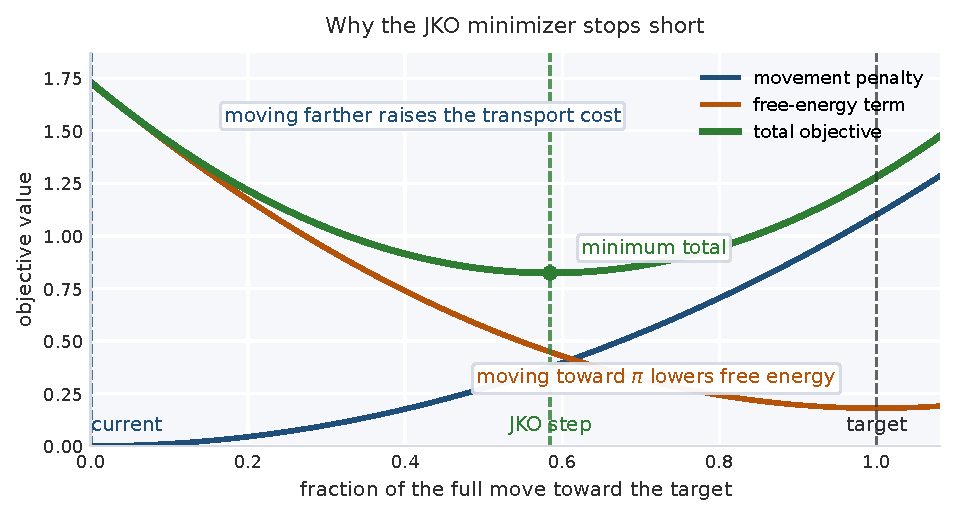
\includegraphics[width=0.9\linewidth]{figures/handouts/langevin_entropy_transport/fig_jko_tradeoff}
  \caption{One JKO step balances two competing effects.
  Moving farther toward equilibrium lowers the free-energy term, but it also increases the Wasserstein movement penalty, so the minimizer of the total objective stops at an interior compromise rather than jumping all the way to $\pi$.}
  \label{fig:jko-tradeoff}
\end{figure}

For a time step $h>0$, the JKO update is
\begin{equation}
  \rho_{k+1}
  \in
  \argmin_{\rho\in\mathcal{P}_2(\R^d)}
  \left\{
    \frac{1}{2h}W_2^2(\rho,\rho_k)+\mathcal{F}(\rho)
  \right\}.
  \label{eq:jko-step}
\end{equation}
The first term penalizes moving too far from the current density.
The second rewards lower free energy.
\Cref{fig:jko-tradeoff} is the picture to keep in mind: JKO is not ``jump to the minimizer of $\mathcal{F}$''; it is a one-step compromise between transport cost and dissipation.

\subsection{A Gaussian JKO calculation}
\label{subsec:jko-gaussian}

Take a quadratic target
\[
U(x)=\frac12 x^\top Hx,
\qquad
H\succ 0,
\]
so the equilibrium law is $\pi=\mathcal{N}(0,H^{-1})$.
To see what \eqref{eq:jko-step} is doing, first restrict attention to the translated Gaussian family
\[
\rho_m:=\mathcal{N}(m,H^{-1}),
\qquad
m\in\R^d.
\]
The covariance already matches the target, so only the mean is moving.

\begin{proposition}[Gaussian JKO mean update]
\label{prop:gaussian-jko-mean}
Fix $m_k\in\R^d$ and let $\rho_k=\rho_{m_k}$.
If we minimize the JKO objective \eqref{eq:jko-step} over translated Gaussians $\rho_m$, then
\begin{equation}
  m_{k+1}
  =
  (I_d+hH)^{-1}m_k.
  \label{eq:gaussian-jko-mean}
\end{equation}
Equivalently, the mean follows implicit Euler for the ODE $\dot m=-Hm$.
\end{proposition}

\begin{proof}
All densities $\rho_m$ have the same covariance, so their entropy terms are equal.
By \Cref{prop:free-energy-kl},
\[
\mathcal{F}(\rho_m)-\mathcal{F}(\pi)=D_{\mathrm{KL}}(\rho_m\|\pi).
\]
For Gaussians with common covariance $H^{-1}$,
\[
D_{\mathrm{KL}}(\rho_m\|\pi)=\frac12 m^\top Hm,
\qquad
W_2^2(\rho_m,\rho_{m_k})=\norm{m-m_k}_2^2.
\]
Therefore minimizing \eqref{eq:jko-step} over the translated family is exactly
\[
m_{k+1}
\in
\argmin_{m\in\R^d}
\left\{
\frac{1}{2h}\norm{m-m_k}_2^2+\frac12 m^\top Hm
\right\}.
\]
The first-order condition is
\[
\frac{1}{h}(m_{k+1}-m_k)+Hm_{k+1}=0,
\]
which rearranges to \eqref{eq:gaussian-jko-mean}.%
\end{proof}

This is already a real calculation, not a slogan.
JKO reproduces the correct mean evolution and it does so through an \emph{implicit} step.
That implicit character matters.
If $H=Q\Lambda Q^\top$ with $\Lambda=\mathrm{diag}(\lambda_1,\dots,\lambda_d)$ and $u_k:=Q^\top m_k$, then
\begin{equation}
  u_{k+1,i}
  =
  \frac{1}{1+h\lambda_i}\,u_{k,i},
  \qquad i=1,\dots,d.
  \label{eq:jko-modewise}
\end{equation}
Every mode contracts, and stiffer modes contract more aggressively.
There is no explicit-Euler stability restriction of the form $h<2/\lambda_{\max}$ in this mean calculation.
That is one reason minimizing movements are such a natural analytic tool.

\begin{figure}[t]
  \centering
  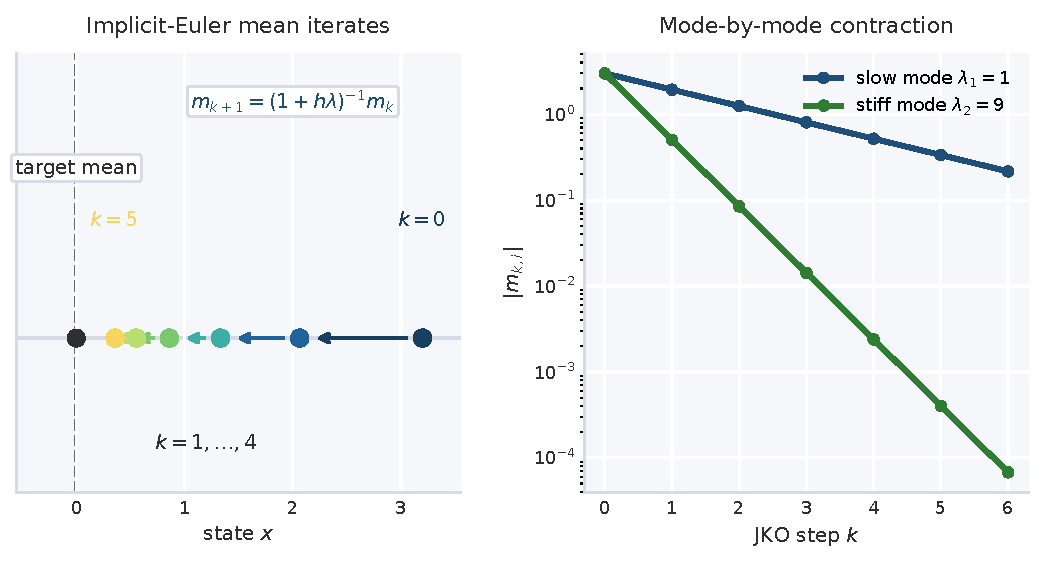
\includegraphics[width=0.9\linewidth]{figures/handouts/langevin_entropy_transport/fig_gaussian_jko_steps}
  \caption{For a quadratic target, restricting JKO to translated Gaussians keeps the covariance fixed and moves only the mean.
  That mean update is exactly implicit Euler, and in diagonal coordinates each mode contracts by $(1+h\lambda_i)^{-1}$, so stiff directions settle faster.}
  \label{fig:gaussian-jko}
\end{figure}

\Cref{fig:gaussian-jko} makes the same point visually.
The left panel shows the mean locations of those translated-Gaussian minimizers.
Because the covariance is fixed inside this restricted family, tracking the means is enough to see the entire update.
The right panel shows the mode-by-mode damping from \eqref{eq:jko-modewise}.

\begin{exercise}[Computing the Gaussian JKO mean step]
\label{ex:gaussian-jko-mean}
Work in the translated Gaussian family from \Cref{prop:gaussian-jko-mean}.
\begin{enumerate}[leftmargin=*]
  \item Show that $W_2^2(\rho_m,\rho_{m_k})=\norm{m-m_k}_2^2$.
  \item Show that $\mathcal{F}(\rho_m)-\mathcal{F}(\pi)=\tfrac12 m^\top Hm$.
  \item Derive \eqref{eq:gaussian-jko-mean} and the mode-by-mode contraction formula \eqref{eq:jko-modewise}.
\end{enumerate}
\end{exercise}
\SolutionBox[16]{%
\begin{enumerate}[leftmargin=*]
  \item Since $\rho_m$ and $\rho_{m_k}$ have the same covariance, the optimal transport is just translation by $m-m_k$, so
  \[
  W_2^2(\rho_m,\rho_{m_k})=\norm{m-m_k}_2^2.
  \]
  \item By \Cref{prop:free-energy-kl},
  \[
  \mathcal{F}(\rho_m)-\mathcal{F}(\pi)=D_{\mathrm{KL}}(\rho_m\|\pi).
  \]
  For Gaussians with equal covariance $H^{-1}$, the KL divergence reduces to the quadratic mean term
  \[
  D_{\mathrm{KL}}(\rho_m\|\pi)=\frac12 m^\top Hm.
  \]
  \item Therefore the JKO objective restricted to translated Gaussians is
  \[
  \Phi(m)=\frac{1}{2h}\norm{m-m_k}_2^2+\frac12 m^\top Hm.
  \]
  Its gradient is
  \[
  \nabla \Phi(m)=\frac{1}{h}(m-m_k)+Hm.
  \]
  Setting this to zero at the minimizer gives
  \[
  \frac{1}{h}(m_{k+1}-m_k)+Hm_{k+1}=0,
  \]
  hence
  \[
  m_{k+1}=(I_d+hH)^{-1}m_k.
  \]
  If $H=Q\Lambda Q^\top$ and $u_k=Q^\top m_k$, then
  \[
  u_{k+1}=Q^\top(I_d+hH)^{-1}Q\,u_k=(I_d+h\Lambda)^{-1}u_k,
  \]
  so each coordinate satisfies
  \[
  u_{k+1,i}=\frac{1}{1+h\lambda_i}u_{k,i}.
  \]
\end{enumerate}%
}

\subsection{The implicit velocity law}
\label{subsec:jko-velocity-law}

The mean calculation shows the basic mechanism in one tractable family, but the full measure-space update has an equally important first-order condition.
If $\rho_{k+1}$ is a smooth positive minimizer of \eqref{eq:jko-step} and $T_{k+1}$ is the optimal transport map from $\rho_{k+1}$ to $\rho_k$, then the Euler--Lagrange condition can be written as
\begin{equation}
  \frac{\operatorname{id}-T_{k+1}}{h}
  =
  -\nabla\bigl(U+\log \rho_{k+1}\bigr)
  \qquad \rho_{k+1}\text{-a.e.}
  \label{eq:jko-euler-lagrange}
\end{equation}
see \citet[\S4.5, Prop.~4.16]{santambrogio_2016_gradient_flows_overview}.
This is exactly the measure-space analogue of the implicit Euler equation
\[
\frac{x_{k+1}-x_k}{h}=-\nabla F(x_{k+1}).
\]
The transport displacement per unit time equals the free-energy velocity, evaluated at the \emph{new} density.

\subsection{The general JKO theorem}
\label{subsec:jko-general-theorem}

The full theorem is much deeper than the Gaussian example, and we do not try to reproduce the compactness proof here.
For our purposes, the conclusion is the key point.

\begin{theorem}[JKO scheme for Fokker--Planck, cited]
\label{thm:jko-general}
In the regular setting treated in \citet[\S4.5, Eq.~(4.13), Prop.~4.14, Prop.~4.19, pp.~37--42]{santambrogio_2016_gradient_flows_overview}, each minimization problem in \eqref{eq:jko-step} is well posed, and as $h\downarrow 0$ the recursive minimizers admit piecewise constant or geodesic interpolants that converge to the solution of the corresponding Fokker--Planck equation with the prescribed initial density.
In this sense, the Fokker--Planck equation is the $W_2$-gradient flow of free energy.
\end{theorem}

The cited proof is written on a compact domain with a $C^1$ confinement potential.
For the Langevin setting on $\R^d$, one imposes the corresponding confinement and integrability assumptions to recover the same minimizing-movement picture.
That theorem is the mathematical heart of the note.
It upgrades the formal continuity-equation picture from \Cref{prop:fokker-planck-continuity} into a precise variational statement: Langevin is not merely a diffusion with invariant law $\pi$; it is the steepest descent of $\mathcal{F}$ in Wasserstein geometry.
The right way to read the theorem is as an infinite-dimensional implicit-Euler convergence statement.
For each fixed $h$, the JKO rule produces a discrete descent path of densities.
As the step size shrinks, those variational steps converge to the actual Fokker--Planck evolution.
So the proximal picture is not just an analogy borrowed from optimization language; it is a literal construction of the PDE.

\section{An exact decay identity}
\label{sec:entropy-dissipation}

JKO identifies the geometry of the flow.
The next step is to compute an exact time derivative.
That is what turns the variational picture into a quantitative convergence argument.

\subsection{The instantaneous decay rate}
\label{subsec:fisher-dissipation}

The quantity that records this instantaneous decay rate is the \emph{relative Fisher information}.
It is defined by
\begin{equation}
  I(\rho\|\pi)
  :=
  \int_{\R^d}
  \norm{\nabla\log\frac{\rho}{\pi}}_2^2\,\rho\,dx.
  \label{eq:relative-fisher}
\end{equation}
Because $\log \pi=-U-\log Z$, this can also be written as
\[
I(\rho\|\pi)
=
\int \norm{\nabla(U+\log\rho)}_2^2\,\rho\,dx.
\]
It measures the squared size of the free-energy slope.

\begin{proposition}[Entropy dissipation identity]
\label{prop:entropy-dissipation}
Let $(\rho_t)_{t\ge 0}$ solve the Langevin Fokker--Planck equation.
Under the smoothness and decay assumptions needed for integration by parts,
\begin{equation}
  \frac{d}{dt}D_{\mathrm{KL}}(\rho_t\|\pi)
  =
  -I(\rho_t\|\pi).
  \label{eq:entropy-dissipation}
\end{equation}
\end{proposition}

\begin{proof}
Using mass conservation, $\int \partial_t \rho_t\,dx=0$, we may differentiate the entropy functional as
\begin{align*}
  \frac{d}{dt}D_{\mathrm{KL}}(\rho_t\|\pi)
  &=
  \int \log\frac{\rho_t}{\pi}\,\partial_t \rho_t\,dx.
\end{align*}
From \Cref{prop:fokker-planck-continuity},
\[
\partial_t \rho_t
=
\nabla\cdot\!\left(\rho_t\nabla\log\frac{\rho_t}{\pi}\right).
\]
Therefore
\begin{align*}
  \frac{d}{dt}D_{\mathrm{KL}}(\rho_t\|\pi)
  &=
  \int \log\frac{\rho_t}{\pi}
  \nabla\cdot\!\left(\rho_t\nabla\log\frac{\rho_t}{\pi}\right)\,dx \\
  &=
  -\int
  \norm{\nabla\log\frac{\rho_t}{\pi}}_2^2
  \rho_t\,dx \\
  &=
  -I(\rho_t\|\pi),
\end{align*}
which is \eqref{eq:entropy-dissipation}.%
\end{proof}

\Cref{prop:entropy-dissipation} is the exact dynamic counterpart of \Cref{prop:free-energy-kl}.
Relative entropy is the gap to equilibrium, and Fisher information is the instantaneous rate at which Langevin closes that gap.

\begin{exercise}[Deriving entropy dissipation]
\label{ex:entropy-dissipation}
Starting from \Cref{eq:fokker-planck-continuity}, prove \Cref{eq:entropy-dissipation}.
Then explain why $I(\rho_t\|\pi)=0$ forces $\rho_t=\pi$ under mild connectedness assumptions.
\end{exercise}
\SolutionBox[14]{%
We begin with
\[
D_{\mathrm{KL}}(\rho_t\|\pi)=\int \rho_t \log\frac{\rho_t}{\pi}\,dx.
\]
Since $\int \partial_t \rho_t\,dx=0$,
\[
\frac{d}{dt}D_{\mathrm{KL}}(\rho_t\|\pi)
=
\int \log\frac{\rho_t}{\pi}\,\partial_t \rho_t\,dx.
\]
Using the continuity-equation form,
\[
\partial_t \rho_t
=
\nabla\cdot\!\left(\rho_t\nabla\log\frac{\rho_t}{\pi}\right),
\]
we obtain
\begin{align*}
\frac{d}{dt}D_{\mathrm{KL}}(\rho_t\|\pi)
&=
\int \log\frac{\rho_t}{\pi}\,
\nabla\cdot\!\left(\rho_t\nabla\log\frac{\rho_t}{\pi}\right)\,dx \\
&=
-\int \norm{\nabla\log\frac{\rho_t}{\pi}}_2^2\,\rho_t\,dx \\
&=
-I(\rho_t\|\pi).
\end{align*}
If $I(\rho_t\|\pi)=0$, then $\nabla\log(\rho_t/\pi)=0$ almost everywhere on the support of $\rho_t$, so $\rho_t/\pi$ is constant on each connected component.
Both densities integrate to $1$, so that constant must be $1$, hence $\rho_t=\pi$ almost everywhere.%
}

\subsection{An exact Ornstein--Uhlenbeck example}
\label{subsec:ou-example}

The entropy dissipation identity is completely explicit for Gaussian targets.
Let
\[
U(x)=\frac12 x^\top Hx,
\qquad
H\succ 0,
\qquad
\pi=\mathcal{N}(0,H^{-1}).
\]
Suppose the initial law is
\[
\rho_0=\mathcal{N}(m_0,H^{-1}),
\]
so the covariance already matches equilibrium.
Then the Langevin diffusion preserves Gaussianity and only the mean moves:
\[
\rho_t=\mathcal{N}(m_t,H^{-1}),
\qquad
m_t=e^{-Ht}m_0.
\]
Writing $m_{0,i}$ in an eigenbasis of $H$ with eigenvalues $\lambda_i$ gives
\begin{equation}
  D_{\mathrm{KL}}(\rho_t\|\pi)
  =
  \frac12\sum_{i=1}^d \lambda_i m_{0,i}^2 e^{-2\lambda_i t},
  \qquad
  I(\rho_t\|\pi)
  =
  \sum_{i=1}^d \lambda_i^2 m_{0,i}^2 e^{-2\lambda_i t}.
  \label{eq:ou-kl-fisher}
\end{equation}
Differentiating the first display immediately yields
\[
\frac{d}{dt}D_{\mathrm{KL}}(\rho_t\|\pi)
=
-I(\rho_t\|\pi).
\]
This example is worth keeping in mind because every later result here collapses to an exact mode-by-mode statement in this quadratic setting.

\section{When decay becomes a uniform rate}
\label{sec:lsi}

Entropy dissipation by itself is only an identity.
It tells us the instantaneous decay rate,
\[
\frac{d}{dt}D_{\mathrm{KL}}(\rho_t\|\pi)=-I(\rho_t\|\pi),
\]
but not whether that rate is uniformly large when the chain is still far from equilibrium.
In principle the Fisher information could be small even while the entropy gap is still substantial.
To turn dissipation into a quantitative rate, we need an inequality that forces a large entropy gap to come with a large slope.
The standard tool is the log-Sobolev inequality, and the Bakry--\'Emery criterion is the curvature condition that often guarantees it.

\subsection{A functional inequality that closes the estimate}
\label{subsec:lsi-decay}

A log-Sobolev inequality compares the entropy gap directly to its dissipation.
Because
\[
I(\rho\|\pi)=\int \norm{\nabla \log(\rho/\pi)(x)}_2^2\,\rho(x)\,dx,
\]
the Fisher information is the squared $L^2(\rho)$ size of the relative log-density gradient.
Geometrically, it measures how sharply the density ratio $\rho/\pi$ is still tilted across space.
The log-Sobolev inequality says that a distribution cannot keep a large free-energy gap while that relative tilt is uniformly tiny.
Equivalently, a large mismatch from equilibrium must leave enough slope for Langevin to keep pushing downhill.

\begin{definition}[Log-Sobolev inequality]
\label{def:lsi}
We say that $\pi$ satisfies a log-Sobolev inequality with constant $\alpha>0$ if
\begin{equation}
  D_{\mathrm{KL}}(\rho\|\pi)
  \le
  \frac{1}{2\alpha}I(\rho\|\pi)
  \qquad
  \text{for every smooth density }\rho.
  \label{eq:lsi}
\end{equation}
\end{definition}

\begin{proposition}[LSI implies exponential KL decay]
\label{prop:lsi-kl-decay}
If $\pi$ satisfies \eqref{eq:lsi} with constant $\alpha>0$, then every sufficiently regular Langevin solution satisfies
\begin{equation}
  D_{\mathrm{KL}}(\rho_t\|\pi)
  \le
  e^{-2\alpha t}D_{\mathrm{KL}}(\rho_0\|\pi).
  \label{eq:kl-exponential-decay}
\end{equation}
\end{proposition}

\begin{proof}
By \Cref{prop:entropy-dissipation},
\[
\frac{d}{dt}D_{\mathrm{KL}}(\rho_t\|\pi)
=
-I(\rho_t\|\pi).
\]
Applying the log-Sobolev inequality at time $t$ gives
\[
I(\rho_t\|\pi)\ge 2\alpha D_{\mathrm{KL}}(\rho_t\|\pi),
\]
hence
\[
\frac{d}{dt}D_{\mathrm{KL}}(\rho_t\|\pi)
\le
-2\alpha D_{\mathrm{KL}}(\rho_t\|\pi).
\]
Gronwall's inequality yields \eqref{eq:kl-exponential-decay}.%
\end{proof}

This is the precise place where ``strong log-concavity implies quantitative mixing'' becomes a theorem.
Once Fisher information dominates entropy, the free-energy gap decays exponentially.
The geometric message is that under an LSI the target has no extended almost-flat directions in which a nonequilibrium density can hide.
If $\rho_t$ still differs substantially from $\pi$, then the relative log-density must still have noticeable slope, so the Fokker--Planck flow cannot stall prematurely.

\subsection{The Gaussian benchmark}
\label{subsec:gaussian-lsi}

For the Gaussian target
\[
\gamma_m(dx)\propto e^{-\frac{m}{2}\norm{x}_2^2}\,dx,
\]
the correct LSI constant is $\alpha=m$.
One way to see that is to invoke the curvature criterion in the next subsection, since $\Hess U=mI_d$.
Inside the translated Gaussian family, the constant is visible exactly:
if $\rho=\mathcal{N}(a,m^{-1}I_d)$, then
\[
D_{\mathrm{KL}}(\rho\|\gamma_m)=\frac{m}{2}\norm{a}_2^2,
\qquad
I(\rho\|\gamma_m)=m^2\norm{a}_2^2,
\]
so equality holds in \eqref{eq:lsi}.
That is a useful sanity check.
The Gaussian measure is not merely an example where LSI is true; it is the model case where the constants are exact.

\subsection{Curvature gives LSI}
\label{subsec:bakry-emery}

The next question is where a bound like \eqref{eq:lsi} comes from.
For strongly log-concave targets, the answer is curvature.
If $U$ bends upward everywhere by at least a fixed quadratic amount, then the measure has no broad flat directions in which entropy can stay large while the free-energy slope becomes tiny.
The Bakry--\'Emery criterion turns that idea into a global log-Sobolev constant.

\begin{theorem}[Bakry--\'Emery criterion, cited]
\label{thm:bakry-emery}
Let $\pi(dx)=Z^{-1}e^{-U(x)}\,dx$ on $\R^d$, where $U\in C^2(\R^d)$ and $Z<\infty$.
If
\begin{equation}
  \Hess U(x)\succeq mI_d
  \qquad\text{for every }x\in\R^d
  \label{eq:bakry-emery-curvature}
\end{equation}
for some $m>0$, then $\pi$ satisfies a log-Sobolev inequality with constant $\alpha=m$.
\end{theorem}

We cite \citet[Thm.~2]{otto_villani_2000_talagrand_lsi} for this form of the theorem.
Historically it is the Bakry--\'Emery curvature condition.
The proof uses $\Gamma_2$-calculus rather than the transport arguments used in the surrounding development, so we do not reproduce it.

The geometric meaning of \eqref{eq:bakry-emery-curvature} is that the ambient space always looks at least as confining as a quadratic well.
If $U$ has a uniform quadratic lower bound on curvature, then the target has no flat directions that allow entropy to linger and no broad corridors in which mass can drift with only a weak restoring force.
Misplaced mass must create a visible change in the relative log-density, so the free-energy slope cannot be tiny unless the entropy gap is already small.
That is exactly what \eqref{eq:lsi} formalizes.
What makes the theorem powerful is that it is global.
The lower Hessian bound is required at every point, not just near the mode, and the conclusion controls every smooth density $\rho$.
One can think of $m$ as a universal restoring-force constant: no matter where mass moves, the landscape is always at least as curved as a quadratic well of curvature $m$.
Bakry--\'Emery says that this geometric fact is enough to force a uniform entropy-dissipation estimate.

\section{From entropy to transport}
\label{sec:entropy-to-transport}

We now have an exponential decay theorem in KL divergence.
For proving convergence, that is already enough.
The reason to keep going is that KL and Wasserstein distance answer different questions.
The KL divergence measures excess free energy, while $W_2$ measures how far the mass of $\rho_t$ still has to move in space to match $\pi$.
That geometric viewpoint is closer to the coupling language of the Sampling unit and the conditioning language of the Optimization unit, so it is worth translating entropy control into transport control as well.

\begin{definition}[Talagrand's $T_2$ inequality]
\label{def:t2}
We say that $\pi$ satisfies $T_2(\alpha)$ if
\begin{equation}
  W_2^2(\rho,\pi)
  \le
  \frac{2}{\alpha}D_{\mathrm{KL}}(\rho\|\pi)
  \qquad
  \text{for every density }\rho.
  \label{eq:t2}
\end{equation}
\end{definition}

\begin{theorem}[Otto--Villani, cited]
\label{thm:otto-villani}
Let $\pi(dx)=Z^{-1}e^{-U(x)}\,dx$ be a probability measure on $\R^d$ with finite second moment, where $U\in C^2(\R^d)$ and
\[
\Hess U(x)\succeq C I_d
\qquad\text{for every }x\in\R^d
\]
for some $C\in\R$.
If $\pi$ satisfies a log-Sobolev inequality with constant $\alpha>0$, then $\pi$ also satisfies $T_2(\alpha)$.
\end{theorem}

This is \citet[Thm.~1]{otto_villani_2000_talagrand_lsi}.
It says that once entropy is controlled, the amount of spatial transport still needed to reach equilibrium is controlled automatically.
That is not obvious a priori because the two quantities measure different kinds of mismatch.
The KL divergence compares density values pointwise, while $W_2$ measures the cost of rearranging mass in space.
The theorem says that an LSI is strong enough to connect them: under sufficient curvature, any large remaining transport cost would itself force a large entropy gap.
So transport control is not an extra ingredient added on top of entropy control; it is a geometric consequence of the same inequality.

\begin{samepage}
\begin{corollary}[Wasserstein decay from LSI]
\label{cor:wasserstein-decay}
Under the hypotheses of \Cref{thm:otto-villani}, every sufficiently regular Langevin solution satisfies
\begin{equation}
  W_2(\rho_t,\pi)
  \le
  \sqrt{\frac{2}{\alpha}}\,
  e^{-\alpha t}
  \sqrt{D_{\mathrm{KL}}(\rho_0\|\pi)}.
  \label{eq:w2-decay}
\end{equation}
\end{corollary}
\end{samepage}

\begin{proof}
Combine \Cref{thm:otto-villani} with \Cref{prop:lsi-kl-decay}:
\[
W_2^2(\rho_t,\pi)
\le
\frac{2}{\alpha}D_{\mathrm{KL}}(\rho_t\|\pi)
\le
\frac{2}{\alpha}e^{-2\alpha t}D_{\mathrm{KL}}(\rho_0\|\pi).
\]
Taking square roots gives \eqref{eq:w2-decay}.%
\end{proof}

For the Gaussian family from \Cref{subsec:gaussian-lsi}, the bridge is exact on translated states:
if $\rho=\mathcal{N}(a,m^{-1}I_d)$ and $\gamma_m=\mathcal{N}(0,m^{-1}I_d)$, then
\[
W_2^2(\rho,\gamma_m)=\norm{a}_2^2=\frac{2}{m}D_{\mathrm{KL}}(\rho\|\gamma_m).
\]
So the LSI-to-$T_2$ story is not merely qualitative.
Its constants are already sharp in the Gaussian model.

\begin{exercise}[From LSI to a Wasserstein bound]
\label{ex:lsi-to-w2}
Assume $\pi$ satisfies LSI$(\alpha)$.
\begin{enumerate}[leftmargin=*]
  \item Use \Cref{prop:entropy-dissipation} to derive \Cref{eq:kl-exponential-decay}.
  \item Combine that with \Cref{eq:t2} to prove \Cref{eq:w2-decay}.
  \item Verify directly in the translated Gaussian family that $T_2(\alpha)$ holds with equality.
\end{enumerate}
\end{exercise}
\SolutionBox[14]{%
\begin{enumerate}[leftmargin=*]
  \item By entropy dissipation,
  \[
  \frac{d}{dt}D_{\mathrm{KL}}(\rho_t\|\pi)=-I(\rho_t\|\pi).
  \]
  The LSI bound gives
  \[
  I(\rho_t\|\pi)\ge 2\alpha D_{\mathrm{KL}}(\rho_t\|\pi),
  \]
  so
  \[
  \frac{d}{dt}D_{\mathrm{KL}}(\rho_t\|\pi)\le -2\alpha D_{\mathrm{KL}}(\rho_t\|\pi).
  \]
  Gronwall yields
  \[
  D_{\mathrm{KL}}(\rho_t\|\pi)\le e^{-2\alpha t}D_{\mathrm{KL}}(\rho_0\|\pi).
  \]
  \item Talagrand's inequality gives
  \[
  W_2^2(\rho_t,\pi)\le \frac{2}{\alpha}D_{\mathrm{KL}}(\rho_t\|\pi).
  \]
  Substituting the KL decay bound,
  \[
  W_2^2(\rho_t,\pi)\le \frac{2}{\alpha}e^{-2\alpha t}D_{\mathrm{KL}}(\rho_0\|\pi),
  \]
  and taking square roots gives \eqref{eq:w2-decay}.
  \item For $\gamma_\alpha=\mathcal{N}(0,\alpha^{-1}I_d)$ and $\rho=\mathcal{N}(a,\alpha^{-1}I_d)$,
  \[
  W_2^2(\rho,\gamma_\alpha)=\norm{a}_2^2
  \]
  because the optimal transport is translation by $a$, while
  \[
  D_{\mathrm{KL}}(\rho\|\gamma_\alpha)=\frac{\alpha}{2}\norm{a}_2^2.
  \]
  Hence
  \[
  W_2^2(\rho,\gamma_\alpha)=\frac{2}{\alpha}D_{\mathrm{KL}}(\rho\|\gamma_\alpha),
  \]
  so $T_2(\alpha)$ is attained exactly on this translated Gaussian family.%
\end{enumerate}
}

\section{Preconditioning and a real posterior}
\label{sec:preconditioning-real-data}

The functional-inequality chain explains why Langevin converges.
The final question is where the constants come from in practice.
For quadratic or locally quadratic targets, the answer is geometric: the relevant rates are the eigenvalues of the preconditioned Hessian.

\subsection{Quadratic targets and the rate matrix}
\label{subsec:preconditioning-quadratic}

Now return to geometry.
Consider the preconditioned overdamped Langevin diffusion
\begin{equation}
  dX_t=-M\nabla U(X_t)\,dt+\sqrt{2M}\,dB_t,
  \label{eq:preconditioned-langevin}
\end{equation}
where $M\succ 0$ is a fixed symmetric positive-definite matrix.
For a quadratic potential centered at $x_\star$,
\[
U(x)=\frac12 (x-x_\star)^\top H(x-x_\star),
\qquad
H\succ 0,
\]
the geometry is again exact.

\begin{proposition}[The relevant rate matrix is $M^{1/2}HM^{1/2}$]
\label{prop:preconditioned-rate-matrix}
Let $Y_t:=M^{-1/2}(X_t-x_\star)$.
Then \eqref{eq:preconditioned-langevin} becomes
\begin{equation}
  dY_t=-A Y_t\,dt+\sqrt{2}\,dB_t,
  \qquad
  A:=M^{1/2}HM^{1/2}.
  \label{eq:preconditioned-ou}
\end{equation}
Hence the mode-by-mode decay rates are the eigenvalues of $A$, not of $H$ alone.
In particular, if $M=H^{-1}$, then $A=I_d$ and all local modes are equalized.
\end{proposition}

\begin{proof}
Write $X_t=x_\star+M^{1/2}Y_t$.
Then
\[
dX_t=M^{1/2}dY_t,
\qquad
\nabla U(X_t)=H(X_t-x_\star)=HM^{1/2}Y_t.
\]
Substituting into \eqref{eq:preconditioned-langevin},
\[
M^{1/2}dY_t=-MHM^{1/2}Y_t\,dt+\sqrt{2M}\,dB_t.
\]
Multiplying by $M^{-1/2}$ gives
\[
dY_t=-M^{1/2}HM^{1/2}Y_t\,dt+\sqrt{2}\,dB_t,
\]
which is \eqref{eq:preconditioned-ou}.%
\end{proof}

The local conclusion is immediate.
Whitening is not mysterious.
It is exactly the choice of $M$ that turns the local quadratic surrogate into an isotropic Ornstein--Uhlenbeck process.

The entropy and transport quantities from earlier sections are also explicit here.
If the transformed process starts from
\[
Y_0\sim \mathcal{N}(m_0,A^{-1}),
\]
then
\[
Y_t\sim \mathcal{N}(e^{-At}m_0,A^{-1}),
\]
so in an eigenbasis of $A$ with eigenvalues $\nu_i$ and coordinates $c_i$ of $m_0$,
\begin{equation}
  D_{\mathrm{KL}}(\rho_t\|\pi)
  =
  \frac12\sum_i \nu_i c_i^2 e^{-2\nu_i t},
  \qquad
  I(\rho_t\|\pi)
  =
  \sum_i \nu_i^2 c_i^2 e^{-2\nu_i t},
  \qquad
  W_2^2(\rho_t,\pi)
  =
  \sum_i c_i^2 e^{-2\nu_i t}.
  \label{eq:preconditioned-decay-formulas}
\end{equation}
When $M=H^{-1}$, all $\nu_i$ become $1$, so every mode decays on the same time scale.

\begin{figure}[t]
  \centering
  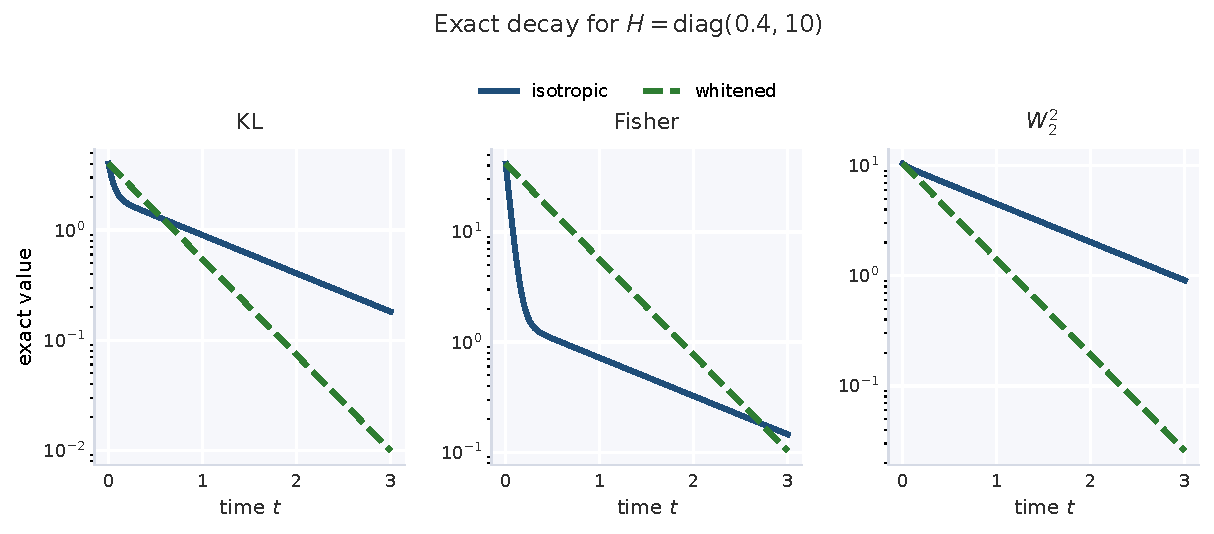
\includegraphics[width=0.95\linewidth]{figures/handouts/langevin_entropy_transport/fig_gaussian_decay_preconditioning}
  \caption{For an anisotropic Gaussian target, KL, Fisher information, and $W_2^2$ decay exactly under the local Ornstein--Uhlenbeck dynamics.
  Whitening turns the rate matrix into the identity and removes the slow mode.}
  \label{fig:gaussian-preconditioning}
\end{figure}

\Cref{fig:gaussian-preconditioning} shows \eqref{eq:preconditioned-decay-formulas} for a simple two-dimensional quadratic target.
The visual simplification reflects an analytic one.
Whitening changes the exact exponents appearing in every convergence quantity derived above.

\subsection{Bayesian logistic regression on the Problem Set 2 data}
\label{subsec:logistic-real-data}

To keep the real-data example aligned with the notes, we return to the regularized logistic-regression model that runs through the Optimization unit and reappears in Problem Set~2.
The dataset has five predictors and a binary response.
In the optimization material, this model supplied explicit gradients, Hessians, and the MAP/Laplace calculation.
Here the same local quadratic surrogate serves a different purpose: it reveals the local rate matrix seen by overdamped Langevin near the MAP.

Write
\[
\beta=(\beta_0,\beta_1,\dots,\beta_5)^\top,
\qquad
\tilde x_i=(1,x_{i1},\dots,x_{i5})^\top.
\]
We also keep the same isotropic Gaussian prior as in Problem Set~2,
\[
\beta\sim \mathcal{N}(0,100 I_6),
\]
so the prior precision is $\lambda=0.01$.
The negative log posterior is
\begin{equation}
  U(\beta)
  =
  \sum_{i=1}^n \Bigl[\log\!\bigl(1+e^{\tilde x_i^\top\beta}\bigr)-y_i \tilde x_i^\top\beta\Bigr]
  +
  \frac{\lambda}{2}\norm{\beta}_2^2.
  \label{eq:logistic-posterior}
\end{equation}
If $p_i(\beta)=\sigma(\tilde x_i^\top\beta)$ with $\sigma(t)=1/(1+e^{-t})$, then
\[
\nabla U(\beta)=X^\top(p(\beta)-y)+\lambda\beta,
\qquad
\Hess U(\beta)=X^\top W(\beta)X+\lambda I_6,
\]
where $W(\beta)$ is diagonal with entries $p_i(\beta)(1-p_i(\beta))$.

We compute the MAP estimate $\beta_{\mathrm{MAP}}$ numerically and use the Hessian
\[
H_{\mathrm{MAP}}:=\Hess U(\beta_{\mathrm{MAP}})
\]
as a local Gaussian surrogate.
This is exactly the Laplace approximation, and we use it only locally.
The claim is not that the posterior is globally Gaussian.
The claim is that the Hessian near the MAP reveals which local preconditioner equalizes the quadratic surrogate.

\begin{figure}[t]
  \centering
  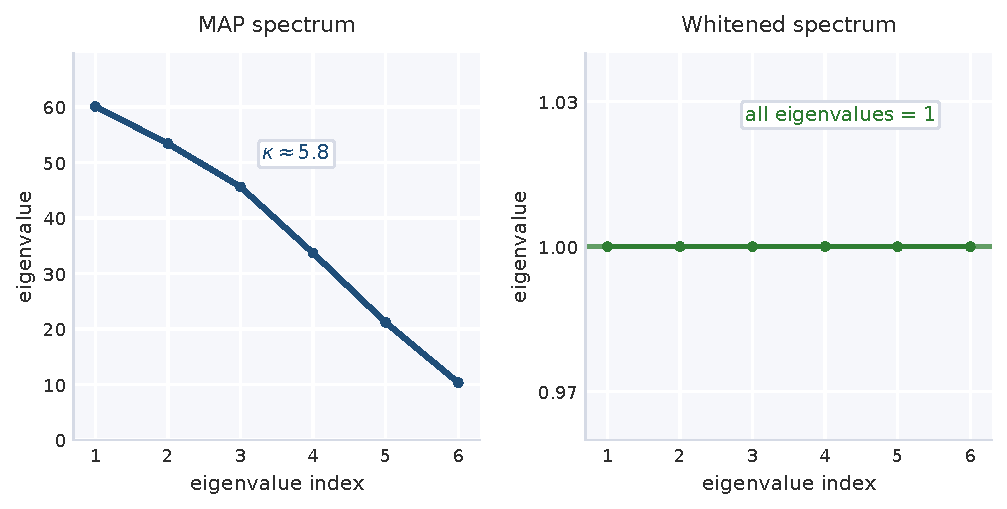
\includegraphics[width=0.92\linewidth]{figures/handouts/langevin_entropy_transport/fig_logistic_hessian_spectrum}
  \caption{The Problem Set 2 Bayesian logistic posterior has a nontrivial MAP Hessian spectrum.
  Whitening with $H_{\mathrm{MAP}}^{-1/2}$ collapses the local spectrum to $1$.}
  \label{fig:logistic-spectrum}
\end{figure}

\Cref{fig:logistic-spectrum} shows the full Hessian spectrum.
The raw local condition number is about $5.8$.
That is not extreme, but it is large enough to make the soft/stiff splitting visible in a familiar course example.
That spectrum is the continuous-time Langevin analogue of the conditioning language from the Optimization unit and the Sampling unit's gradient-based MCMC subsection.

\begin{figure}[t]
  \centering
  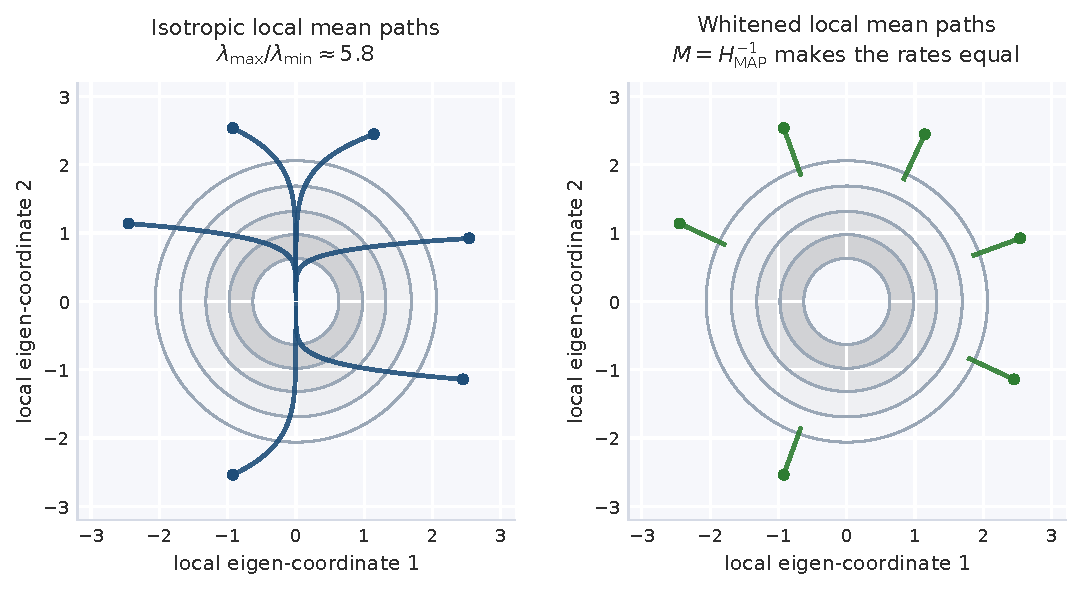
\includegraphics[width=0.92\linewidth]{figures/handouts/langevin_entropy_transport/fig_logistic_laplace_trajectories}
  \caption{The softest/stiffest eigenspace of the Laplace surrogate around the MAP.
  Without preconditioning, local mean paths pinch first along the stiff direction and only later move along the soft direction; local whitening equalizes the contraction rates.}
  \label{fig:logistic-trajectories}
\end{figure}

\Cref{fig:logistic-trajectories} turns the spectrum into a local picture.
Because this model has only six parameters, the figure uses the softest and stiffest eigendirections directly.
The message is the same in either case.
Without preconditioning, the local mean paths collapse first in the stiff direction while progress in the soft direction lags behind.
With $M=H_{\mathrm{MAP}}^{-1}$, the local quadratic surrogate has balanced rates.

This is the right closing connection to the course's conditioning language.
For overdamped Langevin, preconditioning changes the exact rate matrix controlling entropy dissipation and transport contraction.
The same local Hessian picture is what later makes mass-matrix choices matter in the Augmented-state sampling unit's HMC/NUTS development.

\begin{exercise}[Reading the local Hessian geometry]
\label{ex:logistic-preconditioner}
Use \Cref{prop:preconditioned-rate-matrix}, \Cref{fig:logistic-spectrum}, and \Cref{fig:logistic-trajectories}.
\begin{enumerate}[leftmargin=*]
  \item Explain why a spread in the eigenvalues of $H_{\mathrm{MAP}}$ produces multiple local mixing time scales for isotropic Langevin.
  \item Show that choosing $M=H_{\mathrm{MAP}}^{-1}$ makes the local rate matrix equal to the identity.
  \item Why is $H_{\mathrm{MAP}}^{-1}$ the natural quadratic preconditioner, up to an overall scalar factor?
\end{enumerate}
\end{exercise}
\SolutionBox[14]{%
\begin{enumerate}[leftmargin=*]
  \item In the quadratic surrogate, isotropic Langevin corresponds to $M=I_d$, so the local rate matrix is just $H_{\mathrm{MAP}}$.
  Its eigenvalues are the mode-by-mode contraction rates.
  If those eigenvalues vary widely, some directions equilibrate quickly while others remain slow, creating multiple local time scales.
  \item By \Cref{prop:preconditioned-rate-matrix},
  \[
  A=M^{1/2}H_{\mathrm{MAP}}M^{1/2}.
  \]
  Setting $M=H_{\mathrm{MAP}}^{-1}$ gives
  \[
  A=H_{\mathrm{MAP}}^{-1/2}H_{\mathrm{MAP}}H_{\mathrm{MAP}}^{-1/2}=I_d.
  \]
  So all local contraction rates become $1$.
  \item If the goal is to equalize the quadratic modes, then we want $A$ to be proportional to the identity.
  That means
  \[
  M^{1/2}H_{\mathrm{MAP}}M^{1/2}=cI_d
  \]
  for some scalar $c>0$, which is equivalent to
  \[
  M=c\,H_{\mathrm{MAP}}^{-1}.
  \]
  Thus $H_{\mathrm{MAP}}^{-1}$ is the natural local quadratic preconditioner, with any extra scalar factor only changing the overall time scale.%
\end{enumerate}
}

There is also a discrete-time algorithmic payoff.
Once one has an LSI and enough smoothness, these continuous-time decay arguments feed directly into nonasymptotic ULA theory; see \citet[\S3.1, Thm.~1]{vempala_wibisono_2019_ula_isoperimetry}.
The point of that cited result is not that Euler discretization exactly preserves the diffusion analysis.
Rather, good continuous-time geometry survives discretization up to a controlled error, so the same inequalities lead to quantitative bounds for an actual algorithm.
The course-level synthesis is now clear.
Free energy is the Lyapunov functional, JKO is the proximal structure, Fisher information supplies dissipation, LSI turns dissipation into a uniform rate, Talagrand converts that rate into transport control, and preconditioning changes the constants by changing the local geometry.
Carried back to the main notes, this is the optimization story returning in measure space: descent becomes entropy dissipation, proximal structure becomes JKO, and conditioning still determines which directions are easy and which are slow.

\bibliographystyle{plainnat}
\makeatletter
\begingroup
\let\input@path\@empty
\IfFileExists{references.bib}{%
  \gdef\stat221bibpath{references}%
}{%
  \IfFileExists{../references.bib}{%
    \gdef\stat221bibpath{../references}%
  }{%
    \gdef\stat221bibpath{../../references}%
  }%
}
\endgroup
\makeatother
\bibliography{\stat221bibpath}

\end{document}
"
%   (Low-level direct build: if you invoke latexmk manually, set -jobname to the
%    titled output so the compiled PDF matches the standard naming scheme.)
\newif\ifshowsolutions
\showsolutionsfalse
\ifdefined\STATshowsolutions
  \showsolutionstrue
\fi
\ifcsname STAT221SOLUTIONS\endcsname
  \showsolutionstrue
\fi

% Solutions/workspace boxes (controlled by \ifshowsolutions).
% Usage: \SolutionBox[<workspace lines>]{<solution body>}
\newcommand{\SolutionBox}[2][10]{%
  \ifshowsolutions
    \begin{tcolorbox}[stat221panelgray,title={Solution}]
    #2
    \end{tcolorbox}
  \else
    \begin{tcolorbox}[stat221panelgray,unbreakable,title={Workspace}]
    \vspace{#1\baselineskip}
    \end{tcolorbox}
  \fi
}

\title{How do entropy and transport control Langevin convergence?}
\author{}
\date{}

\begin{document}
\maketitle

\section[Entropy, transport, and Langevin]{How do entropy and transport control Langevin convergence?}
\label{sec:langevin-handout-opening}

This handout takes one question from the Sampling unit and studies it in continuous time: how fast does the overdamped Langevin law approach equilibrium, and which geometric assumptions control that rate?
The diffusion itself is
\[
dX_t=-\nabla U(X_t)\,dt+\sqrt{2}\,dB_t,
\]
with stationary law
\[
\pi(x)=Z^{-1}e^{-U(x)}.
\]
Here $Z=\int_{\R^d} e^{-U(x)}\,dx$ is assumed finite, and the evolving object is the law $\rho_t=\mathcal{L}(X_t)$ when $X_0$ does not start from equilibrium.
The main quantities will be the free-energy gap, its dissipation along the Langevin flow, and the transport inequalities that turn dissipation into quantitative convergence.

This viewpoint extends the Sampling unit's gradient-based MCMC subsection, reuses the Optimization unit's language of objectives, proximal structure, and conditioning in measure space, and feeds directly into the Augmented-state sampling unit.
There the same local geometry drives HMC and NUTS through momentum-carrying trajectories rather than one-step Langevin corrections.

There is also a concrete geometric reason to care.
For a quadratic target
\[
U(x)=\frac12 x^\top Hx,
\]
every mode in an eigenbasis of $H$ relaxes at its own exponential rate.
If $H$ is poorly conditioned, then one slow direction controls the last stage of convergence even when the other directions have already equilibrated.
So even in the friendliest Gaussian case, convergence is already controlled by geometry.
The rest of the note develops the general version of that picture:
we identify a free-energy gap to equilibrium, compute its dissipation along the Langevin flow, convert that dissipation into explicit entropy and transport rates, and then read off how preconditioning changes the governing matrix in quadratic and locally quadratic models.

Throughout we work in the smooth, rapidly decaying setting when we differentiate under the integral sign or integrate by parts.
Those formal calculations are the right ones, and the cited theorems extend them to broader classes of densities.

\section{A notion of distance to equilibrium}
\label{sec:free-energy-fokker-planck}

The first task is to identify the right notion of distance to equilibrium.
For Langevin, the natural candidate is not Euclidean distance between points but a functional on densities.
The standard object here is the free-energy gap, and the corresponding density evolution is governed by the Fokker--Planck equation.

\subsection{Relative entropy is a free-energy gap}
\label{subsec:free-energy-gap}

Fix a potential $U:\R^d\to\R$ and define the target density
\[
\pi(x)=Z^{-1}e^{-U(x)},
\qquad
Z=\int_{\R^d} e^{-U(x)}\,dx.
\]
For a probability density $\rho$ we define the free energy
\begin{equation}
  \mathcal{F}(\rho)
  :=
  \int_{\R^d} U(x)\rho(x)\,dx
  +
  \int_{\R^d} \rho(x)\log \rho(x)\,dx.
  \label{eq:free-energy-definition}
\end{equation}
The first term is potential energy.
The second is minus the Shannon entropy, so $\mathcal{F}$ is the natural energy--entropy tradeoff for Langevin diffusion.

\begin{proposition}[Relative entropy equals the free-energy gap]
\label{prop:free-energy-kl}
For every probability density $\rho$ with finite free energy,
\begin{equation}
  D_{\mathrm{KL}}(\rho\|\pi)
  =
  \mathcal{F}(\rho)-\mathcal{F}(\pi).
  \label{eq:free-energy-gap}
\end{equation}
In particular,
\[
\mathcal{F}(\pi)=-\log Z,
\]
so minimizing free energy is the same as minimizing relative entropy to $\pi$.
\end{proposition}

\begin{proof}
Since $\log \pi(x)=-U(x)-\log Z$,
\begin{align*}
  D_{\mathrm{KL}}(\rho\|\pi)
  &=
  \int \rho(x)\log\frac{\rho(x)}{\pi(x)}\,dx \\
  &=
  \int \rho(x)\log \rho(x)\,dx
  +
  \int U(x)\rho(x)\,dx
  +
  \log Z \\
  &=
  \mathcal{F}(\rho)+\log Z.
\end{align*}
Applying the same identity with $\rho=\pi$ gives
\[
0=D_{\mathrm{KL}}(\pi\|\pi)=\mathcal{F}(\pi)+\log Z,
\]
so $\mathcal{F}(\pi)=-\log Z$.
Substituting this into the first formula yields \eqref{eq:free-energy-gap}.%
\end{proof}

\Cref{prop:free-energy-kl} is the basic dictionary for the rest of the note.
The object that decreases along Langevin is not an ad hoc Lyapunov function.
It is exactly the distance to equilibrium measured in relative entropy.

\begin{exercise}[Deriving the free-energy identity]
\label{ex:free-energy-gap}
Starting from \Cref{eq:free-energy-definition} and $\pi(x)=Z^{-1}e^{-U(x)}$, derive \Cref{eq:free-energy-gap}.
Then show directly that $\pi$ minimizes $\mathcal{F}$ over all densities.
\end{exercise}
\SolutionBox[12]{%
We expand the logarithm of the target:
\[
\log \pi(x)=-U(x)-\log Z.
\]
Therefore
\begin{align*}
  D_{\mathrm{KL}}(\rho\|\pi)
  &=
  \int \rho(x)\log\frac{\rho(x)}{\pi(x)}\,dx \\
  &=
  \int \rho(x)\log \rho(x)\,dx
  +
  \int U(x)\rho(x)\,dx
  +
  \log Z \\
  &=
  \mathcal{F}(\rho)+\log Z.
\end{align*}
Setting $\rho=\pi$ gives
\[
0=D_{\mathrm{KL}}(\pi\|\pi)=\mathcal{F}(\pi)+\log Z,
\]
so $\mathcal{F}(\pi)=-\log Z$, hence
\[
D_{\mathrm{KL}}(\rho\|\pi)=\mathcal{F}(\rho)-\mathcal{F}(\pi).
\]
Because relative entropy is always nonnegative and vanishes only when $\rho=\pi$ almost everywhere, $\pi$ is the unique minimizer of $\mathcal{F}$.%
}

\subsection{Langevin as a continuity equation}
\label{subsec:fokker-planck-continuity}

The overdamped Langevin diffusion is
\begin{equation}
  dX_t=-\nabla U(X_t)\,dt+\sqrt{2}\,dB_t.
  \label{eq:overdamped-langevin}
\end{equation}
If $\rho_t$ denotes the density of $X_t$, then $\rho_t$ solves the Fokker--Planck equation
\begin{equation}
  \partial_t \rho_t
  =
  \nabla\cdot(\rho_t\nabla U)+\Delta \rho_t.
  \label{eq:fokker-planck-basic}
\end{equation}
The key rewrite is that the diffusion term can be absorbed into the logarithmic derivative of $\rho_t$.

\begin{proposition}[Continuity-equation form of Fokker--Planck]
\label{prop:fokker-planck-continuity}
Assume $\rho_t$ is smooth and strictly positive.
Then \eqref{eq:fokker-planck-basic} can be written as
\begin{equation}
  \partial_t \rho_t
  =
  \nabla\cdot\!\bigl(\rho_t \nabla(U+\log\rho_t)\bigr)
  =
  -\nabla\cdot(\rho_t v_t),
  \label{eq:fokker-planck-continuity}
\end{equation}
with velocity field
\begin{equation}
  v_t
  =
  -\nabla\bigl(U+\log\rho_t\bigr).
  \label{eq:fokker-planck-velocity}
\end{equation}
\end{proposition}

\begin{proof}
Because $\rho_t>0$,
\[
\Delta \rho_t
=
\nabla\cdot(\nabla \rho_t)
=
\nabla\cdot\!\bigl(\rho_t\nabla\log\rho_t\bigr).
\]
Substituting this into \eqref{eq:fokker-planck-basic} gives
\[
\partial_t \rho_t
=
\nabla\cdot\!\bigl(\rho_t\nabla U\bigr)
+
\nabla\cdot\!\bigl(\rho_t\nabla\log\rho_t\bigr)
=
\nabla\cdot\!\bigl(\rho_t\nabla(U+\log\rho_t)\bigr).
\]
Defining $v_t$ by \eqref{eq:fokker-planck-velocity} yields the continuity equation in \eqref{eq:fokker-planck-continuity}.%
\end{proof}

The field $U+\log \rho_t$ is the first variation of free energy, up to an irrelevant additive constant.
So \Cref{prop:fokker-planck-continuity} says that mass moves downhill in free energy.
What it does not yet give is a one-step rule.
If we freeze time and ask which nearby density should count as the next descent step, we need to say how expensive it is to move one probability law to another.
That is the role of the JKO scheme.

\section{A variational one-step descent rule}
\label{sec:jko}

Free energy tells us what should decrease, but we still need a rule for how to choose the next density from the current one.
Starting from $\rho_k$, we want a new law that lowers $\mathcal{F}$ without moving mass arbitrarily far in a single step.
The Jordan--Kinderlehrer--Otto (JKO) construction is the variational rule that makes that tradeoff precise.

The analogy from Euclidean optimization is the proximal form of implicit Euler.
For the ODE $\dot x=-\nabla F(x)$,
\[
x_{k+1}\in\argmin_x \frac{1}{2h}\norm{x-x_k}_2^2+F(x).
\]
The JKO step does the same thing for densities.
It replaces the Euclidean quadratic penalty by a transport penalty between probability measures.
This is the point where the optimization and sampling viewpoints literally meet.
The same implicit-step logic used to stabilize descent methods in optimization becomes a rule for evolving \emph{laws} in sampling, with Wasserstein distance replacing Euclidean distance and free energy replacing the objective function.

\begin{figure}[t]
  \centering
  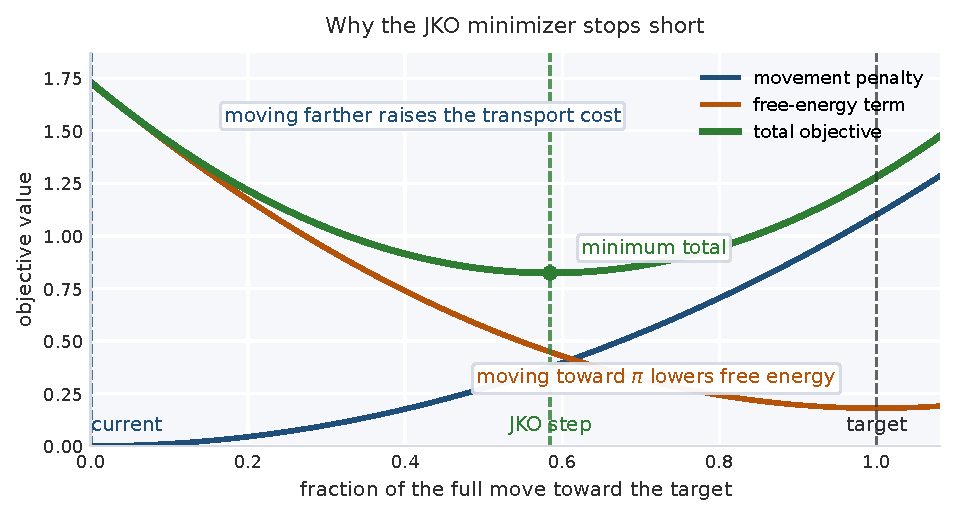
\includegraphics[width=0.9\linewidth]{figures/handouts/langevin_entropy_transport/fig_jko_tradeoff}
  \caption{One JKO step balances two competing effects.
  Moving farther toward equilibrium lowers the free-energy term, but it also increases the Wasserstein movement penalty, so the minimizer of the total objective stops at an interior compromise rather than jumping all the way to $\pi$.}
  \label{fig:jko-tradeoff}
\end{figure}

For a time step $h>0$, the JKO update is
\begin{equation}
  \rho_{k+1}
  \in
  \argmin_{\rho\in\mathcal{P}_2(\R^d)}
  \left\{
    \frac{1}{2h}W_2^2(\rho,\rho_k)+\mathcal{F}(\rho)
  \right\}.
  \label{eq:jko-step}
\end{equation}
The first term penalizes moving too far from the current density.
The second rewards lower free energy.
\Cref{fig:jko-tradeoff} is the picture to keep in mind: JKO is not ``jump to the minimizer of $\mathcal{F}$''; it is a one-step compromise between transport cost and dissipation.

\subsection{A Gaussian JKO calculation}
\label{subsec:jko-gaussian}

Take a quadratic target
\[
U(x)=\frac12 x^\top Hx,
\qquad
H\succ 0,
\]
so the equilibrium law is $\pi=\mathcal{N}(0,H^{-1})$.
To see what \eqref{eq:jko-step} is doing, first restrict attention to the translated Gaussian family
\[
\rho_m:=\mathcal{N}(m,H^{-1}),
\qquad
m\in\R^d.
\]
The covariance already matches the target, so only the mean is moving.

\begin{proposition}[Gaussian JKO mean update]
\label{prop:gaussian-jko-mean}
Fix $m_k\in\R^d$ and let $\rho_k=\rho_{m_k}$.
If we minimize the JKO objective \eqref{eq:jko-step} over translated Gaussians $\rho_m$, then
\begin{equation}
  m_{k+1}
  =
  (I_d+hH)^{-1}m_k.
  \label{eq:gaussian-jko-mean}
\end{equation}
Equivalently, the mean follows implicit Euler for the ODE $\dot m=-Hm$.
\end{proposition}

\begin{proof}
All densities $\rho_m$ have the same covariance, so their entropy terms are equal.
By \Cref{prop:free-energy-kl},
\[
\mathcal{F}(\rho_m)-\mathcal{F}(\pi)=D_{\mathrm{KL}}(\rho_m\|\pi).
\]
For Gaussians with common covariance $H^{-1}$,
\[
D_{\mathrm{KL}}(\rho_m\|\pi)=\frac12 m^\top Hm,
\qquad
W_2^2(\rho_m,\rho_{m_k})=\norm{m-m_k}_2^2.
\]
Therefore minimizing \eqref{eq:jko-step} over the translated family is exactly
\[
m_{k+1}
\in
\argmin_{m\in\R^d}
\left\{
\frac{1}{2h}\norm{m-m_k}_2^2+\frac12 m^\top Hm
\right\}.
\]
The first-order condition is
\[
\frac{1}{h}(m_{k+1}-m_k)+Hm_{k+1}=0,
\]
which rearranges to \eqref{eq:gaussian-jko-mean}.%
\end{proof}

This is already a real calculation, not a slogan.
JKO reproduces the correct mean evolution and it does so through an \emph{implicit} step.
That implicit character matters.
If $H=Q\Lambda Q^\top$ with $\Lambda=\mathrm{diag}(\lambda_1,\dots,\lambda_d)$ and $u_k:=Q^\top m_k$, then
\begin{equation}
  u_{k+1,i}
  =
  \frac{1}{1+h\lambda_i}\,u_{k,i},
  \qquad i=1,\dots,d.
  \label{eq:jko-modewise}
\end{equation}
Every mode contracts, and stiffer modes contract more aggressively.
There is no explicit-Euler stability restriction of the form $h<2/\lambda_{\max}$ in this mean calculation.
That is one reason minimizing movements are such a natural analytic tool.

\begin{figure}[t]
  \centering
  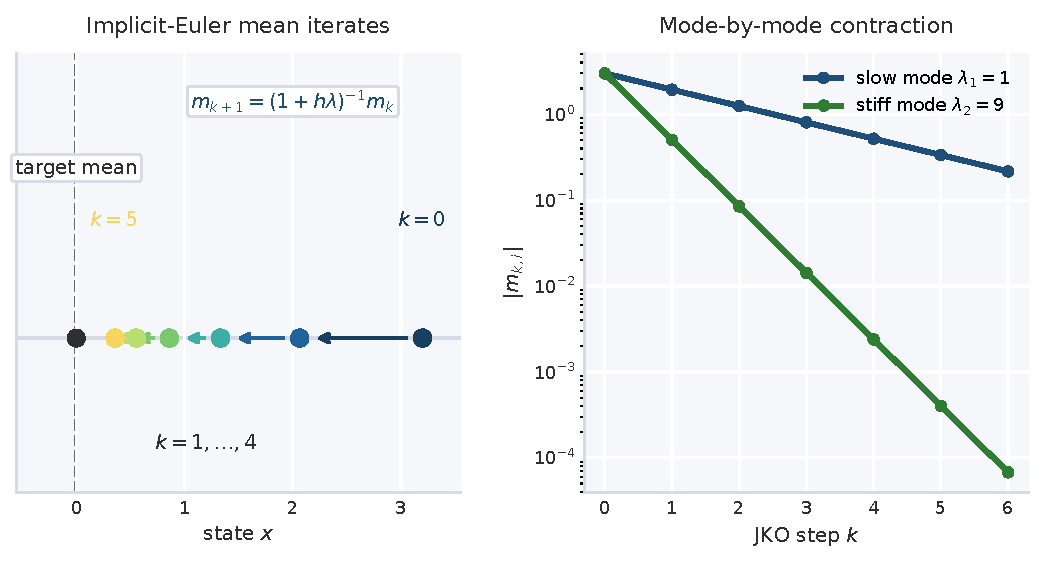
\includegraphics[width=0.9\linewidth]{figures/handouts/langevin_entropy_transport/fig_gaussian_jko_steps}
  \caption{For a quadratic target, restricting JKO to translated Gaussians keeps the covariance fixed and moves only the mean.
  That mean update is exactly implicit Euler, and in diagonal coordinates each mode contracts by $(1+h\lambda_i)^{-1}$, so stiff directions settle faster.}
  \label{fig:gaussian-jko}
\end{figure}

\Cref{fig:gaussian-jko} makes the same point visually.
The left panel shows the mean locations of those translated-Gaussian minimizers.
Because the covariance is fixed inside this restricted family, tracking the means is enough to see the entire update.
The right panel shows the mode-by-mode damping from \eqref{eq:jko-modewise}.

\begin{exercise}[Computing the Gaussian JKO mean step]
\label{ex:gaussian-jko-mean}
Work in the translated Gaussian family from \Cref{prop:gaussian-jko-mean}.
\begin{enumerate}[leftmargin=*]
  \item Show that $W_2^2(\rho_m,\rho_{m_k})=\norm{m-m_k}_2^2$.
  \item Show that $\mathcal{F}(\rho_m)-\mathcal{F}(\pi)=\tfrac12 m^\top Hm$.
  \item Derive \eqref{eq:gaussian-jko-mean} and the mode-by-mode contraction formula \eqref{eq:jko-modewise}.
\end{enumerate}
\end{exercise}
\SolutionBox[16]{%
\begin{enumerate}[leftmargin=*]
  \item Since $\rho_m$ and $\rho_{m_k}$ have the same covariance, the optimal transport is just translation by $m-m_k$, so
  \[
  W_2^2(\rho_m,\rho_{m_k})=\norm{m-m_k}_2^2.
  \]
  \item By \Cref{prop:free-energy-kl},
  \[
  \mathcal{F}(\rho_m)-\mathcal{F}(\pi)=D_{\mathrm{KL}}(\rho_m\|\pi).
  \]
  For Gaussians with equal covariance $H^{-1}$, the KL divergence reduces to the quadratic mean term
  \[
  D_{\mathrm{KL}}(\rho_m\|\pi)=\frac12 m^\top Hm.
  \]
  \item Therefore the JKO objective restricted to translated Gaussians is
  \[
  \Phi(m)=\frac{1}{2h}\norm{m-m_k}_2^2+\frac12 m^\top Hm.
  \]
  Its gradient is
  \[
  \nabla \Phi(m)=\frac{1}{h}(m-m_k)+Hm.
  \]
  Setting this to zero at the minimizer gives
  \[
  \frac{1}{h}(m_{k+1}-m_k)+Hm_{k+1}=0,
  \]
  hence
  \[
  m_{k+1}=(I_d+hH)^{-1}m_k.
  \]
  If $H=Q\Lambda Q^\top$ and $u_k=Q^\top m_k$, then
  \[
  u_{k+1}=Q^\top(I_d+hH)^{-1}Q\,u_k=(I_d+h\Lambda)^{-1}u_k,
  \]
  so each coordinate satisfies
  \[
  u_{k+1,i}=\frac{1}{1+h\lambda_i}u_{k,i}.
  \]
\end{enumerate}%
}

\subsection{The implicit velocity law}
\label{subsec:jko-velocity-law}

The mean calculation shows the basic mechanism in one tractable family, but the full measure-space update has an equally important first-order condition.
If $\rho_{k+1}$ is a smooth positive minimizer of \eqref{eq:jko-step} and $T_{k+1}$ is the optimal transport map from $\rho_{k+1}$ to $\rho_k$, then the Euler--Lagrange condition can be written as
\begin{equation}
  \frac{\operatorname{id}-T_{k+1}}{h}
  =
  -\nabla\bigl(U+\log \rho_{k+1}\bigr)
  \qquad \rho_{k+1}\text{-a.e.}
  \label{eq:jko-euler-lagrange}
\end{equation}
see \citet[\S4.5, Prop.~4.16]{santambrogio_2016_gradient_flows_overview}.
This is exactly the measure-space analogue of the implicit Euler equation
\[
\frac{x_{k+1}-x_k}{h}=-\nabla F(x_{k+1}).
\]
The transport displacement per unit time equals the free-energy velocity, evaluated at the \emph{new} density.

\subsection{The general JKO theorem}
\label{subsec:jko-general-theorem}

The full theorem is much deeper than the Gaussian example, and we do not try to reproduce the compactness proof here.
For our purposes, the conclusion is the key point.

\begin{theorem}[JKO scheme for Fokker--Planck, cited]
\label{thm:jko-general}
In the regular setting treated in \citet[\S4.5, Eq.~(4.13), Prop.~4.14, Prop.~4.19, pp.~37--42]{santambrogio_2016_gradient_flows_overview}, each minimization problem in \eqref{eq:jko-step} is well posed, and as $h\downarrow 0$ the recursive minimizers admit piecewise constant or geodesic interpolants that converge to the solution of the corresponding Fokker--Planck equation with the prescribed initial density.
In this sense, the Fokker--Planck equation is the $W_2$-gradient flow of free energy.
\end{theorem}

The cited proof is written on a compact domain with a $C^1$ confinement potential.
For the Langevin setting on $\R^d$, one imposes the corresponding confinement and integrability assumptions to recover the same minimizing-movement picture.
That theorem is the mathematical heart of the note.
It upgrades the formal continuity-equation picture from \Cref{prop:fokker-planck-continuity} into a precise variational statement: Langevin is not merely a diffusion with invariant law $\pi$; it is the steepest descent of $\mathcal{F}$ in Wasserstein geometry.
The right way to read the theorem is as an infinite-dimensional implicit-Euler convergence statement.
For each fixed $h$, the JKO rule produces a discrete descent path of densities.
As the step size shrinks, those variational steps converge to the actual Fokker--Planck evolution.
So the proximal picture is not just an analogy borrowed from optimization language; it is a literal construction of the PDE.

\section{An exact decay identity}
\label{sec:entropy-dissipation}

JKO identifies the geometry of the flow.
The next step is to compute an exact time derivative.
That is what turns the variational picture into a quantitative convergence argument.

\subsection{The instantaneous decay rate}
\label{subsec:fisher-dissipation}

The quantity that records this instantaneous decay rate is the \emph{relative Fisher information}.
It is defined by
\begin{equation}
  I(\rho\|\pi)
  :=
  \int_{\R^d}
  \norm{\nabla\log\frac{\rho}{\pi}}_2^2\,\rho\,dx.
  \label{eq:relative-fisher}
\end{equation}
Because $\log \pi=-U-\log Z$, this can also be written as
\[
I(\rho\|\pi)
=
\int \norm{\nabla(U+\log\rho)}_2^2\,\rho\,dx.
\]
It measures the squared size of the free-energy slope.

\begin{proposition}[Entropy dissipation identity]
\label{prop:entropy-dissipation}
Let $(\rho_t)_{t\ge 0}$ solve the Langevin Fokker--Planck equation.
Under the smoothness and decay assumptions needed for integration by parts,
\begin{equation}
  \frac{d}{dt}D_{\mathrm{KL}}(\rho_t\|\pi)
  =
  -I(\rho_t\|\pi).
  \label{eq:entropy-dissipation}
\end{equation}
\end{proposition}

\begin{proof}
Using mass conservation, $\int \partial_t \rho_t\,dx=0$, we may differentiate the entropy functional as
\begin{align*}
  \frac{d}{dt}D_{\mathrm{KL}}(\rho_t\|\pi)
  &=
  \int \log\frac{\rho_t}{\pi}\,\partial_t \rho_t\,dx.
\end{align*}
From \Cref{prop:fokker-planck-continuity},
\[
\partial_t \rho_t
=
\nabla\cdot\!\left(\rho_t\nabla\log\frac{\rho_t}{\pi}\right).
\]
Therefore
\begin{align*}
  \frac{d}{dt}D_{\mathrm{KL}}(\rho_t\|\pi)
  &=
  \int \log\frac{\rho_t}{\pi}
  \nabla\cdot\!\left(\rho_t\nabla\log\frac{\rho_t}{\pi}\right)\,dx \\
  &=
  -\int
  \norm{\nabla\log\frac{\rho_t}{\pi}}_2^2
  \rho_t\,dx \\
  &=
  -I(\rho_t\|\pi),
\end{align*}
which is \eqref{eq:entropy-dissipation}.%
\end{proof}

\Cref{prop:entropy-dissipation} is the exact dynamic counterpart of \Cref{prop:free-energy-kl}.
Relative entropy is the gap to equilibrium, and Fisher information is the instantaneous rate at which Langevin closes that gap.

\begin{exercise}[Deriving entropy dissipation]
\label{ex:entropy-dissipation}
Starting from \Cref{eq:fokker-planck-continuity}, prove \Cref{eq:entropy-dissipation}.
Then explain why $I(\rho_t\|\pi)=0$ forces $\rho_t=\pi$ under mild connectedness assumptions.
\end{exercise}
\SolutionBox[14]{%
We begin with
\[
D_{\mathrm{KL}}(\rho_t\|\pi)=\int \rho_t \log\frac{\rho_t}{\pi}\,dx.
\]
Since $\int \partial_t \rho_t\,dx=0$,
\[
\frac{d}{dt}D_{\mathrm{KL}}(\rho_t\|\pi)
=
\int \log\frac{\rho_t}{\pi}\,\partial_t \rho_t\,dx.
\]
Using the continuity-equation form,
\[
\partial_t \rho_t
=
\nabla\cdot\!\left(\rho_t\nabla\log\frac{\rho_t}{\pi}\right),
\]
we obtain
\begin{align*}
\frac{d}{dt}D_{\mathrm{KL}}(\rho_t\|\pi)
&=
\int \log\frac{\rho_t}{\pi}\,
\nabla\cdot\!\left(\rho_t\nabla\log\frac{\rho_t}{\pi}\right)\,dx \\
&=
-\int \norm{\nabla\log\frac{\rho_t}{\pi}}_2^2\,\rho_t\,dx \\
&=
-I(\rho_t\|\pi).
\end{align*}
If $I(\rho_t\|\pi)=0$, then $\nabla\log(\rho_t/\pi)=0$ almost everywhere on the support of $\rho_t$, so $\rho_t/\pi$ is constant on each connected component.
Both densities integrate to $1$, so that constant must be $1$, hence $\rho_t=\pi$ almost everywhere.%
}

\subsection{An exact Ornstein--Uhlenbeck example}
\label{subsec:ou-example}

The entropy dissipation identity is completely explicit for Gaussian targets.
Let
\[
U(x)=\frac12 x^\top Hx,
\qquad
H\succ 0,
\qquad
\pi=\mathcal{N}(0,H^{-1}).
\]
Suppose the initial law is
\[
\rho_0=\mathcal{N}(m_0,H^{-1}),
\]
so the covariance already matches equilibrium.
Then the Langevin diffusion preserves Gaussianity and only the mean moves:
\[
\rho_t=\mathcal{N}(m_t,H^{-1}),
\qquad
m_t=e^{-Ht}m_0.
\]
Writing $m_{0,i}$ in an eigenbasis of $H$ with eigenvalues $\lambda_i$ gives
\begin{equation}
  D_{\mathrm{KL}}(\rho_t\|\pi)
  =
  \frac12\sum_{i=1}^d \lambda_i m_{0,i}^2 e^{-2\lambda_i t},
  \qquad
  I(\rho_t\|\pi)
  =
  \sum_{i=1}^d \lambda_i^2 m_{0,i}^2 e^{-2\lambda_i t}.
  \label{eq:ou-kl-fisher}
\end{equation}
Differentiating the first display immediately yields
\[
\frac{d}{dt}D_{\mathrm{KL}}(\rho_t\|\pi)
=
-I(\rho_t\|\pi).
\]
This example is worth keeping in mind because every later result here collapses to an exact mode-by-mode statement in this quadratic setting.

\section{When decay becomes a uniform rate}
\label{sec:lsi}

Entropy dissipation by itself is only an identity.
It tells us the instantaneous decay rate,
\[
\frac{d}{dt}D_{\mathrm{KL}}(\rho_t\|\pi)=-I(\rho_t\|\pi),
\]
but not whether that rate is uniformly large when the chain is still far from equilibrium.
In principle the Fisher information could be small even while the entropy gap is still substantial.
To turn dissipation into a quantitative rate, we need an inequality that forces a large entropy gap to come with a large slope.
The standard tool is the log-Sobolev inequality, and the Bakry--\'Emery criterion is the curvature condition that often guarantees it.

\subsection{A functional inequality that closes the estimate}
\label{subsec:lsi-decay}

A log-Sobolev inequality compares the entropy gap directly to its dissipation.
Because
\[
I(\rho\|\pi)=\int \norm{\nabla \log(\rho/\pi)(x)}_2^2\,\rho(x)\,dx,
\]
the Fisher information is the squared $L^2(\rho)$ size of the relative log-density gradient.
Geometrically, it measures how sharply the density ratio $\rho/\pi$ is still tilted across space.
The log-Sobolev inequality says that a distribution cannot keep a large free-energy gap while that relative tilt is uniformly tiny.
Equivalently, a large mismatch from equilibrium must leave enough slope for Langevin to keep pushing downhill.

\begin{definition}[Log-Sobolev inequality]
\label{def:lsi}
We say that $\pi$ satisfies a log-Sobolev inequality with constant $\alpha>0$ if
\begin{equation}
  D_{\mathrm{KL}}(\rho\|\pi)
  \le
  \frac{1}{2\alpha}I(\rho\|\pi)
  \qquad
  \text{for every smooth density }\rho.
  \label{eq:lsi}
\end{equation}
\end{definition}

\begin{proposition}[LSI implies exponential KL decay]
\label{prop:lsi-kl-decay}
If $\pi$ satisfies \eqref{eq:lsi} with constant $\alpha>0$, then every sufficiently regular Langevin solution satisfies
\begin{equation}
  D_{\mathrm{KL}}(\rho_t\|\pi)
  \le
  e^{-2\alpha t}D_{\mathrm{KL}}(\rho_0\|\pi).
  \label{eq:kl-exponential-decay}
\end{equation}
\end{proposition}

\begin{proof}
By \Cref{prop:entropy-dissipation},
\[
\frac{d}{dt}D_{\mathrm{KL}}(\rho_t\|\pi)
=
-I(\rho_t\|\pi).
\]
Applying the log-Sobolev inequality at time $t$ gives
\[
I(\rho_t\|\pi)\ge 2\alpha D_{\mathrm{KL}}(\rho_t\|\pi),
\]
hence
\[
\frac{d}{dt}D_{\mathrm{KL}}(\rho_t\|\pi)
\le
-2\alpha D_{\mathrm{KL}}(\rho_t\|\pi).
\]
Gronwall's inequality yields \eqref{eq:kl-exponential-decay}.%
\end{proof}

This is the precise place where ``strong log-concavity implies quantitative mixing'' becomes a theorem.
Once Fisher information dominates entropy, the free-energy gap decays exponentially.
The geometric message is that under an LSI the target has no extended almost-flat directions in which a nonequilibrium density can hide.
If $\rho_t$ still differs substantially from $\pi$, then the relative log-density must still have noticeable slope, so the Fokker--Planck flow cannot stall prematurely.

\subsection{The Gaussian benchmark}
\label{subsec:gaussian-lsi}

For the Gaussian target
\[
\gamma_m(dx)\propto e^{-\frac{m}{2}\norm{x}_2^2}\,dx,
\]
the correct LSI constant is $\alpha=m$.
One way to see that is to invoke the curvature criterion in the next subsection, since $\Hess U=mI_d$.
Inside the translated Gaussian family, the constant is visible exactly:
if $\rho=\mathcal{N}(a,m^{-1}I_d)$, then
\[
D_{\mathrm{KL}}(\rho\|\gamma_m)=\frac{m}{2}\norm{a}_2^2,
\qquad
I(\rho\|\gamma_m)=m^2\norm{a}_2^2,
\]
so equality holds in \eqref{eq:lsi}.
That is a useful sanity check.
The Gaussian measure is not merely an example where LSI is true; it is the model case where the constants are exact.

\subsection{Curvature gives LSI}
\label{subsec:bakry-emery}

The next question is where a bound like \eqref{eq:lsi} comes from.
For strongly log-concave targets, the answer is curvature.
If $U$ bends upward everywhere by at least a fixed quadratic amount, then the measure has no broad flat directions in which entropy can stay large while the free-energy slope becomes tiny.
The Bakry--\'Emery criterion turns that idea into a global log-Sobolev constant.

\begin{theorem}[Bakry--\'Emery criterion, cited]
\label{thm:bakry-emery}
Let $\pi(dx)=Z^{-1}e^{-U(x)}\,dx$ on $\R^d$, where $U\in C^2(\R^d)$ and $Z<\infty$.
If
\begin{equation}
  \Hess U(x)\succeq mI_d
  \qquad\text{for every }x\in\R^d
  \label{eq:bakry-emery-curvature}
\end{equation}
for some $m>0$, then $\pi$ satisfies a log-Sobolev inequality with constant $\alpha=m$.
\end{theorem}

We cite \citet[Thm.~2]{otto_villani_2000_talagrand_lsi} for this form of the theorem.
Historically it is the Bakry--\'Emery curvature condition.
The proof uses $\Gamma_2$-calculus rather than the transport arguments used in the surrounding development, so we do not reproduce it.

The geometric meaning of \eqref{eq:bakry-emery-curvature} is that the ambient space always looks at least as confining as a quadratic well.
If $U$ has a uniform quadratic lower bound on curvature, then the target has no flat directions that allow entropy to linger and no broad corridors in which mass can drift with only a weak restoring force.
Misplaced mass must create a visible change in the relative log-density, so the free-energy slope cannot be tiny unless the entropy gap is already small.
That is exactly what \eqref{eq:lsi} formalizes.
What makes the theorem powerful is that it is global.
The lower Hessian bound is required at every point, not just near the mode, and the conclusion controls every smooth density $\rho$.
One can think of $m$ as a universal restoring-force constant: no matter where mass moves, the landscape is always at least as curved as a quadratic well of curvature $m$.
Bakry--\'Emery says that this geometric fact is enough to force a uniform entropy-dissipation estimate.

\section{From entropy to transport}
\label{sec:entropy-to-transport}

We now have an exponential decay theorem in KL divergence.
For proving convergence, that is already enough.
The reason to keep going is that KL and Wasserstein distance answer different questions.
The KL divergence measures excess free energy, while $W_2$ measures how far the mass of $\rho_t$ still has to move in space to match $\pi$.
That geometric viewpoint is closer to the coupling language of the Sampling unit and the conditioning language of the Optimization unit, so it is worth translating entropy control into transport control as well.

\begin{definition}[Talagrand's $T_2$ inequality]
\label{def:t2}
We say that $\pi$ satisfies $T_2(\alpha)$ if
\begin{equation}
  W_2^2(\rho,\pi)
  \le
  \frac{2}{\alpha}D_{\mathrm{KL}}(\rho\|\pi)
  \qquad
  \text{for every density }\rho.
  \label{eq:t2}
\end{equation}
\end{definition}

\begin{theorem}[Otto--Villani, cited]
\label{thm:otto-villani}
Let $\pi(dx)=Z^{-1}e^{-U(x)}\,dx$ be a probability measure on $\R^d$ with finite second moment, where $U\in C^2(\R^d)$ and
\[
\Hess U(x)\succeq C I_d
\qquad\text{for every }x\in\R^d
\]
for some $C\in\R$.
If $\pi$ satisfies a log-Sobolev inequality with constant $\alpha>0$, then $\pi$ also satisfies $T_2(\alpha)$.
\end{theorem}

This is \citet[Thm.~1]{otto_villani_2000_talagrand_lsi}.
It says that once entropy is controlled, the amount of spatial transport still needed to reach equilibrium is controlled automatically.
That is not obvious a priori because the two quantities measure different kinds of mismatch.
The KL divergence compares density values pointwise, while $W_2$ measures the cost of rearranging mass in space.
The theorem says that an LSI is strong enough to connect them: under sufficient curvature, any large remaining transport cost would itself force a large entropy gap.
So transport control is not an extra ingredient added on top of entropy control; it is a geometric consequence of the same inequality.

\begin{samepage}
\begin{corollary}[Wasserstein decay from LSI]
\label{cor:wasserstein-decay}
Under the hypotheses of \Cref{thm:otto-villani}, every sufficiently regular Langevin solution satisfies
\begin{equation}
  W_2(\rho_t,\pi)
  \le
  \sqrt{\frac{2}{\alpha}}\,
  e^{-\alpha t}
  \sqrt{D_{\mathrm{KL}}(\rho_0\|\pi)}.
  \label{eq:w2-decay}
\end{equation}
\end{corollary}
\end{samepage}

\begin{proof}
Combine \Cref{thm:otto-villani} with \Cref{prop:lsi-kl-decay}:
\[
W_2^2(\rho_t,\pi)
\le
\frac{2}{\alpha}D_{\mathrm{KL}}(\rho_t\|\pi)
\le
\frac{2}{\alpha}e^{-2\alpha t}D_{\mathrm{KL}}(\rho_0\|\pi).
\]
Taking square roots gives \eqref{eq:w2-decay}.%
\end{proof}

For the Gaussian family from \Cref{subsec:gaussian-lsi}, the bridge is exact on translated states:
if $\rho=\mathcal{N}(a,m^{-1}I_d)$ and $\gamma_m=\mathcal{N}(0,m^{-1}I_d)$, then
\[
W_2^2(\rho,\gamma_m)=\norm{a}_2^2=\frac{2}{m}D_{\mathrm{KL}}(\rho\|\gamma_m).
\]
So the LSI-to-$T_2$ story is not merely qualitative.
Its constants are already sharp in the Gaussian model.

\begin{exercise}[From LSI to a Wasserstein bound]
\label{ex:lsi-to-w2}
Assume $\pi$ satisfies LSI$(\alpha)$.
\begin{enumerate}[leftmargin=*]
  \item Use \Cref{prop:entropy-dissipation} to derive \Cref{eq:kl-exponential-decay}.
  \item Combine that with \Cref{eq:t2} to prove \Cref{eq:w2-decay}.
  \item Verify directly in the translated Gaussian family that $T_2(\alpha)$ holds with equality.
\end{enumerate}
\end{exercise}
\SolutionBox[14]{%
\begin{enumerate}[leftmargin=*]
  \item By entropy dissipation,
  \[
  \frac{d}{dt}D_{\mathrm{KL}}(\rho_t\|\pi)=-I(\rho_t\|\pi).
  \]
  The LSI bound gives
  \[
  I(\rho_t\|\pi)\ge 2\alpha D_{\mathrm{KL}}(\rho_t\|\pi),
  \]
  so
  \[
  \frac{d}{dt}D_{\mathrm{KL}}(\rho_t\|\pi)\le -2\alpha D_{\mathrm{KL}}(\rho_t\|\pi).
  \]
  Gronwall yields
  \[
  D_{\mathrm{KL}}(\rho_t\|\pi)\le e^{-2\alpha t}D_{\mathrm{KL}}(\rho_0\|\pi).
  \]
  \item Talagrand's inequality gives
  \[
  W_2^2(\rho_t,\pi)\le \frac{2}{\alpha}D_{\mathrm{KL}}(\rho_t\|\pi).
  \]
  Substituting the KL decay bound,
  \[
  W_2^2(\rho_t,\pi)\le \frac{2}{\alpha}e^{-2\alpha t}D_{\mathrm{KL}}(\rho_0\|\pi),
  \]
  and taking square roots gives \eqref{eq:w2-decay}.
  \item For $\gamma_\alpha=\mathcal{N}(0,\alpha^{-1}I_d)$ and $\rho=\mathcal{N}(a,\alpha^{-1}I_d)$,
  \[
  W_2^2(\rho,\gamma_\alpha)=\norm{a}_2^2
  \]
  because the optimal transport is translation by $a$, while
  \[
  D_{\mathrm{KL}}(\rho\|\gamma_\alpha)=\frac{\alpha}{2}\norm{a}_2^2.
  \]
  Hence
  \[
  W_2^2(\rho,\gamma_\alpha)=\frac{2}{\alpha}D_{\mathrm{KL}}(\rho\|\gamma_\alpha),
  \]
  so $T_2(\alpha)$ is attained exactly on this translated Gaussian family.%
\end{enumerate}
}

\section{Preconditioning and a real posterior}
\label{sec:preconditioning-real-data}

The functional-inequality chain explains why Langevin converges.
The final question is where the constants come from in practice.
For quadratic or locally quadratic targets, the answer is geometric: the relevant rates are the eigenvalues of the preconditioned Hessian.

\subsection{Quadratic targets and the rate matrix}
\label{subsec:preconditioning-quadratic}

Now return to geometry.
Consider the preconditioned overdamped Langevin diffusion
\begin{equation}
  dX_t=-M\nabla U(X_t)\,dt+\sqrt{2M}\,dB_t,
  \label{eq:preconditioned-langevin}
\end{equation}
where $M\succ 0$ is a fixed symmetric positive-definite matrix.
For a quadratic potential centered at $x_\star$,
\[
U(x)=\frac12 (x-x_\star)^\top H(x-x_\star),
\qquad
H\succ 0,
\]
the geometry is again exact.

\begin{proposition}[The relevant rate matrix is $M^{1/2}HM^{1/2}$]
\label{prop:preconditioned-rate-matrix}
Let $Y_t:=M^{-1/2}(X_t-x_\star)$.
Then \eqref{eq:preconditioned-langevin} becomes
\begin{equation}
  dY_t=-A Y_t\,dt+\sqrt{2}\,dB_t,
  \qquad
  A:=M^{1/2}HM^{1/2}.
  \label{eq:preconditioned-ou}
\end{equation}
Hence the mode-by-mode decay rates are the eigenvalues of $A$, not of $H$ alone.
In particular, if $M=H^{-1}$, then $A=I_d$ and all local modes are equalized.
\end{proposition}

\begin{proof}
Write $X_t=x_\star+M^{1/2}Y_t$.
Then
\[
dX_t=M^{1/2}dY_t,
\qquad
\nabla U(X_t)=H(X_t-x_\star)=HM^{1/2}Y_t.
\]
Substituting into \eqref{eq:preconditioned-langevin},
\[
M^{1/2}dY_t=-MHM^{1/2}Y_t\,dt+\sqrt{2M}\,dB_t.
\]
Multiplying by $M^{-1/2}$ gives
\[
dY_t=-M^{1/2}HM^{1/2}Y_t\,dt+\sqrt{2}\,dB_t,
\]
which is \eqref{eq:preconditioned-ou}.%
\end{proof}

The local conclusion is immediate.
Whitening is not mysterious.
It is exactly the choice of $M$ that turns the local quadratic surrogate into an isotropic Ornstein--Uhlenbeck process.

The entropy and transport quantities from earlier sections are also explicit here.
If the transformed process starts from
\[
Y_0\sim \mathcal{N}(m_0,A^{-1}),
\]
then
\[
Y_t\sim \mathcal{N}(e^{-At}m_0,A^{-1}),
\]
so in an eigenbasis of $A$ with eigenvalues $\nu_i$ and coordinates $c_i$ of $m_0$,
\begin{equation}
  D_{\mathrm{KL}}(\rho_t\|\pi)
  =
  \frac12\sum_i \nu_i c_i^2 e^{-2\nu_i t},
  \qquad
  I(\rho_t\|\pi)
  =
  \sum_i \nu_i^2 c_i^2 e^{-2\nu_i t},
  \qquad
  W_2^2(\rho_t,\pi)
  =
  \sum_i c_i^2 e^{-2\nu_i t}.
  \label{eq:preconditioned-decay-formulas}
\end{equation}
When $M=H^{-1}$, all $\nu_i$ become $1$, so every mode decays on the same time scale.

\begin{figure}[t]
  \centering
  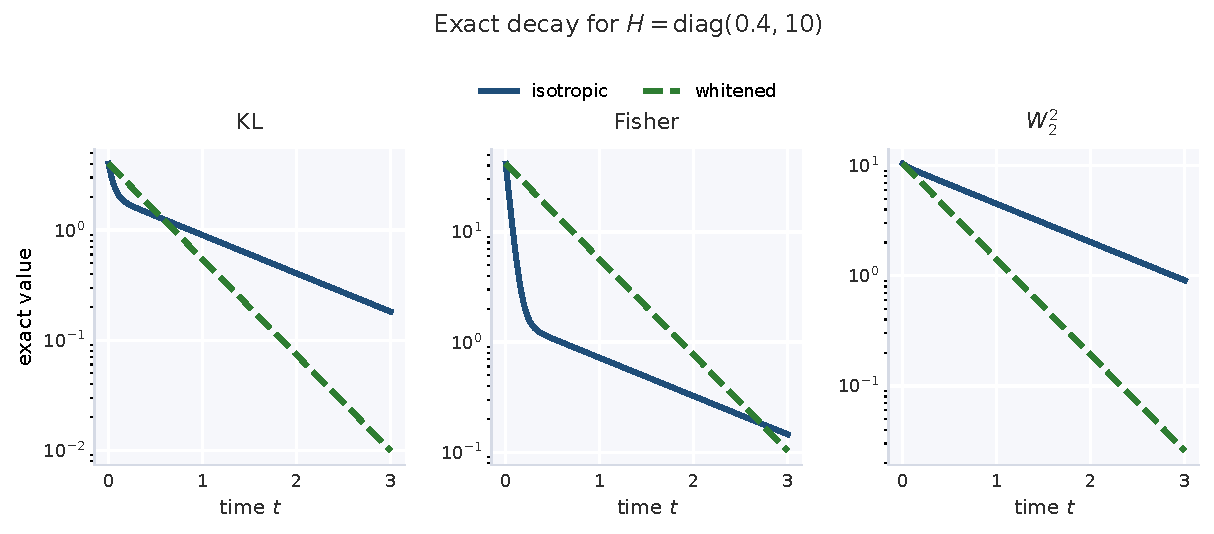
\includegraphics[width=0.95\linewidth]{figures/handouts/langevin_entropy_transport/fig_gaussian_decay_preconditioning}
  \caption{For an anisotropic Gaussian target, KL, Fisher information, and $W_2^2$ decay exactly under the local Ornstein--Uhlenbeck dynamics.
  Whitening turns the rate matrix into the identity and removes the slow mode.}
  \label{fig:gaussian-preconditioning}
\end{figure}

\Cref{fig:gaussian-preconditioning} shows \eqref{eq:preconditioned-decay-formulas} for a simple two-dimensional quadratic target.
The visual simplification reflects an analytic one.
Whitening changes the exact exponents appearing in every convergence quantity derived above.

\subsection{Bayesian logistic regression on the Problem Set 2 data}
\label{subsec:logistic-real-data}

To keep the real-data example aligned with the notes, we return to the regularized logistic-regression model that runs through the Optimization unit and reappears in Problem Set~2.
The dataset has five predictors and a binary response.
In the optimization material, this model supplied explicit gradients, Hessians, and the MAP/Laplace calculation.
Here the same local quadratic surrogate serves a different purpose: it reveals the local rate matrix seen by overdamped Langevin near the MAP.

Write
\[
\beta=(\beta_0,\beta_1,\dots,\beta_5)^\top,
\qquad
\tilde x_i=(1,x_{i1},\dots,x_{i5})^\top.
\]
We also keep the same isotropic Gaussian prior as in Problem Set~2,
\[
\beta\sim \mathcal{N}(0,100 I_6),
\]
so the prior precision is $\lambda=0.01$.
The negative log posterior is
\begin{equation}
  U(\beta)
  =
  \sum_{i=1}^n \Bigl[\log\!\bigl(1+e^{\tilde x_i^\top\beta}\bigr)-y_i \tilde x_i^\top\beta\Bigr]
  +
  \frac{\lambda}{2}\norm{\beta}_2^2.
  \label{eq:logistic-posterior}
\end{equation}
If $p_i(\beta)=\sigma(\tilde x_i^\top\beta)$ with $\sigma(t)=1/(1+e^{-t})$, then
\[
\nabla U(\beta)=X^\top(p(\beta)-y)+\lambda\beta,
\qquad
\Hess U(\beta)=X^\top W(\beta)X+\lambda I_6,
\]
where $W(\beta)$ is diagonal with entries $p_i(\beta)(1-p_i(\beta))$.

We compute the MAP estimate $\beta_{\mathrm{MAP}}$ numerically and use the Hessian
\[
H_{\mathrm{MAP}}:=\Hess U(\beta_{\mathrm{MAP}})
\]
as a local Gaussian surrogate.
This is exactly the Laplace approximation, and we use it only locally.
The claim is not that the posterior is globally Gaussian.
The claim is that the Hessian near the MAP reveals which local preconditioner equalizes the quadratic surrogate.

\begin{figure}[t]
  \centering
  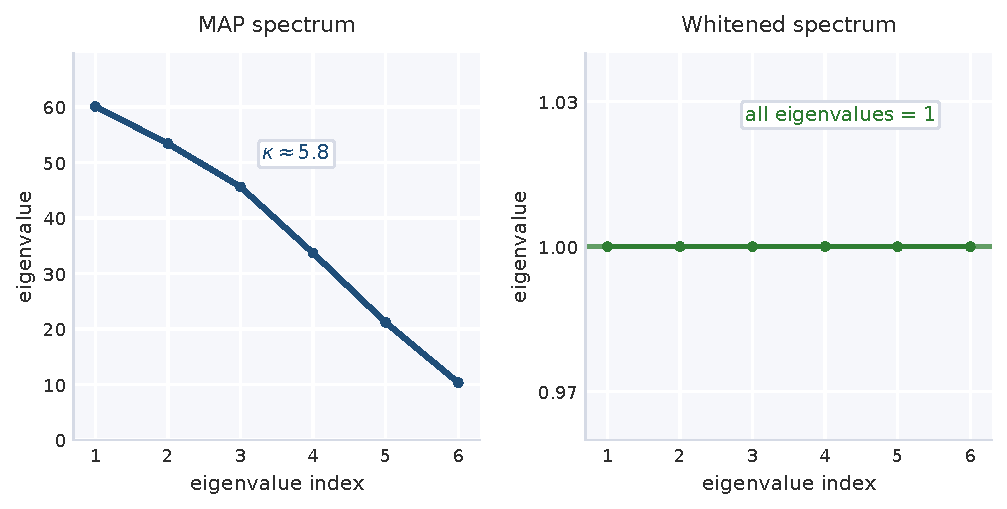
\includegraphics[width=0.92\linewidth]{figures/handouts/langevin_entropy_transport/fig_logistic_hessian_spectrum}
  \caption{The Problem Set 2 Bayesian logistic posterior has a nontrivial MAP Hessian spectrum.
  Whitening with $H_{\mathrm{MAP}}^{-1/2}$ collapses the local spectrum to $1$.}
  \label{fig:logistic-spectrum}
\end{figure}

\Cref{fig:logistic-spectrum} shows the full Hessian spectrum.
The raw local condition number is about $5.8$.
That is not extreme, but it is large enough to make the soft/stiff splitting visible in a familiar course example.
That spectrum is the continuous-time Langevin analogue of the conditioning language from the Optimization unit and the Sampling unit's gradient-based MCMC subsection.

\begin{figure}[t]
  \centering
  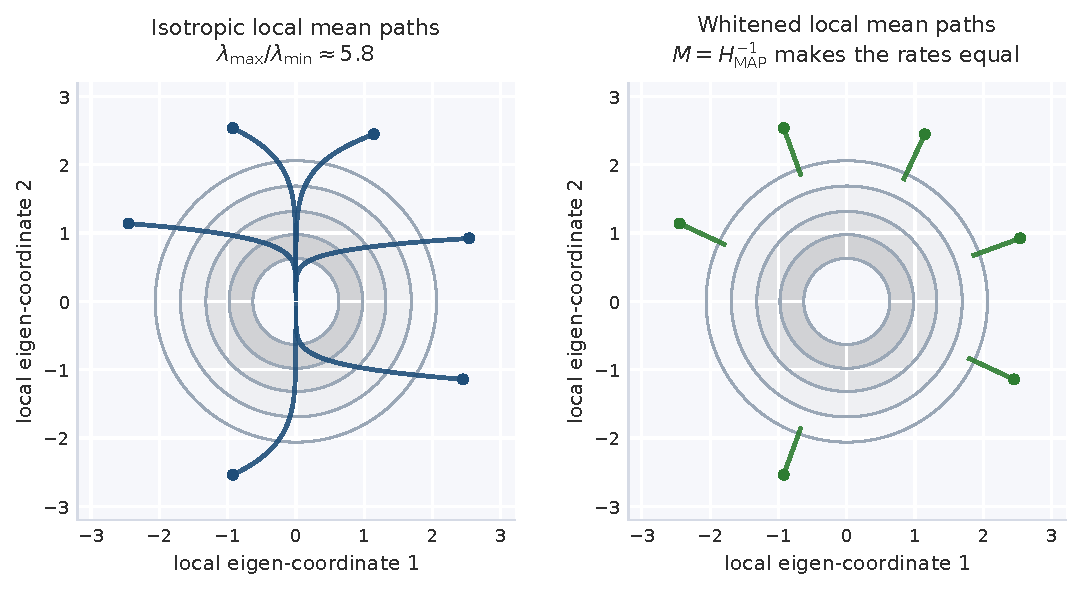
\includegraphics[width=0.92\linewidth]{figures/handouts/langevin_entropy_transport/fig_logistic_laplace_trajectories}
  \caption{The softest/stiffest eigenspace of the Laplace surrogate around the MAP.
  Without preconditioning, local mean paths pinch first along the stiff direction and only later move along the soft direction; local whitening equalizes the contraction rates.}
  \label{fig:logistic-trajectories}
\end{figure}

\Cref{fig:logistic-trajectories} turns the spectrum into a local picture.
Because this model has only six parameters, the figure uses the softest and stiffest eigendirections directly.
The message is the same in either case.
Without preconditioning, the local mean paths collapse first in the stiff direction while progress in the soft direction lags behind.
With $M=H_{\mathrm{MAP}}^{-1}$, the local quadratic surrogate has balanced rates.

This is the right closing connection to the course's conditioning language.
For overdamped Langevin, preconditioning changes the exact rate matrix controlling entropy dissipation and transport contraction.
The same local Hessian picture is what later makes mass-matrix choices matter in the Augmented-state sampling unit's HMC/NUTS development.

\begin{exercise}[Reading the local Hessian geometry]
\label{ex:logistic-preconditioner}
Use \Cref{prop:preconditioned-rate-matrix}, \Cref{fig:logistic-spectrum}, and \Cref{fig:logistic-trajectories}.
\begin{enumerate}[leftmargin=*]
  \item Explain why a spread in the eigenvalues of $H_{\mathrm{MAP}}$ produces multiple local mixing time scales for isotropic Langevin.
  \item Show that choosing $M=H_{\mathrm{MAP}}^{-1}$ makes the local rate matrix equal to the identity.
  \item Why is $H_{\mathrm{MAP}}^{-1}$ the natural quadratic preconditioner, up to an overall scalar factor?
\end{enumerate}
\end{exercise}
\SolutionBox[14]{%
\begin{enumerate}[leftmargin=*]
  \item In the quadratic surrogate, isotropic Langevin corresponds to $M=I_d$, so the local rate matrix is just $H_{\mathrm{MAP}}$.
  Its eigenvalues are the mode-by-mode contraction rates.
  If those eigenvalues vary widely, some directions equilibrate quickly while others remain slow, creating multiple local time scales.
  \item By \Cref{prop:preconditioned-rate-matrix},
  \[
  A=M^{1/2}H_{\mathrm{MAP}}M^{1/2}.
  \]
  Setting $M=H_{\mathrm{MAP}}^{-1}$ gives
  \[
  A=H_{\mathrm{MAP}}^{-1/2}H_{\mathrm{MAP}}H_{\mathrm{MAP}}^{-1/2}=I_d.
  \]
  So all local contraction rates become $1$.
  \item If the goal is to equalize the quadratic modes, then we want $A$ to be proportional to the identity.
  That means
  \[
  M^{1/2}H_{\mathrm{MAP}}M^{1/2}=cI_d
  \]
  for some scalar $c>0$, which is equivalent to
  \[
  M=c\,H_{\mathrm{MAP}}^{-1}.
  \]
  Thus $H_{\mathrm{MAP}}^{-1}$ is the natural local quadratic preconditioner, with any extra scalar factor only changing the overall time scale.%
\end{enumerate}
}

There is also a discrete-time algorithmic payoff.
Once one has an LSI and enough smoothness, these continuous-time decay arguments feed directly into nonasymptotic ULA theory; see \citet[\S3.1, Thm.~1]{vempala_wibisono_2019_ula_isoperimetry}.
The point of that cited result is not that Euler discretization exactly preserves the diffusion analysis.
Rather, good continuous-time geometry survives discretization up to a controlled error, so the same inequalities lead to quantitative bounds for an actual algorithm.
The course-level synthesis is now clear.
Free energy is the Lyapunov functional, JKO is the proximal structure, Fisher information supplies dissipation, LSI turns dissipation into a uniform rate, Talagrand converts that rate into transport control, and preconditioning changes the constants by changing the local geometry.
Carried back to the main notes, this is the optimization story returning in measure space: descent becomes entropy dissipation, proximal structure becomes JKO, and conditioning still determines which directions are easy and which are slow.

\bibliographystyle{plainnat}
\makeatletter
\begingroup
\let\input@path\@empty
\IfFileExists{references.bib}{%
  \gdef\stat221bibpath{references}%
}{%
  \IfFileExists{../references.bib}{%
    \gdef\stat221bibpath{../references}%
  }{%
    \gdef\stat221bibpath{../../references}%
  }%
}
\endgroup
\makeatother
\bibliography{\stat221bibpath}

\end{document}
"
%   (Low-level direct build: if you invoke latexmk manually, set -jobname to the
%    titled output so the compiled PDF matches the standard naming scheme.)
\newif\ifshowsolutions
\showsolutionsfalse
\ifdefined\STATshowsolutions
  \showsolutionstrue
\fi
\ifcsname STAT221SOLUTIONS\endcsname
  \showsolutionstrue
\fi

% Solutions/workspace boxes (controlled by \ifshowsolutions).
% Usage: \SolutionBox[<workspace lines>]{<solution body>}
\newcommand{\SolutionBox}[2][10]{%
  \ifshowsolutions
    \begin{tcolorbox}[stat221panelgray,title={Solution}]
    #2
    \end{tcolorbox}
  \else
    \begin{tcolorbox}[stat221panelgray,unbreakable,title={Workspace}]
    \vspace{#1\baselineskip}
    \end{tcolorbox}
  \fi
}

\title{How do entropy and transport control Langevin convergence?}
\author{}
\date{}

\begin{document}
\maketitle

\section[Entropy, transport, and Langevin]{How do entropy and transport control Langevin convergence?}
\label{sec:langevin-handout-opening}

This handout takes one question from the Sampling unit and studies it in continuous time: how fast does the overdamped Langevin law approach equilibrium, and which geometric assumptions control that rate?
The diffusion itself is
\[
dX_t=-\nabla U(X_t)\,dt+\sqrt{2}\,dB_t,
\]
with stationary law
\[
\pi(x)=Z^{-1}e^{-U(x)}.
\]
Here $Z=\int_{\R^d} e^{-U(x)}\,dx$ is assumed finite, and the evolving object is the law $\rho_t=\mathcal{L}(X_t)$ when $X_0$ does not start from equilibrium.
The main quantities will be the free-energy gap, its dissipation along the Langevin flow, and the transport inequalities that turn dissipation into quantitative convergence.

This viewpoint extends the Sampling unit's gradient-based MCMC subsection, reuses the Optimization unit's language of objectives, proximal structure, and conditioning in measure space, and feeds directly into the Augmented-state sampling unit.
There the same local geometry drives HMC and NUTS through momentum-carrying trajectories rather than one-step Langevin corrections.

There is also a concrete geometric reason to care.
For a quadratic target
\[
U(x)=\frac12 x^\top Hx,
\]
every mode in an eigenbasis of $H$ relaxes at its own exponential rate.
If $H$ is poorly conditioned, then one slow direction controls the last stage of convergence even when the other directions have already equilibrated.
So even in the friendliest Gaussian case, convergence is already controlled by geometry.
The rest of the note develops the general version of that picture:
we identify a free-energy gap to equilibrium, compute its dissipation along the Langevin flow, convert that dissipation into explicit entropy and transport rates, and then read off how preconditioning changes the governing matrix in quadratic and locally quadratic models.

Throughout we work in the smooth, rapidly decaying setting when we differentiate under the integral sign or integrate by parts.
Those formal calculations are the right ones, and the cited theorems extend them to broader classes of densities.

\section{A notion of distance to equilibrium}
\label{sec:free-energy-fokker-planck}

The first task is to identify the right notion of distance to equilibrium.
For Langevin, the natural candidate is not Euclidean distance between points but a functional on densities.
The standard object here is the free-energy gap, and the corresponding density evolution is governed by the Fokker--Planck equation.

\subsection{Relative entropy is a free-energy gap}
\label{subsec:free-energy-gap}

Fix a potential $U:\R^d\to\R$ and define the target density
\[
\pi(x)=Z^{-1}e^{-U(x)},
\qquad
Z=\int_{\R^d} e^{-U(x)}\,dx.
\]
For a probability density $\rho$ we define the free energy
\begin{equation}
  \mathcal{F}(\rho)
  :=
  \int_{\R^d} U(x)\rho(x)\,dx
  +
  \int_{\R^d} \rho(x)\log \rho(x)\,dx.
  \label{eq:free-energy-definition}
\end{equation}
The first term is potential energy.
The second is minus the Shannon entropy, so $\mathcal{F}$ is the natural energy--entropy tradeoff for Langevin diffusion.

\begin{proposition}[Relative entropy equals the free-energy gap]
\label{prop:free-energy-kl}
For every probability density $\rho$ with finite free energy,
\begin{equation}
  D_{\mathrm{KL}}(\rho\|\pi)
  =
  \mathcal{F}(\rho)-\mathcal{F}(\pi).
  \label{eq:free-energy-gap}
\end{equation}
In particular,
\[
\mathcal{F}(\pi)=-\log Z,
\]
so minimizing free energy is the same as minimizing relative entropy to $\pi$.
\end{proposition}

\begin{proof}
Since $\log \pi(x)=-U(x)-\log Z$,
\begin{align*}
  D_{\mathrm{KL}}(\rho\|\pi)
  &=
  \int \rho(x)\log\frac{\rho(x)}{\pi(x)}\,dx \\
  &=
  \int \rho(x)\log \rho(x)\,dx
  +
  \int U(x)\rho(x)\,dx
  +
  \log Z \\
  &=
  \mathcal{F}(\rho)+\log Z.
\end{align*}
Applying the same identity with $\rho=\pi$ gives
\[
0=D_{\mathrm{KL}}(\pi\|\pi)=\mathcal{F}(\pi)+\log Z,
\]
so $\mathcal{F}(\pi)=-\log Z$.
Substituting this into the first formula yields \eqref{eq:free-energy-gap}.%
\end{proof}

\Cref{prop:free-energy-kl} is the basic dictionary for the rest of the note.
The object that decreases along Langevin is not an ad hoc Lyapunov function.
It is exactly the distance to equilibrium measured in relative entropy.

\begin{exercise}[Deriving the free-energy identity]
\label{ex:free-energy-gap}
Starting from \Cref{eq:free-energy-definition} and $\pi(x)=Z^{-1}e^{-U(x)}$, derive \Cref{eq:free-energy-gap}.
Then show directly that $\pi$ minimizes $\mathcal{F}$ over all densities.
\end{exercise}
\SolutionBox[12]{%
We expand the logarithm of the target:
\[
\log \pi(x)=-U(x)-\log Z.
\]
Therefore
\begin{align*}
  D_{\mathrm{KL}}(\rho\|\pi)
  &=
  \int \rho(x)\log\frac{\rho(x)}{\pi(x)}\,dx \\
  &=
  \int \rho(x)\log \rho(x)\,dx
  +
  \int U(x)\rho(x)\,dx
  +
  \log Z \\
  &=
  \mathcal{F}(\rho)+\log Z.
\end{align*}
Setting $\rho=\pi$ gives
\[
0=D_{\mathrm{KL}}(\pi\|\pi)=\mathcal{F}(\pi)+\log Z,
\]
so $\mathcal{F}(\pi)=-\log Z$, hence
\[
D_{\mathrm{KL}}(\rho\|\pi)=\mathcal{F}(\rho)-\mathcal{F}(\pi).
\]
Because relative entropy is always nonnegative and vanishes only when $\rho=\pi$ almost everywhere, $\pi$ is the unique minimizer of $\mathcal{F}$.%
}

\subsection{Langevin as a continuity equation}
\label{subsec:fokker-planck-continuity}

The overdamped Langevin diffusion is
\begin{equation}
  dX_t=-\nabla U(X_t)\,dt+\sqrt{2}\,dB_t.
  \label{eq:overdamped-langevin}
\end{equation}
If $\rho_t$ denotes the density of $X_t$, then $\rho_t$ solves the Fokker--Planck equation
\begin{equation}
  \partial_t \rho_t
  =
  \nabla\cdot(\rho_t\nabla U)+\Delta \rho_t.
  \label{eq:fokker-planck-basic}
\end{equation}
The key rewrite is that the diffusion term can be absorbed into the logarithmic derivative of $\rho_t$.

\begin{proposition}[Continuity-equation form of Fokker--Planck]
\label{prop:fokker-planck-continuity}
Assume $\rho_t$ is smooth and strictly positive.
Then \eqref{eq:fokker-planck-basic} can be written as
\begin{equation}
  \partial_t \rho_t
  =
  \nabla\cdot\!\bigl(\rho_t \nabla(U+\log\rho_t)\bigr)
  =
  -\nabla\cdot(\rho_t v_t),
  \label{eq:fokker-planck-continuity}
\end{equation}
with velocity field
\begin{equation}
  v_t
  =
  -\nabla\bigl(U+\log\rho_t\bigr).
  \label{eq:fokker-planck-velocity}
\end{equation}
\end{proposition}

\begin{proof}
Because $\rho_t>0$,
\[
\Delta \rho_t
=
\nabla\cdot(\nabla \rho_t)
=
\nabla\cdot\!\bigl(\rho_t\nabla\log\rho_t\bigr).
\]
Substituting this into \eqref{eq:fokker-planck-basic} gives
\[
\partial_t \rho_t
=
\nabla\cdot\!\bigl(\rho_t\nabla U\bigr)
+
\nabla\cdot\!\bigl(\rho_t\nabla\log\rho_t\bigr)
=
\nabla\cdot\!\bigl(\rho_t\nabla(U+\log\rho_t)\bigr).
\]
Defining $v_t$ by \eqref{eq:fokker-planck-velocity} yields the continuity equation in \eqref{eq:fokker-planck-continuity}.%
\end{proof}

The field $U+\log \rho_t$ is the first variation of free energy, up to an irrelevant additive constant.
So \Cref{prop:fokker-planck-continuity} says that mass moves downhill in free energy.
What it does not yet give is a one-step rule.
If we freeze time and ask which nearby density should count as the next descent step, we need to say how expensive it is to move one probability law to another.
That is the role of the JKO scheme.

\section{A variational one-step descent rule}
\label{sec:jko}

Free energy tells us what should decrease, but we still need a rule for how to choose the next density from the current one.
Starting from $\rho_k$, we want a new law that lowers $\mathcal{F}$ without moving mass arbitrarily far in a single step.
The Jordan--Kinderlehrer--Otto (JKO) construction is the variational rule that makes that tradeoff precise.

The analogy from Euclidean optimization is the proximal form of implicit Euler.
For the ODE $\dot x=-\nabla F(x)$,
\[
x_{k+1}\in\argmin_x \frac{1}{2h}\norm{x-x_k}_2^2+F(x).
\]
The JKO step does the same thing for densities.
It replaces the Euclidean quadratic penalty by a transport penalty between probability measures.
This is the point where the optimization and sampling viewpoints literally meet.
The same implicit-step logic used to stabilize descent methods in optimization becomes a rule for evolving \emph{laws} in sampling, with Wasserstein distance replacing Euclidean distance and free energy replacing the objective function.

\begin{figure}[t]
  \centering
  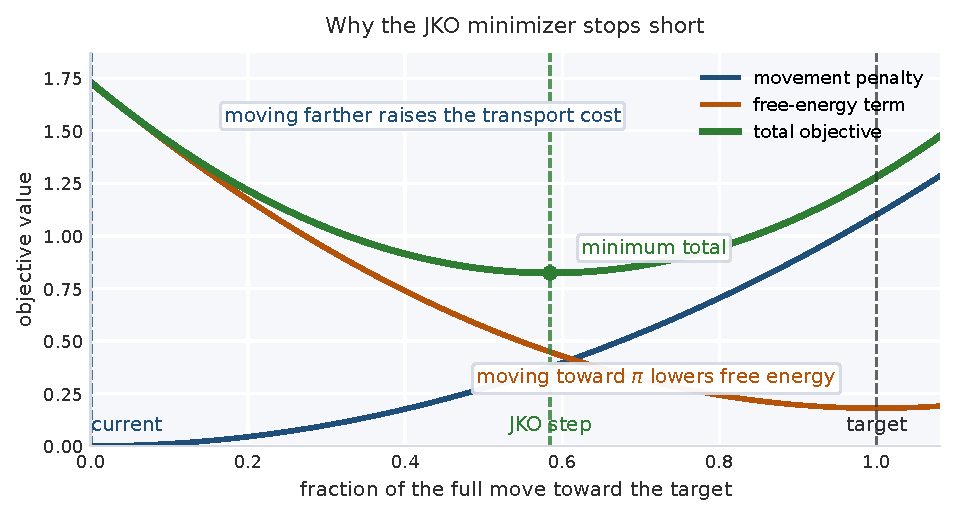
\includegraphics[width=0.9\linewidth]{figures/handouts/langevin_entropy_transport/fig_jko_tradeoff}
  \caption{One JKO step balances two competing effects.
  Moving farther toward equilibrium lowers the free-energy term, but it also increases the Wasserstein movement penalty, so the minimizer of the total objective stops at an interior compromise rather than jumping all the way to $\pi$.}
  \label{fig:jko-tradeoff}
\end{figure}

For a time step $h>0$, the JKO update is
\begin{equation}
  \rho_{k+1}
  \in
  \argmin_{\rho\in\mathcal{P}_2(\R^d)}
  \left\{
    \frac{1}{2h}W_2^2(\rho,\rho_k)+\mathcal{F}(\rho)
  \right\}.
  \label{eq:jko-step}
\end{equation}
The first term penalizes moving too far from the current density.
The second rewards lower free energy.
\Cref{fig:jko-tradeoff} is the picture to keep in mind: JKO is not ``jump to the minimizer of $\mathcal{F}$''; it is a one-step compromise between transport cost and dissipation.

\subsection{A Gaussian JKO calculation}
\label{subsec:jko-gaussian}

Take a quadratic target
\[
U(x)=\frac12 x^\top Hx,
\qquad
H\succ 0,
\]
so the equilibrium law is $\pi=\mathcal{N}(0,H^{-1})$.
To see what \eqref{eq:jko-step} is doing, first restrict attention to the translated Gaussian family
\[
\rho_m:=\mathcal{N}(m,H^{-1}),
\qquad
m\in\R^d.
\]
The covariance already matches the target, so only the mean is moving.

\begin{proposition}[Gaussian JKO mean update]
\label{prop:gaussian-jko-mean}
Fix $m_k\in\R^d$ and let $\rho_k=\rho_{m_k}$.
If we minimize the JKO objective \eqref{eq:jko-step} over translated Gaussians $\rho_m$, then
\begin{equation}
  m_{k+1}
  =
  (I_d+hH)^{-1}m_k.
  \label{eq:gaussian-jko-mean}
\end{equation}
Equivalently, the mean follows implicit Euler for the ODE $\dot m=-Hm$.
\end{proposition}

\begin{proof}
All densities $\rho_m$ have the same covariance, so their entropy terms are equal.
By \Cref{prop:free-energy-kl},
\[
\mathcal{F}(\rho_m)-\mathcal{F}(\pi)=D_{\mathrm{KL}}(\rho_m\|\pi).
\]
For Gaussians with common covariance $H^{-1}$,
\[
D_{\mathrm{KL}}(\rho_m\|\pi)=\frac12 m^\top Hm,
\qquad
W_2^2(\rho_m,\rho_{m_k})=\norm{m-m_k}_2^2.
\]
Therefore minimizing \eqref{eq:jko-step} over the translated family is exactly
\[
m_{k+1}
\in
\argmin_{m\in\R^d}
\left\{
\frac{1}{2h}\norm{m-m_k}_2^2+\frac12 m^\top Hm
\right\}.
\]
The first-order condition is
\[
\frac{1}{h}(m_{k+1}-m_k)+Hm_{k+1}=0,
\]
which rearranges to \eqref{eq:gaussian-jko-mean}.%
\end{proof}

This is already a real calculation, not a slogan.
JKO reproduces the correct mean evolution and it does so through an \emph{implicit} step.
That implicit character matters.
If $H=Q\Lambda Q^\top$ with $\Lambda=\mathrm{diag}(\lambda_1,\dots,\lambda_d)$ and $u_k:=Q^\top m_k$, then
\begin{equation}
  u_{k+1,i}
  =
  \frac{1}{1+h\lambda_i}\,u_{k,i},
  \qquad i=1,\dots,d.
  \label{eq:jko-modewise}
\end{equation}
Every mode contracts, and stiffer modes contract more aggressively.
There is no explicit-Euler stability restriction of the form $h<2/\lambda_{\max}$ in this mean calculation.
That is one reason minimizing movements are such a natural analytic tool.

\begin{figure}[t]
  \centering
  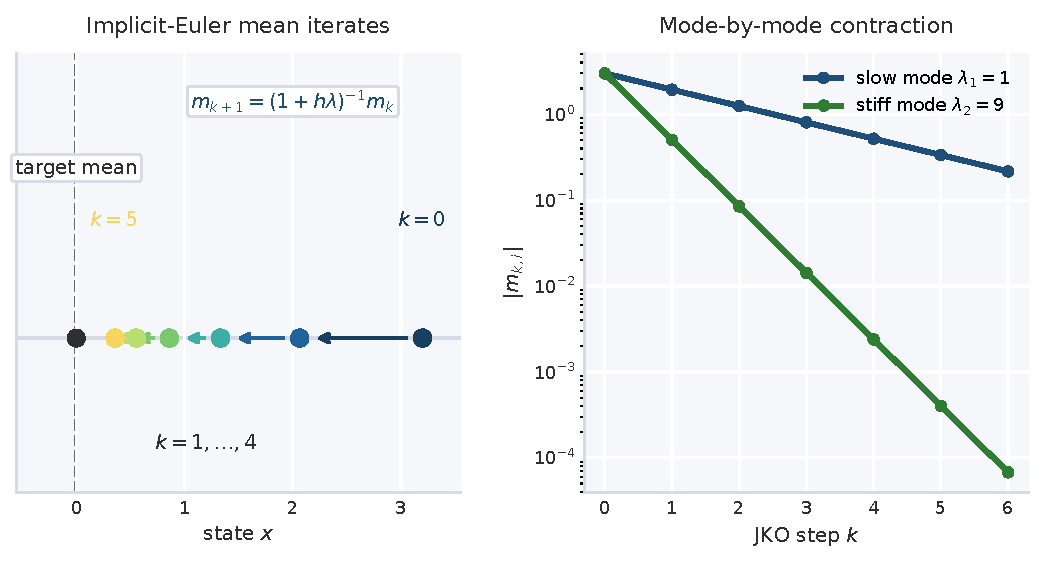
\includegraphics[width=0.9\linewidth]{figures/handouts/langevin_entropy_transport/fig_gaussian_jko_steps}
  \caption{For a quadratic target, restricting JKO to translated Gaussians keeps the covariance fixed and moves only the mean.
  That mean update is exactly implicit Euler, and in diagonal coordinates each mode contracts by $(1+h\lambda_i)^{-1}$, so stiff directions settle faster.}
  \label{fig:gaussian-jko}
\end{figure}

\Cref{fig:gaussian-jko} makes the same point visually.
The left panel shows the mean locations of those translated-Gaussian minimizers.
Because the covariance is fixed inside this restricted family, tracking the means is enough to see the entire update.
The right panel shows the mode-by-mode damping from \eqref{eq:jko-modewise}.

\begin{exercise}[Computing the Gaussian JKO mean step]
\label{ex:gaussian-jko-mean}
Work in the translated Gaussian family from \Cref{prop:gaussian-jko-mean}.
\begin{enumerate}[leftmargin=*]
  \item Show that $W_2^2(\rho_m,\rho_{m_k})=\norm{m-m_k}_2^2$.
  \item Show that $\mathcal{F}(\rho_m)-\mathcal{F}(\pi)=\tfrac12 m^\top Hm$.
  \item Derive \eqref{eq:gaussian-jko-mean} and the mode-by-mode contraction formula \eqref{eq:jko-modewise}.
\end{enumerate}
\end{exercise}
\SolutionBox[16]{%
\begin{enumerate}[leftmargin=*]
  \item Since $\rho_m$ and $\rho_{m_k}$ have the same covariance, the optimal transport is just translation by $m-m_k$, so
  \[
  W_2^2(\rho_m,\rho_{m_k})=\norm{m-m_k}_2^2.
  \]
  \item By \Cref{prop:free-energy-kl},
  \[
  \mathcal{F}(\rho_m)-\mathcal{F}(\pi)=D_{\mathrm{KL}}(\rho_m\|\pi).
  \]
  For Gaussians with equal covariance $H^{-1}$, the KL divergence reduces to the quadratic mean term
  \[
  D_{\mathrm{KL}}(\rho_m\|\pi)=\frac12 m^\top Hm.
  \]
  \item Therefore the JKO objective restricted to translated Gaussians is
  \[
  \Phi(m)=\frac{1}{2h}\norm{m-m_k}_2^2+\frac12 m^\top Hm.
  \]
  Its gradient is
  \[
  \nabla \Phi(m)=\frac{1}{h}(m-m_k)+Hm.
  \]
  Setting this to zero at the minimizer gives
  \[
  \frac{1}{h}(m_{k+1}-m_k)+Hm_{k+1}=0,
  \]
  hence
  \[
  m_{k+1}=(I_d+hH)^{-1}m_k.
  \]
  If $H=Q\Lambda Q^\top$ and $u_k=Q^\top m_k$, then
  \[
  u_{k+1}=Q^\top(I_d+hH)^{-1}Q\,u_k=(I_d+h\Lambda)^{-1}u_k,
  \]
  so each coordinate satisfies
  \[
  u_{k+1,i}=\frac{1}{1+h\lambda_i}u_{k,i}.
  \]
\end{enumerate}%
}

\subsection{The implicit velocity law}
\label{subsec:jko-velocity-law}

The mean calculation shows the basic mechanism in one tractable family, but the full measure-space update has an equally important first-order condition.
If $\rho_{k+1}$ is a smooth positive minimizer of \eqref{eq:jko-step} and $T_{k+1}$ is the optimal transport map from $\rho_{k+1}$ to $\rho_k$, then the Euler--Lagrange condition can be written as
\begin{equation}
  \frac{\operatorname{id}-T_{k+1}}{h}
  =
  -\nabla\bigl(U+\log \rho_{k+1}\bigr)
  \qquad \rho_{k+1}\text{-a.e.}
  \label{eq:jko-euler-lagrange}
\end{equation}
see \citet[\S4.5, Prop.~4.16]{santambrogio_2016_gradient_flows_overview}.
This is exactly the measure-space analogue of the implicit Euler equation
\[
\frac{x_{k+1}-x_k}{h}=-\nabla F(x_{k+1}).
\]
The transport displacement per unit time equals the free-energy velocity, evaluated at the \emph{new} density.

\subsection{The general JKO theorem}
\label{subsec:jko-general-theorem}

The full theorem is much deeper than the Gaussian example, and we do not try to reproduce the compactness proof here.
For our purposes, the conclusion is the key point.

\begin{theorem}[JKO scheme for Fokker--Planck, cited]
\label{thm:jko-general}
In the regular setting treated in \citet[\S4.5, Eq.~(4.13), Prop.~4.14, Prop.~4.19, pp.~37--42]{santambrogio_2016_gradient_flows_overview}, each minimization problem in \eqref{eq:jko-step} is well posed, and as $h\downarrow 0$ the recursive minimizers admit piecewise constant or geodesic interpolants that converge to the solution of the corresponding Fokker--Planck equation with the prescribed initial density.
In this sense, the Fokker--Planck equation is the $W_2$-gradient flow of free energy.
\end{theorem}

The cited proof is written on a compact domain with a $C^1$ confinement potential.
For the Langevin setting on $\R^d$, one imposes the corresponding confinement and integrability assumptions to recover the same minimizing-movement picture.
That theorem is the mathematical heart of the note.
It upgrades the formal continuity-equation picture from \Cref{prop:fokker-planck-continuity} into a precise variational statement: Langevin is not merely a diffusion with invariant law $\pi$; it is the steepest descent of $\mathcal{F}$ in Wasserstein geometry.
The right way to read the theorem is as an infinite-dimensional implicit-Euler convergence statement.
For each fixed $h$, the JKO rule produces a discrete descent path of densities.
As the step size shrinks, those variational steps converge to the actual Fokker--Planck evolution.
So the proximal picture is not just an analogy borrowed from optimization language; it is a literal construction of the PDE.

\section{An exact decay identity}
\label{sec:entropy-dissipation}

JKO identifies the geometry of the flow.
The next step is to compute an exact time derivative.
That is what turns the variational picture into a quantitative convergence argument.

\subsection{The instantaneous decay rate}
\label{subsec:fisher-dissipation}

The quantity that records this instantaneous decay rate is the \emph{relative Fisher information}.
It is defined by
\begin{equation}
  I(\rho\|\pi)
  :=
  \int_{\R^d}
  \norm{\nabla\log\frac{\rho}{\pi}}_2^2\,\rho\,dx.
  \label{eq:relative-fisher}
\end{equation}
Because $\log \pi=-U-\log Z$, this can also be written as
\[
I(\rho\|\pi)
=
\int \norm{\nabla(U+\log\rho)}_2^2\,\rho\,dx.
\]
It measures the squared size of the free-energy slope.

\begin{proposition}[Entropy dissipation identity]
\label{prop:entropy-dissipation}
Let $(\rho_t)_{t\ge 0}$ solve the Langevin Fokker--Planck equation.
Under the smoothness and decay assumptions needed for integration by parts,
\begin{equation}
  \frac{d}{dt}D_{\mathrm{KL}}(\rho_t\|\pi)
  =
  -I(\rho_t\|\pi).
  \label{eq:entropy-dissipation}
\end{equation}
\end{proposition}

\begin{proof}
Using mass conservation, $\int \partial_t \rho_t\,dx=0$, we may differentiate the entropy functional as
\begin{align*}
  \frac{d}{dt}D_{\mathrm{KL}}(\rho_t\|\pi)
  &=
  \int \log\frac{\rho_t}{\pi}\,\partial_t \rho_t\,dx.
\end{align*}
From \Cref{prop:fokker-planck-continuity},
\[
\partial_t \rho_t
=
\nabla\cdot\!\left(\rho_t\nabla\log\frac{\rho_t}{\pi}\right).
\]
Therefore
\begin{align*}
  \frac{d}{dt}D_{\mathrm{KL}}(\rho_t\|\pi)
  &=
  \int \log\frac{\rho_t}{\pi}
  \nabla\cdot\!\left(\rho_t\nabla\log\frac{\rho_t}{\pi}\right)\,dx \\
  &=
  -\int
  \norm{\nabla\log\frac{\rho_t}{\pi}}_2^2
  \rho_t\,dx \\
  &=
  -I(\rho_t\|\pi),
\end{align*}
which is \eqref{eq:entropy-dissipation}.%
\end{proof}

\Cref{prop:entropy-dissipation} is the exact dynamic counterpart of \Cref{prop:free-energy-kl}.
Relative entropy is the gap to equilibrium, and Fisher information is the instantaneous rate at which Langevin closes that gap.

\begin{exercise}[Deriving entropy dissipation]
\label{ex:entropy-dissipation}
Starting from \Cref{eq:fokker-planck-continuity}, prove \Cref{eq:entropy-dissipation}.
Then explain why $I(\rho_t\|\pi)=0$ forces $\rho_t=\pi$ under mild connectedness assumptions.
\end{exercise}
\SolutionBox[14]{%
We begin with
\[
D_{\mathrm{KL}}(\rho_t\|\pi)=\int \rho_t \log\frac{\rho_t}{\pi}\,dx.
\]
Since $\int \partial_t \rho_t\,dx=0$,
\[
\frac{d}{dt}D_{\mathrm{KL}}(\rho_t\|\pi)
=
\int \log\frac{\rho_t}{\pi}\,\partial_t \rho_t\,dx.
\]
Using the continuity-equation form,
\[
\partial_t \rho_t
=
\nabla\cdot\!\left(\rho_t\nabla\log\frac{\rho_t}{\pi}\right),
\]
we obtain
\begin{align*}
\frac{d}{dt}D_{\mathrm{KL}}(\rho_t\|\pi)
&=
\int \log\frac{\rho_t}{\pi}\,
\nabla\cdot\!\left(\rho_t\nabla\log\frac{\rho_t}{\pi}\right)\,dx \\
&=
-\int \norm{\nabla\log\frac{\rho_t}{\pi}}_2^2\,\rho_t\,dx \\
&=
-I(\rho_t\|\pi).
\end{align*}
If $I(\rho_t\|\pi)=0$, then $\nabla\log(\rho_t/\pi)=0$ almost everywhere on the support of $\rho_t$, so $\rho_t/\pi$ is constant on each connected component.
Both densities integrate to $1$, so that constant must be $1$, hence $\rho_t=\pi$ almost everywhere.%
}

\subsection{An exact Ornstein--Uhlenbeck example}
\label{subsec:ou-example}

The entropy dissipation identity is completely explicit for Gaussian targets.
Let
\[
U(x)=\frac12 x^\top Hx,
\qquad
H\succ 0,
\qquad
\pi=\mathcal{N}(0,H^{-1}).
\]
Suppose the initial law is
\[
\rho_0=\mathcal{N}(m_0,H^{-1}),
\]
so the covariance already matches equilibrium.
Then the Langevin diffusion preserves Gaussianity and only the mean moves:
\[
\rho_t=\mathcal{N}(m_t,H^{-1}),
\qquad
m_t=e^{-Ht}m_0.
\]
Writing $m_{0,i}$ in an eigenbasis of $H$ with eigenvalues $\lambda_i$ gives
\begin{equation}
  D_{\mathrm{KL}}(\rho_t\|\pi)
  =
  \frac12\sum_{i=1}^d \lambda_i m_{0,i}^2 e^{-2\lambda_i t},
  \qquad
  I(\rho_t\|\pi)
  =
  \sum_{i=1}^d \lambda_i^2 m_{0,i}^2 e^{-2\lambda_i t}.
  \label{eq:ou-kl-fisher}
\end{equation}
Differentiating the first display immediately yields
\[
\frac{d}{dt}D_{\mathrm{KL}}(\rho_t\|\pi)
=
-I(\rho_t\|\pi).
\]
This example is worth keeping in mind because every later result here collapses to an exact mode-by-mode statement in this quadratic setting.

\section{When decay becomes a uniform rate}
\label{sec:lsi}

Entropy dissipation by itself is only an identity.
It tells us the instantaneous decay rate,
\[
\frac{d}{dt}D_{\mathrm{KL}}(\rho_t\|\pi)=-I(\rho_t\|\pi),
\]
but not whether that rate is uniformly large when the chain is still far from equilibrium.
In principle the Fisher information could be small even while the entropy gap is still substantial.
To turn dissipation into a quantitative rate, we need an inequality that forces a large entropy gap to come with a large slope.
The standard tool is the log-Sobolev inequality, and the Bakry--\'Emery criterion is the curvature condition that often guarantees it.

\subsection{A functional inequality that closes the estimate}
\label{subsec:lsi-decay}

A log-Sobolev inequality compares the entropy gap directly to its dissipation.
Because
\[
I(\rho\|\pi)=\int \norm{\nabla \log(\rho/\pi)(x)}_2^2\,\rho(x)\,dx,
\]
the Fisher information is the squared $L^2(\rho)$ size of the relative log-density gradient.
Geometrically, it measures how sharply the density ratio $\rho/\pi$ is still tilted across space.
The log-Sobolev inequality says that a distribution cannot keep a large free-energy gap while that relative tilt is uniformly tiny.
Equivalently, a large mismatch from equilibrium must leave enough slope for Langevin to keep pushing downhill.

\begin{definition}[Log-Sobolev inequality]
\label{def:lsi}
We say that $\pi$ satisfies a log-Sobolev inequality with constant $\alpha>0$ if
\begin{equation}
  D_{\mathrm{KL}}(\rho\|\pi)
  \le
  \frac{1}{2\alpha}I(\rho\|\pi)
  \qquad
  \text{for every smooth density }\rho.
  \label{eq:lsi}
\end{equation}
\end{definition}

\begin{proposition}[LSI implies exponential KL decay]
\label{prop:lsi-kl-decay}
If $\pi$ satisfies \eqref{eq:lsi} with constant $\alpha>0$, then every sufficiently regular Langevin solution satisfies
\begin{equation}
  D_{\mathrm{KL}}(\rho_t\|\pi)
  \le
  e^{-2\alpha t}D_{\mathrm{KL}}(\rho_0\|\pi).
  \label{eq:kl-exponential-decay}
\end{equation}
\end{proposition}

\begin{proof}
By \Cref{prop:entropy-dissipation},
\[
\frac{d}{dt}D_{\mathrm{KL}}(\rho_t\|\pi)
=
-I(\rho_t\|\pi).
\]
Applying the log-Sobolev inequality at time $t$ gives
\[
I(\rho_t\|\pi)\ge 2\alpha D_{\mathrm{KL}}(\rho_t\|\pi),
\]
hence
\[
\frac{d}{dt}D_{\mathrm{KL}}(\rho_t\|\pi)
\le
-2\alpha D_{\mathrm{KL}}(\rho_t\|\pi).
\]
Gronwall's inequality yields \eqref{eq:kl-exponential-decay}.%
\end{proof}

This is the precise place where ``strong log-concavity implies quantitative mixing'' becomes a theorem.
Once Fisher information dominates entropy, the free-energy gap decays exponentially.
The geometric message is that under an LSI the target has no extended almost-flat directions in which a nonequilibrium density can hide.
If $\rho_t$ still differs substantially from $\pi$, then the relative log-density must still have noticeable slope, so the Fokker--Planck flow cannot stall prematurely.

\subsection{The Gaussian benchmark}
\label{subsec:gaussian-lsi}

For the Gaussian target
\[
\gamma_m(dx)\propto e^{-\frac{m}{2}\norm{x}_2^2}\,dx,
\]
the correct LSI constant is $\alpha=m$.
One way to see that is to invoke the curvature criterion in the next subsection, since $\Hess U=mI_d$.
Inside the translated Gaussian family, the constant is visible exactly:
if $\rho=\mathcal{N}(a,m^{-1}I_d)$, then
\[
D_{\mathrm{KL}}(\rho\|\gamma_m)=\frac{m}{2}\norm{a}_2^2,
\qquad
I(\rho\|\gamma_m)=m^2\norm{a}_2^2,
\]
so equality holds in \eqref{eq:lsi}.
That is a useful sanity check.
The Gaussian measure is not merely an example where LSI is true; it is the model case where the constants are exact.

\subsection{Curvature gives LSI}
\label{subsec:bakry-emery}

The next question is where a bound like \eqref{eq:lsi} comes from.
For strongly log-concave targets, the answer is curvature.
If $U$ bends upward everywhere by at least a fixed quadratic amount, then the measure has no broad flat directions in which entropy can stay large while the free-energy slope becomes tiny.
The Bakry--\'Emery criterion turns that idea into a global log-Sobolev constant.

\begin{theorem}[Bakry--\'Emery criterion, cited]
\label{thm:bakry-emery}
Let $\pi(dx)=Z^{-1}e^{-U(x)}\,dx$ on $\R^d$, where $U\in C^2(\R^d)$ and $Z<\infty$.
If
\begin{equation}
  \Hess U(x)\succeq mI_d
  \qquad\text{for every }x\in\R^d
  \label{eq:bakry-emery-curvature}
\end{equation}
for some $m>0$, then $\pi$ satisfies a log-Sobolev inequality with constant $\alpha=m$.
\end{theorem}

We cite \citet[Thm.~2]{otto_villani_2000_talagrand_lsi} for this form of the theorem.
Historically it is the Bakry--\'Emery curvature condition.
The proof uses $\Gamma_2$-calculus rather than the transport arguments used in the surrounding development, so we do not reproduce it.

The geometric meaning of \eqref{eq:bakry-emery-curvature} is that the ambient space always looks at least as confining as a quadratic well.
If $U$ has a uniform quadratic lower bound on curvature, then the target has no flat directions that allow entropy to linger and no broad corridors in which mass can drift with only a weak restoring force.
Misplaced mass must create a visible change in the relative log-density, so the free-energy slope cannot be tiny unless the entropy gap is already small.
That is exactly what \eqref{eq:lsi} formalizes.
What makes the theorem powerful is that it is global.
The lower Hessian bound is required at every point, not just near the mode, and the conclusion controls every smooth density $\rho$.
One can think of $m$ as a universal restoring-force constant: no matter where mass moves, the landscape is always at least as curved as a quadratic well of curvature $m$.
Bakry--\'Emery says that this geometric fact is enough to force a uniform entropy-dissipation estimate.

\section{From entropy to transport}
\label{sec:entropy-to-transport}

We now have an exponential decay theorem in KL divergence.
For proving convergence, that is already enough.
The reason to keep going is that KL and Wasserstein distance answer different questions.
The KL divergence measures excess free energy, while $W_2$ measures how far the mass of $\rho_t$ still has to move in space to match $\pi$.
That geometric viewpoint is closer to the coupling language of the Sampling unit and the conditioning language of the Optimization unit, so it is worth translating entropy control into transport control as well.

\begin{definition}[Talagrand's $T_2$ inequality]
\label{def:t2}
We say that $\pi$ satisfies $T_2(\alpha)$ if
\begin{equation}
  W_2^2(\rho,\pi)
  \le
  \frac{2}{\alpha}D_{\mathrm{KL}}(\rho\|\pi)
  \qquad
  \text{for every density }\rho.
  \label{eq:t2}
\end{equation}
\end{definition}

\begin{theorem}[Otto--Villani, cited]
\label{thm:otto-villani}
Let $\pi(dx)=Z^{-1}e^{-U(x)}\,dx$ be a probability measure on $\R^d$ with finite second moment, where $U\in C^2(\R^d)$ and
\[
\Hess U(x)\succeq C I_d
\qquad\text{for every }x\in\R^d
\]
for some $C\in\R$.
If $\pi$ satisfies a log-Sobolev inequality with constant $\alpha>0$, then $\pi$ also satisfies $T_2(\alpha)$.
\end{theorem}

This is \citet[Thm.~1]{otto_villani_2000_talagrand_lsi}.
It says that once entropy is controlled, the amount of spatial transport still needed to reach equilibrium is controlled automatically.
That is not obvious a priori because the two quantities measure different kinds of mismatch.
The KL divergence compares density values pointwise, while $W_2$ measures the cost of rearranging mass in space.
The theorem says that an LSI is strong enough to connect them: under sufficient curvature, any large remaining transport cost would itself force a large entropy gap.
So transport control is not an extra ingredient added on top of entropy control; it is a geometric consequence of the same inequality.

\begin{samepage}
\begin{corollary}[Wasserstein decay from LSI]
\label{cor:wasserstein-decay}
Under the hypotheses of \Cref{thm:otto-villani}, every sufficiently regular Langevin solution satisfies
\begin{equation}
  W_2(\rho_t,\pi)
  \le
  \sqrt{\frac{2}{\alpha}}\,
  e^{-\alpha t}
  \sqrt{D_{\mathrm{KL}}(\rho_0\|\pi)}.
  \label{eq:w2-decay}
\end{equation}
\end{corollary}
\end{samepage}

\begin{proof}
Combine \Cref{thm:otto-villani} with \Cref{prop:lsi-kl-decay}:
\[
W_2^2(\rho_t,\pi)
\le
\frac{2}{\alpha}D_{\mathrm{KL}}(\rho_t\|\pi)
\le
\frac{2}{\alpha}e^{-2\alpha t}D_{\mathrm{KL}}(\rho_0\|\pi).
\]
Taking square roots gives \eqref{eq:w2-decay}.%
\end{proof}

For the Gaussian family from \Cref{subsec:gaussian-lsi}, the bridge is exact on translated states:
if $\rho=\mathcal{N}(a,m^{-1}I_d)$ and $\gamma_m=\mathcal{N}(0,m^{-1}I_d)$, then
\[
W_2^2(\rho,\gamma_m)=\norm{a}_2^2=\frac{2}{m}D_{\mathrm{KL}}(\rho\|\gamma_m).
\]
So the LSI-to-$T_2$ story is not merely qualitative.
Its constants are already sharp in the Gaussian model.

\begin{exercise}[From LSI to a Wasserstein bound]
\label{ex:lsi-to-w2}
Assume $\pi$ satisfies LSI$(\alpha)$.
\begin{enumerate}[leftmargin=*]
  \item Use \Cref{prop:entropy-dissipation} to derive \Cref{eq:kl-exponential-decay}.
  \item Combine that with \Cref{eq:t2} to prove \Cref{eq:w2-decay}.
  \item Verify directly in the translated Gaussian family that $T_2(\alpha)$ holds with equality.
\end{enumerate}
\end{exercise}
\SolutionBox[14]{%
\begin{enumerate}[leftmargin=*]
  \item By entropy dissipation,
  \[
  \frac{d}{dt}D_{\mathrm{KL}}(\rho_t\|\pi)=-I(\rho_t\|\pi).
  \]
  The LSI bound gives
  \[
  I(\rho_t\|\pi)\ge 2\alpha D_{\mathrm{KL}}(\rho_t\|\pi),
  \]
  so
  \[
  \frac{d}{dt}D_{\mathrm{KL}}(\rho_t\|\pi)\le -2\alpha D_{\mathrm{KL}}(\rho_t\|\pi).
  \]
  Gronwall yields
  \[
  D_{\mathrm{KL}}(\rho_t\|\pi)\le e^{-2\alpha t}D_{\mathrm{KL}}(\rho_0\|\pi).
  \]
  \item Talagrand's inequality gives
  \[
  W_2^2(\rho_t,\pi)\le \frac{2}{\alpha}D_{\mathrm{KL}}(\rho_t\|\pi).
  \]
  Substituting the KL decay bound,
  \[
  W_2^2(\rho_t,\pi)\le \frac{2}{\alpha}e^{-2\alpha t}D_{\mathrm{KL}}(\rho_0\|\pi),
  \]
  and taking square roots gives \eqref{eq:w2-decay}.
  \item For $\gamma_\alpha=\mathcal{N}(0,\alpha^{-1}I_d)$ and $\rho=\mathcal{N}(a,\alpha^{-1}I_d)$,
  \[
  W_2^2(\rho,\gamma_\alpha)=\norm{a}_2^2
  \]
  because the optimal transport is translation by $a$, while
  \[
  D_{\mathrm{KL}}(\rho\|\gamma_\alpha)=\frac{\alpha}{2}\norm{a}_2^2.
  \]
  Hence
  \[
  W_2^2(\rho,\gamma_\alpha)=\frac{2}{\alpha}D_{\mathrm{KL}}(\rho\|\gamma_\alpha),
  \]
  so $T_2(\alpha)$ is attained exactly on this translated Gaussian family.%
\end{enumerate}
}

\section{Preconditioning and a real posterior}
\label{sec:preconditioning-real-data}

The functional-inequality chain explains why Langevin converges.
The final question is where the constants come from in practice.
For quadratic or locally quadratic targets, the answer is geometric: the relevant rates are the eigenvalues of the preconditioned Hessian.

\subsection{Quadratic targets and the rate matrix}
\label{subsec:preconditioning-quadratic}

Now return to geometry.
Consider the preconditioned overdamped Langevin diffusion
\begin{equation}
  dX_t=-M\nabla U(X_t)\,dt+\sqrt{2M}\,dB_t,
  \label{eq:preconditioned-langevin}
\end{equation}
where $M\succ 0$ is a fixed symmetric positive-definite matrix.
For a quadratic potential centered at $x_\star$,
\[
U(x)=\frac12 (x-x_\star)^\top H(x-x_\star),
\qquad
H\succ 0,
\]
the geometry is again exact.

\begin{proposition}[The relevant rate matrix is $M^{1/2}HM^{1/2}$]
\label{prop:preconditioned-rate-matrix}
Let $Y_t:=M^{-1/2}(X_t-x_\star)$.
Then \eqref{eq:preconditioned-langevin} becomes
\begin{equation}
  dY_t=-A Y_t\,dt+\sqrt{2}\,dB_t,
  \qquad
  A:=M^{1/2}HM^{1/2}.
  \label{eq:preconditioned-ou}
\end{equation}
Hence the mode-by-mode decay rates are the eigenvalues of $A$, not of $H$ alone.
In particular, if $M=H^{-1}$, then $A=I_d$ and all local modes are equalized.
\end{proposition}

\begin{proof}
Write $X_t=x_\star+M^{1/2}Y_t$.
Then
\[
dX_t=M^{1/2}dY_t,
\qquad
\nabla U(X_t)=H(X_t-x_\star)=HM^{1/2}Y_t.
\]
Substituting into \eqref{eq:preconditioned-langevin},
\[
M^{1/2}dY_t=-MHM^{1/2}Y_t\,dt+\sqrt{2M}\,dB_t.
\]
Multiplying by $M^{-1/2}$ gives
\[
dY_t=-M^{1/2}HM^{1/2}Y_t\,dt+\sqrt{2}\,dB_t,
\]
which is \eqref{eq:preconditioned-ou}.%
\end{proof}

The local conclusion is immediate.
Whitening is not mysterious.
It is exactly the choice of $M$ that turns the local quadratic surrogate into an isotropic Ornstein--Uhlenbeck process.

The entropy and transport quantities from earlier sections are also explicit here.
If the transformed process starts from
\[
Y_0\sim \mathcal{N}(m_0,A^{-1}),
\]
then
\[
Y_t\sim \mathcal{N}(e^{-At}m_0,A^{-1}),
\]
so in an eigenbasis of $A$ with eigenvalues $\nu_i$ and coordinates $c_i$ of $m_0$,
\begin{equation}
  D_{\mathrm{KL}}(\rho_t\|\pi)
  =
  \frac12\sum_i \nu_i c_i^2 e^{-2\nu_i t},
  \qquad
  I(\rho_t\|\pi)
  =
  \sum_i \nu_i^2 c_i^2 e^{-2\nu_i t},
  \qquad
  W_2^2(\rho_t,\pi)
  =
  \sum_i c_i^2 e^{-2\nu_i t}.
  \label{eq:preconditioned-decay-formulas}
\end{equation}
When $M=H^{-1}$, all $\nu_i$ become $1$, so every mode decays on the same time scale.

\begin{figure}[t]
  \centering
  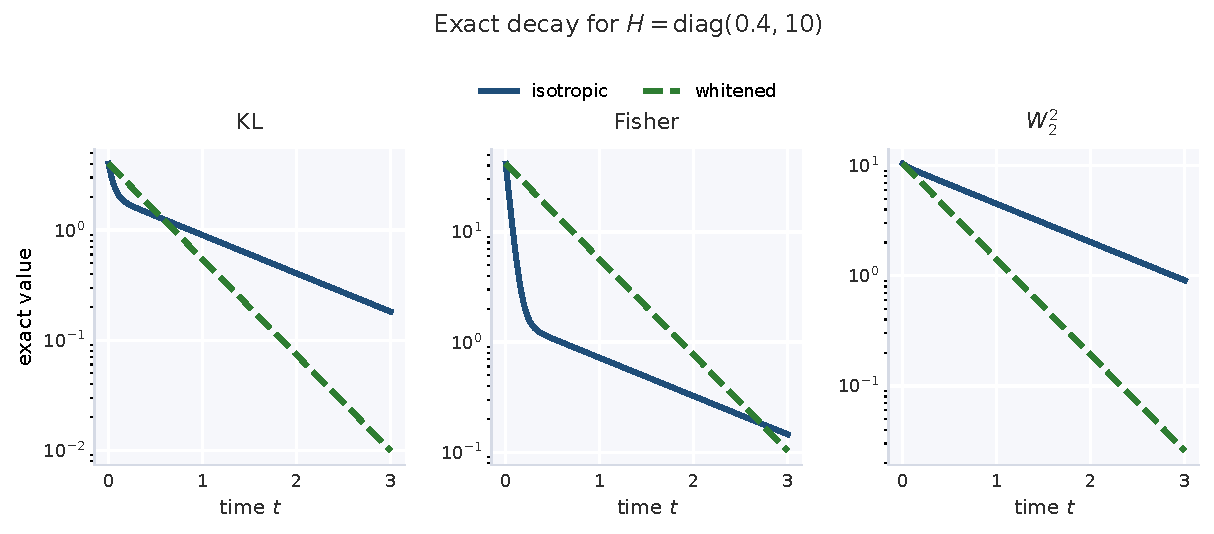
\includegraphics[width=0.95\linewidth]{figures/handouts/langevin_entropy_transport/fig_gaussian_decay_preconditioning}
  \caption{For an anisotropic Gaussian target, KL, Fisher information, and $W_2^2$ decay exactly under the local Ornstein--Uhlenbeck dynamics.
  Whitening turns the rate matrix into the identity and removes the slow mode.}
  \label{fig:gaussian-preconditioning}
\end{figure}

\Cref{fig:gaussian-preconditioning} shows \eqref{eq:preconditioned-decay-formulas} for a simple two-dimensional quadratic target.
The visual simplification reflects an analytic one.
Whitening changes the exact exponents appearing in every convergence quantity derived above.

\subsection{Bayesian logistic regression on the Problem Set 2 data}
\label{subsec:logistic-real-data}

To keep the real-data example aligned with the notes, we return to the regularized logistic-regression model that runs through the Optimization unit and reappears in Problem Set~2.
The dataset has five predictors and a binary response.
In the optimization material, this model supplied explicit gradients, Hessians, and the MAP/Laplace calculation.
Here the same local quadratic surrogate serves a different purpose: it reveals the local rate matrix seen by overdamped Langevin near the MAP.

Write
\[
\beta=(\beta_0,\beta_1,\dots,\beta_5)^\top,
\qquad
\tilde x_i=(1,x_{i1},\dots,x_{i5})^\top.
\]
We also keep the same isotropic Gaussian prior as in Problem Set~2,
\[
\beta\sim \mathcal{N}(0,100 I_6),
\]
so the prior precision is $\lambda=0.01$.
The negative log posterior is
\begin{equation}
  U(\beta)
  =
  \sum_{i=1}^n \Bigl[\log\!\bigl(1+e^{\tilde x_i^\top\beta}\bigr)-y_i \tilde x_i^\top\beta\Bigr]
  +
  \frac{\lambda}{2}\norm{\beta}_2^2.
  \label{eq:logistic-posterior}
\end{equation}
If $p_i(\beta)=\sigma(\tilde x_i^\top\beta)$ with $\sigma(t)=1/(1+e^{-t})$, then
\[
\nabla U(\beta)=X^\top(p(\beta)-y)+\lambda\beta,
\qquad
\Hess U(\beta)=X^\top W(\beta)X+\lambda I_6,
\]
where $W(\beta)$ is diagonal with entries $p_i(\beta)(1-p_i(\beta))$.

We compute the MAP estimate $\beta_{\mathrm{MAP}}$ numerically and use the Hessian
\[
H_{\mathrm{MAP}}:=\Hess U(\beta_{\mathrm{MAP}})
\]
as a local Gaussian surrogate.
This is exactly the Laplace approximation, and we use it only locally.
The claim is not that the posterior is globally Gaussian.
The claim is that the Hessian near the MAP reveals which local preconditioner equalizes the quadratic surrogate.

\begin{figure}[t]
  \centering
  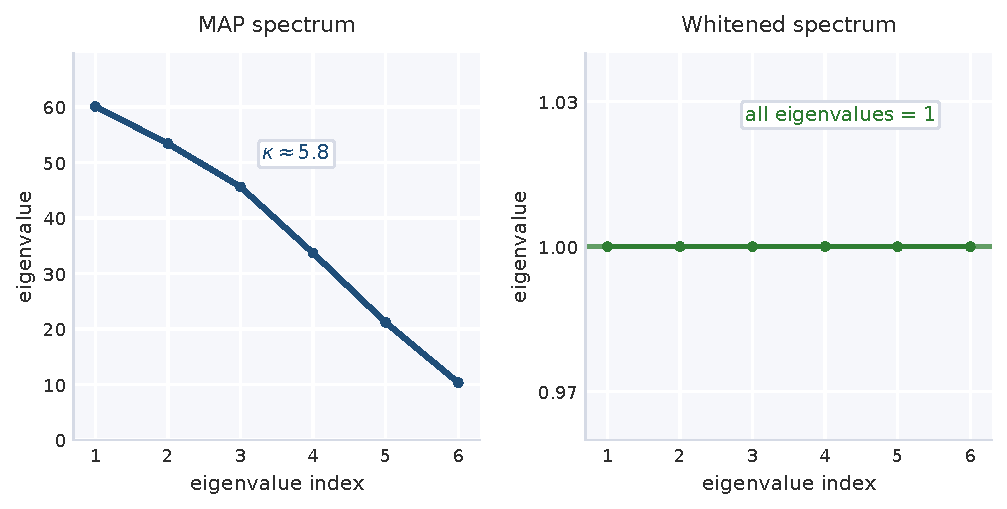
\includegraphics[width=0.92\linewidth]{figures/handouts/langevin_entropy_transport/fig_logistic_hessian_spectrum}
  \caption{The Problem Set 2 Bayesian logistic posterior has a nontrivial MAP Hessian spectrum.
  Whitening with $H_{\mathrm{MAP}}^{-1/2}$ collapses the local spectrum to $1$.}
  \label{fig:logistic-spectrum}
\end{figure}

\Cref{fig:logistic-spectrum} shows the full Hessian spectrum.
The raw local condition number is about $5.8$.
That is not extreme, but it is large enough to make the soft/stiff splitting visible in a familiar course example.
That spectrum is the continuous-time Langevin analogue of the conditioning language from the Optimization unit and the Sampling unit's gradient-based MCMC subsection.

\begin{figure}[t]
  \centering
  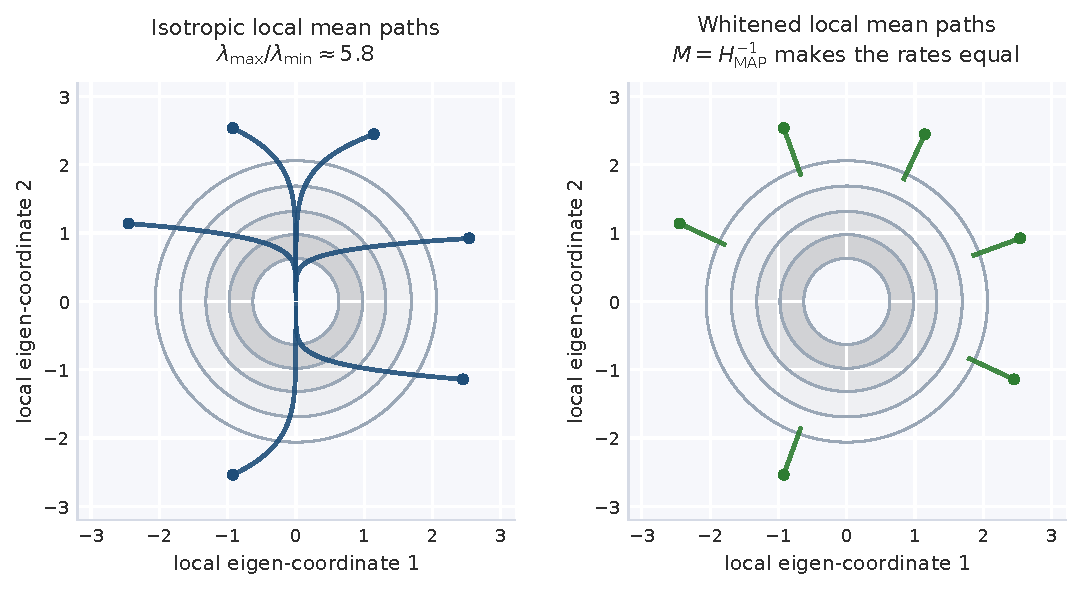
\includegraphics[width=0.92\linewidth]{figures/handouts/langevin_entropy_transport/fig_logistic_laplace_trajectories}
  \caption{The softest/stiffest eigenspace of the Laplace surrogate around the MAP.
  Without preconditioning, local mean paths pinch first along the stiff direction and only later move along the soft direction; local whitening equalizes the contraction rates.}
  \label{fig:logistic-trajectories}
\end{figure}

\Cref{fig:logistic-trajectories} turns the spectrum into a local picture.
Because this model has only six parameters, the figure uses the softest and stiffest eigendirections directly.
The message is the same in either case.
Without preconditioning, the local mean paths collapse first in the stiff direction while progress in the soft direction lags behind.
With $M=H_{\mathrm{MAP}}^{-1}$, the local quadratic surrogate has balanced rates.

This is the right closing connection to the course's conditioning language.
For overdamped Langevin, preconditioning changes the exact rate matrix controlling entropy dissipation and transport contraction.
The same local Hessian picture is what later makes mass-matrix choices matter in the Augmented-state sampling unit's HMC/NUTS development.

\begin{exercise}[Reading the local Hessian geometry]
\label{ex:logistic-preconditioner}
Use \Cref{prop:preconditioned-rate-matrix}, \Cref{fig:logistic-spectrum}, and \Cref{fig:logistic-trajectories}.
\begin{enumerate}[leftmargin=*]
  \item Explain why a spread in the eigenvalues of $H_{\mathrm{MAP}}$ produces multiple local mixing time scales for isotropic Langevin.
  \item Show that choosing $M=H_{\mathrm{MAP}}^{-1}$ makes the local rate matrix equal to the identity.
  \item Why is $H_{\mathrm{MAP}}^{-1}$ the natural quadratic preconditioner, up to an overall scalar factor?
\end{enumerate}
\end{exercise}
\SolutionBox[14]{%
\begin{enumerate}[leftmargin=*]
  \item In the quadratic surrogate, isotropic Langevin corresponds to $M=I_d$, so the local rate matrix is just $H_{\mathrm{MAP}}$.
  Its eigenvalues are the mode-by-mode contraction rates.
  If those eigenvalues vary widely, some directions equilibrate quickly while others remain slow, creating multiple local time scales.
  \item By \Cref{prop:preconditioned-rate-matrix},
  \[
  A=M^{1/2}H_{\mathrm{MAP}}M^{1/2}.
  \]
  Setting $M=H_{\mathrm{MAP}}^{-1}$ gives
  \[
  A=H_{\mathrm{MAP}}^{-1/2}H_{\mathrm{MAP}}H_{\mathrm{MAP}}^{-1/2}=I_d.
  \]
  So all local contraction rates become $1$.
  \item If the goal is to equalize the quadratic modes, then we want $A$ to be proportional to the identity.
  That means
  \[
  M^{1/2}H_{\mathrm{MAP}}M^{1/2}=cI_d
  \]
  for some scalar $c>0$, which is equivalent to
  \[
  M=c\,H_{\mathrm{MAP}}^{-1}.
  \]
  Thus $H_{\mathrm{MAP}}^{-1}$ is the natural local quadratic preconditioner, with any extra scalar factor only changing the overall time scale.%
\end{enumerate}
}

There is also a discrete-time algorithmic payoff.
Once one has an LSI and enough smoothness, these continuous-time decay arguments feed directly into nonasymptotic ULA theory; see \citet[\S3.1, Thm.~1]{vempala_wibisono_2019_ula_isoperimetry}.
The point of that cited result is not that Euler discretization exactly preserves the diffusion analysis.
Rather, good continuous-time geometry survives discretization up to a controlled error, so the same inequalities lead to quantitative bounds for an actual algorithm.
The course-level synthesis is now clear.
Free energy is the Lyapunov functional, JKO is the proximal structure, Fisher information supplies dissipation, LSI turns dissipation into a uniform rate, Talagrand converts that rate into transport control, and preconditioning changes the constants by changing the local geometry.
Carried back to the main notes, this is the optimization story returning in measure space: descent becomes entropy dissipation, proximal structure becomes JKO, and conditioning still determines which directions are easy and which are slow.

\bibliographystyle{plainnat}
\makeatletter
\begingroup
\let\input@path\@empty
\IfFileExists{references.bib}{%
  \gdef\stat221bibpath{references}%
}{%
  \IfFileExists{../references.bib}{%
    \gdef\stat221bibpath{../references}%
  }{%
    \gdef\stat221bibpath{../../references}%
  }%
}
\endgroup
\makeatother
\bibliography{\stat221bibpath}

\end{document}
"
%   (Low-level direct build: if you invoke latexmk manually, set -jobname to the
%    titled output so the compiled PDF matches the standard naming scheme.)
\newif\ifshowsolutions
\showsolutionsfalse
\ifdefined\STATshowsolutions
  \showsolutionstrue
\fi
\ifcsname STAT221SOLUTIONS\endcsname
  \showsolutionstrue
\fi

% Solutions/workspace boxes (controlled by \ifshowsolutions).
% Usage: \SolutionBox[<workspace lines>]{<solution body>}
\newcommand{\SolutionBox}[2][10]{%
  \ifshowsolutions
    \begin{tcolorbox}[stat221panelgray,title={Solution}]
    #2
    \end{tcolorbox}
  \else
    \begin{tcolorbox}[stat221panelgray,unbreakable,title={Workspace}]
    \vspace{#1\baselineskip}
    \end{tcolorbox}
  \fi
}

\title{How do entropy and transport control Langevin convergence?}
\author{}
\date{}

\begin{document}
\maketitle

\section[Entropy, transport, and Langevin]{How do entropy and transport control Langevin convergence?}
\label{sec:langevin-handout-opening}

This handout takes one question from the Sampling unit and studies it in continuous time: how fast does the overdamped Langevin law approach equilibrium, and which geometric assumptions control that rate?
The diffusion itself is
\[
dX_t=-\nabla U(X_t)\,dt+\sqrt{2}\,dB_t,
\]
with stationary law
\[
\pi(x)=Z^{-1}e^{-U(x)}.
\]
Here $Z=\int_{\R^d} e^{-U(x)}\,dx$ is assumed finite, and the evolving object is the law $\rho_t=\mathcal{L}(X_t)$ when $X_0$ does not start from equilibrium.
The main quantities will be the free-energy gap, its dissipation along the Langevin flow, and the transport inequalities that turn dissipation into quantitative convergence.

This viewpoint extends the Sampling unit's gradient-based MCMC subsection, reuses the Optimization unit's language of objectives, proximal structure, and conditioning in measure space, and feeds directly into the Augmented-state sampling unit.
There the same local geometry drives HMC and NUTS through momentum-carrying trajectories rather than one-step Langevin corrections.

There is also a concrete geometric reason to care.
For a quadratic target
\[
U(x)=\frac12 x^\top Hx,
\]
every mode in an eigenbasis of $H$ relaxes at its own exponential rate.
If $H$ is poorly conditioned, then one slow direction controls the last stage of convergence even when the other directions have already equilibrated.
So even in the friendliest Gaussian case, convergence is already controlled by geometry.
The rest of the note develops the general version of that picture:
we identify a free-energy gap to equilibrium, compute its dissipation along the Langevin flow, convert that dissipation into explicit entropy and transport rates, and then read off how preconditioning changes the governing matrix in quadratic and locally quadratic models.

Throughout we work in the smooth, rapidly decaying setting when we differentiate under the integral sign or integrate by parts.
Those formal calculations are the right ones, and the cited theorems extend them to broader classes of densities.

\section{A notion of distance to equilibrium}
\label{sec:free-energy-fokker-planck}

The first task is to identify the right notion of distance to equilibrium.
For Langevin, the natural candidate is not Euclidean distance between points but a functional on densities.
The standard object here is the free-energy gap, and the corresponding density evolution is governed by the Fokker--Planck equation.

\subsection{Relative entropy is a free-energy gap}
\label{subsec:free-energy-gap}

Fix a potential $U:\R^d\to\R$ and define the target density
\[
\pi(x)=Z^{-1}e^{-U(x)},
\qquad
Z=\int_{\R^d} e^{-U(x)}\,dx.
\]
For a probability density $\rho$ we define the free energy
\begin{equation}
  \mathcal{F}(\rho)
  :=
  \int_{\R^d} U(x)\rho(x)\,dx
  +
  \int_{\R^d} \rho(x)\log \rho(x)\,dx.
  \label{eq:free-energy-definition}
\end{equation}
The first term is potential energy.
The second is minus the Shannon entropy, so $\mathcal{F}$ is the natural energy--entropy tradeoff for Langevin diffusion.

\begin{proposition}[Relative entropy equals the free-energy gap]
\label{prop:free-energy-kl}
For every probability density $\rho$ with finite free energy,
\begin{equation}
  D_{\mathrm{KL}}(\rho\|\pi)
  =
  \mathcal{F}(\rho)-\mathcal{F}(\pi).
  \label{eq:free-energy-gap}
\end{equation}
In particular,
\[
\mathcal{F}(\pi)=-\log Z,
\]
so minimizing free energy is the same as minimizing relative entropy to $\pi$.
\end{proposition}

\begin{proof}
Since $\log \pi(x)=-U(x)-\log Z$,
\begin{align*}
  D_{\mathrm{KL}}(\rho\|\pi)
  &=
  \int \rho(x)\log\frac{\rho(x)}{\pi(x)}\,dx \\
  &=
  \int \rho(x)\log \rho(x)\,dx
  +
  \int U(x)\rho(x)\,dx
  +
  \log Z \\
  &=
  \mathcal{F}(\rho)+\log Z.
\end{align*}
Applying the same identity with $\rho=\pi$ gives
\[
0=D_{\mathrm{KL}}(\pi\|\pi)=\mathcal{F}(\pi)+\log Z,
\]
so $\mathcal{F}(\pi)=-\log Z$.
Substituting this into the first formula yields \eqref{eq:free-energy-gap}.%
\end{proof}

\Cref{prop:free-energy-kl} is the basic dictionary for the rest of the note.
The object that decreases along Langevin is not an ad hoc Lyapunov function.
It is exactly the distance to equilibrium measured in relative entropy.

\begin{exercise}[Deriving the free-energy identity]
\label{ex:free-energy-gap}
Starting from \Cref{eq:free-energy-definition} and $\pi(x)=Z^{-1}e^{-U(x)}$, derive \Cref{eq:free-energy-gap}.
Then show directly that $\pi$ minimizes $\mathcal{F}$ over all densities.
\end{exercise}
\SolutionBox[12]{%
We expand the logarithm of the target:
\[
\log \pi(x)=-U(x)-\log Z.
\]
Therefore
\begin{align*}
  D_{\mathrm{KL}}(\rho\|\pi)
  &=
  \int \rho(x)\log\frac{\rho(x)}{\pi(x)}\,dx \\
  &=
  \int \rho(x)\log \rho(x)\,dx
  +
  \int U(x)\rho(x)\,dx
  +
  \log Z \\
  &=
  \mathcal{F}(\rho)+\log Z.
\end{align*}
Setting $\rho=\pi$ gives
\[
0=D_{\mathrm{KL}}(\pi\|\pi)=\mathcal{F}(\pi)+\log Z,
\]
so $\mathcal{F}(\pi)=-\log Z$, hence
\[
D_{\mathrm{KL}}(\rho\|\pi)=\mathcal{F}(\rho)-\mathcal{F}(\pi).
\]
Because relative entropy is always nonnegative and vanishes only when $\rho=\pi$ almost everywhere, $\pi$ is the unique minimizer of $\mathcal{F}$.%
}

\subsection{Langevin as a continuity equation}
\label{subsec:fokker-planck-continuity}

The overdamped Langevin diffusion is
\begin{equation}
  dX_t=-\nabla U(X_t)\,dt+\sqrt{2}\,dB_t.
  \label{eq:overdamped-langevin}
\end{equation}
If $\rho_t$ denotes the density of $X_t$, then $\rho_t$ solves the Fokker--Planck equation
\begin{equation}
  \partial_t \rho_t
  =
  \nabla\cdot(\rho_t\nabla U)+\Delta \rho_t.
  \label{eq:fokker-planck-basic}
\end{equation}
The key rewrite is that the diffusion term can be absorbed into the logarithmic derivative of $\rho_t$.

\begin{proposition}[Continuity-equation form of Fokker--Planck]
\label{prop:fokker-planck-continuity}
Assume $\rho_t$ is smooth and strictly positive.
Then \eqref{eq:fokker-planck-basic} can be written as
\begin{equation}
  \partial_t \rho_t
  =
  \nabla\cdot\!\bigl(\rho_t \nabla(U+\log\rho_t)\bigr)
  =
  -\nabla\cdot(\rho_t v_t),
  \label{eq:fokker-planck-continuity}
\end{equation}
with velocity field
\begin{equation}
  v_t
  =
  -\nabla\bigl(U+\log\rho_t\bigr).
  \label{eq:fokker-planck-velocity}
\end{equation}
\end{proposition}

\begin{proof}
Because $\rho_t>0$,
\[
\Delta \rho_t
=
\nabla\cdot(\nabla \rho_t)
=
\nabla\cdot\!\bigl(\rho_t\nabla\log\rho_t\bigr).
\]
Substituting this into \eqref{eq:fokker-planck-basic} gives
\[
\partial_t \rho_t
=
\nabla\cdot\!\bigl(\rho_t\nabla U\bigr)
+
\nabla\cdot\!\bigl(\rho_t\nabla\log\rho_t\bigr)
=
\nabla\cdot\!\bigl(\rho_t\nabla(U+\log\rho_t)\bigr).
\]
Defining $v_t$ by \eqref{eq:fokker-planck-velocity} yields the continuity equation in \eqref{eq:fokker-planck-continuity}.%
\end{proof}

The field $U+\log \rho_t$ is the first variation of free energy, up to an irrelevant additive constant.
So \Cref{prop:fokker-planck-continuity} says that mass moves downhill in free energy.
What it does not yet give is a one-step rule.
If we freeze time and ask which nearby density should count as the next descent step, we need to say how expensive it is to move one probability law to another.
That is the role of the JKO scheme.

\section{A variational one-step descent rule}
\label{sec:jko}

Free energy tells us what should decrease, but we still need a rule for how to choose the next density from the current one.
Starting from $\rho_k$, we want a new law that lowers $\mathcal{F}$ without moving mass arbitrarily far in a single step.
The Jordan--Kinderlehrer--Otto (JKO) construction is the variational rule that makes that tradeoff precise.

The analogy from Euclidean optimization is the proximal form of implicit Euler.
For the ODE $\dot x=-\nabla F(x)$,
\[
x_{k+1}\in\argmin_x \frac{1}{2h}\norm{x-x_k}_2^2+F(x).
\]
The JKO step does the same thing for densities.
It replaces the Euclidean quadratic penalty by a transport penalty between probability measures.
This is the point where the optimization and sampling viewpoints literally meet.
The same implicit-step logic used to stabilize descent methods in optimization becomes a rule for evolving \emph{laws} in sampling, with Wasserstein distance replacing Euclidean distance and free energy replacing the objective function.

\begin{figure}[t]
  \centering
  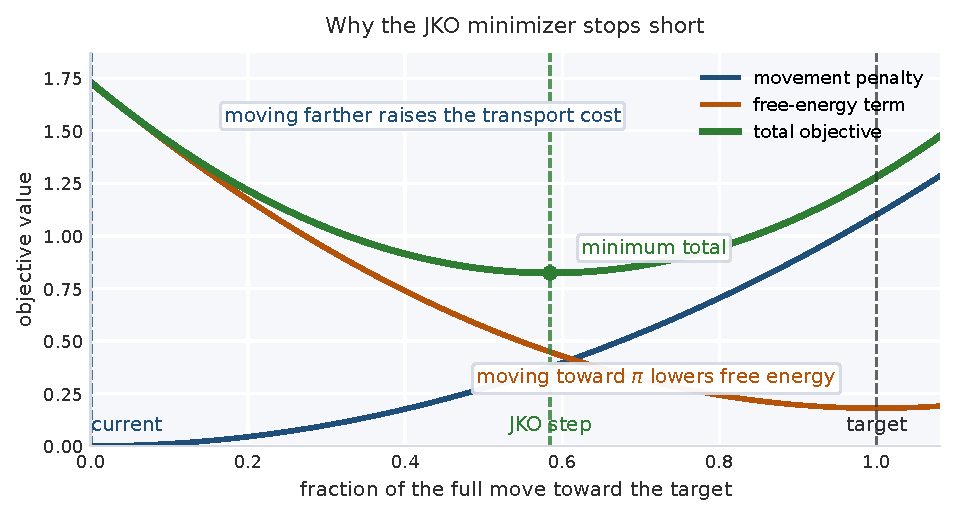
\includegraphics[width=0.9\linewidth]{figures/handouts/langevin_entropy_transport/fig_jko_tradeoff}
  \caption{One JKO step balances two competing effects.
  Moving farther toward equilibrium lowers the free-energy term, but it also increases the Wasserstein movement penalty, so the minimizer of the total objective stops at an interior compromise rather than jumping all the way to $\pi$.}
  \label{fig:jko-tradeoff}
\end{figure}

For a time step $h>0$, the JKO update is
\begin{equation}
  \rho_{k+1}
  \in
  \argmin_{\rho\in\mathcal{P}_2(\R^d)}
  \left\{
    \frac{1}{2h}W_2^2(\rho,\rho_k)+\mathcal{F}(\rho)
  \right\}.
  \label{eq:jko-step}
\end{equation}
The first term penalizes moving too far from the current density.
The second rewards lower free energy.
\Cref{fig:jko-tradeoff} is the picture to keep in mind: JKO is not ``jump to the minimizer of $\mathcal{F}$''; it is a one-step compromise between transport cost and dissipation.

\subsection{A Gaussian JKO calculation}
\label{subsec:jko-gaussian}

Take a quadratic target
\[
U(x)=\frac12 x^\top Hx,
\qquad
H\succ 0,
\]
so the equilibrium law is $\pi=\mathcal{N}(0,H^{-1})$.
To see what \eqref{eq:jko-step} is doing, first restrict attention to the translated Gaussian family
\[
\rho_m:=\mathcal{N}(m,H^{-1}),
\qquad
m\in\R^d.
\]
The covariance already matches the target, so only the mean is moving.

\begin{proposition}[Gaussian JKO mean update]
\label{prop:gaussian-jko-mean}
Fix $m_k\in\R^d$ and let $\rho_k=\rho_{m_k}$.
If we minimize the JKO objective \eqref{eq:jko-step} over translated Gaussians $\rho_m$, then
\begin{equation}
  m_{k+1}
  =
  (I_d+hH)^{-1}m_k.
  \label{eq:gaussian-jko-mean}
\end{equation}
Equivalently, the mean follows implicit Euler for the ODE $\dot m=-Hm$.
\end{proposition}

\begin{proof}
All densities $\rho_m$ have the same covariance, so their entropy terms are equal.
By \Cref{prop:free-energy-kl},
\[
\mathcal{F}(\rho_m)-\mathcal{F}(\pi)=D_{\mathrm{KL}}(\rho_m\|\pi).
\]
For Gaussians with common covariance $H^{-1}$,
\[
D_{\mathrm{KL}}(\rho_m\|\pi)=\frac12 m^\top Hm,
\qquad
W_2^2(\rho_m,\rho_{m_k})=\norm{m-m_k}_2^2.
\]
Therefore minimizing \eqref{eq:jko-step} over the translated family is exactly
\[
m_{k+1}
\in
\argmin_{m\in\R^d}
\left\{
\frac{1}{2h}\norm{m-m_k}_2^2+\frac12 m^\top Hm
\right\}.
\]
The first-order condition is
\[
\frac{1}{h}(m_{k+1}-m_k)+Hm_{k+1}=0,
\]
which rearranges to \eqref{eq:gaussian-jko-mean}.%
\end{proof}

This is already a real calculation, not a slogan.
JKO reproduces the correct mean evolution and it does so through an \emph{implicit} step.
That implicit character matters.
If $H=Q\Lambda Q^\top$ with $\Lambda=\mathrm{diag}(\lambda_1,\dots,\lambda_d)$ and $u_k:=Q^\top m_k$, then
\begin{equation}
  u_{k+1,i}
  =
  \frac{1}{1+h\lambda_i}\,u_{k,i},
  \qquad i=1,\dots,d.
  \label{eq:jko-modewise}
\end{equation}
Every mode contracts, and stiffer modes contract more aggressively.
There is no explicit-Euler stability restriction of the form $h<2/\lambda_{\max}$ in this mean calculation.
That is one reason minimizing movements are such a natural analytic tool.

\begin{figure}[t]
  \centering
  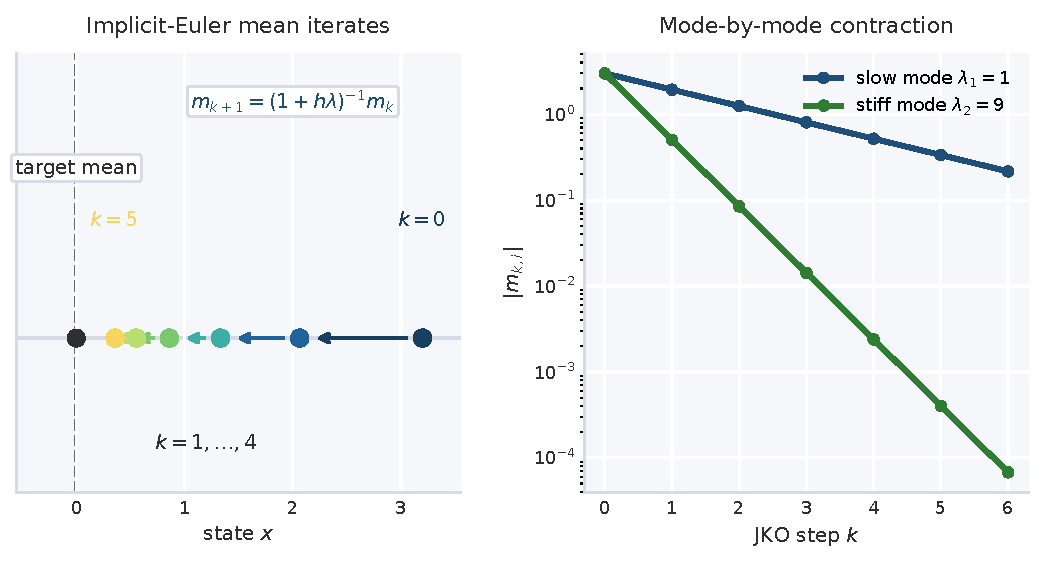
\includegraphics[width=0.9\linewidth]{figures/handouts/langevin_entropy_transport/fig_gaussian_jko_steps}
  \caption{For a quadratic target, restricting JKO to translated Gaussians keeps the covariance fixed and moves only the mean.
  That mean update is exactly implicit Euler, and in diagonal coordinates each mode contracts by $(1+h\lambda_i)^{-1}$, so stiff directions settle faster.}
  \label{fig:gaussian-jko}
\end{figure}

\Cref{fig:gaussian-jko} makes the same point visually.
The left panel shows the mean locations of those translated-Gaussian minimizers.
Because the covariance is fixed inside this restricted family, tracking the means is enough to see the entire update.
The right panel shows the mode-by-mode damping from \eqref{eq:jko-modewise}.

\begin{exercise}[Computing the Gaussian JKO mean step]
\label{ex:gaussian-jko-mean}
Work in the translated Gaussian family from \Cref{prop:gaussian-jko-mean}.
\begin{enumerate}[leftmargin=*]
  \item Show that $W_2^2(\rho_m,\rho_{m_k})=\norm{m-m_k}_2^2$.
  \item Show that $\mathcal{F}(\rho_m)-\mathcal{F}(\pi)=\tfrac12 m^\top Hm$.
  \item Derive \eqref{eq:gaussian-jko-mean} and the mode-by-mode contraction formula \eqref{eq:jko-modewise}.
\end{enumerate}
\end{exercise}
\SolutionBox[16]{%
\begin{enumerate}[leftmargin=*]
  \item Since $\rho_m$ and $\rho_{m_k}$ have the same covariance, the optimal transport is just translation by $m-m_k$, so
  \[
  W_2^2(\rho_m,\rho_{m_k})=\norm{m-m_k}_2^2.
  \]
  \item By \Cref{prop:free-energy-kl},
  \[
  \mathcal{F}(\rho_m)-\mathcal{F}(\pi)=D_{\mathrm{KL}}(\rho_m\|\pi).
  \]
  For Gaussians with equal covariance $H^{-1}$, the KL divergence reduces to the quadratic mean term
  \[
  D_{\mathrm{KL}}(\rho_m\|\pi)=\frac12 m^\top Hm.
  \]
  \item Therefore the JKO objective restricted to translated Gaussians is
  \[
  \Phi(m)=\frac{1}{2h}\norm{m-m_k}_2^2+\frac12 m^\top Hm.
  \]
  Its gradient is
  \[
  \nabla \Phi(m)=\frac{1}{h}(m-m_k)+Hm.
  \]
  Setting this to zero at the minimizer gives
  \[
  \frac{1}{h}(m_{k+1}-m_k)+Hm_{k+1}=0,
  \]
  hence
  \[
  m_{k+1}=(I_d+hH)^{-1}m_k.
  \]
  If $H=Q\Lambda Q^\top$ and $u_k=Q^\top m_k$, then
  \[
  u_{k+1}=Q^\top(I_d+hH)^{-1}Q\,u_k=(I_d+h\Lambda)^{-1}u_k,
  \]
  so each coordinate satisfies
  \[
  u_{k+1,i}=\frac{1}{1+h\lambda_i}u_{k,i}.
  \]
\end{enumerate}%
}

\subsection{The implicit velocity law}
\label{subsec:jko-velocity-law}

The mean calculation shows the basic mechanism in one tractable family, but the full measure-space update has an equally important first-order condition.
If $\rho_{k+1}$ is a smooth positive minimizer of \eqref{eq:jko-step} and $T_{k+1}$ is the optimal transport map from $\rho_{k+1}$ to $\rho_k$, then the Euler--Lagrange condition can be written as
\begin{equation}
  \frac{\operatorname{id}-T_{k+1}}{h}
  =
  -\nabla\bigl(U+\log \rho_{k+1}\bigr)
  \qquad \rho_{k+1}\text{-a.e.}
  \label{eq:jko-euler-lagrange}
\end{equation}
see \citet[\S4.5, Prop.~4.16]{santambrogio_2016_gradient_flows_overview}.
This is exactly the measure-space analogue of the implicit Euler equation
\[
\frac{x_{k+1}-x_k}{h}=-\nabla F(x_{k+1}).
\]
The transport displacement per unit time equals the free-energy velocity, evaluated at the \emph{new} density.

\subsection{The general JKO theorem}
\label{subsec:jko-general-theorem}

The full theorem is much deeper than the Gaussian example, and we do not try to reproduce the compactness proof here.
For our purposes, the conclusion is the key point.

\begin{theorem}[JKO scheme for Fokker--Planck, cited]
\label{thm:jko-general}
In the regular setting treated in \citet[\S4.5, Eq.~(4.13), Prop.~4.14, Prop.~4.19, pp.~37--42]{santambrogio_2016_gradient_flows_overview}, each minimization problem in \eqref{eq:jko-step} is well posed, and as $h\downarrow 0$ the recursive minimizers admit piecewise constant or geodesic interpolants that converge to the solution of the corresponding Fokker--Planck equation with the prescribed initial density.
In this sense, the Fokker--Planck equation is the $W_2$-gradient flow of free energy.
\end{theorem}

The cited proof is written on a compact domain with a $C^1$ confinement potential.
For the Langevin setting on $\R^d$, one imposes the corresponding confinement and integrability assumptions to recover the same minimizing-movement picture.
That theorem is the mathematical heart of the note.
It upgrades the formal continuity-equation picture from \Cref{prop:fokker-planck-continuity} into a precise variational statement: Langevin is not merely a diffusion with invariant law $\pi$; it is the steepest descent of $\mathcal{F}$ in Wasserstein geometry.
The right way to read the theorem is as an infinite-dimensional implicit-Euler convergence statement.
For each fixed $h$, the JKO rule produces a discrete descent path of densities.
As the step size shrinks, those variational steps converge to the actual Fokker--Planck evolution.
So the proximal picture is not just an analogy borrowed from optimization language; it is a literal construction of the PDE.

\section{An exact decay identity}
\label{sec:entropy-dissipation}

JKO identifies the geometry of the flow.
The next step is to compute an exact time derivative.
That is what turns the variational picture into a quantitative convergence argument.

\subsection{The instantaneous decay rate}
\label{subsec:fisher-dissipation}

The quantity that records this instantaneous decay rate is the \emph{relative Fisher information}.
It is defined by
\begin{equation}
  I(\rho\|\pi)
  :=
  \int_{\R^d}
  \norm{\nabla\log\frac{\rho}{\pi}}_2^2\,\rho\,dx.
  \label{eq:relative-fisher}
\end{equation}
Because $\log \pi=-U-\log Z$, this can also be written as
\[
I(\rho\|\pi)
=
\int \norm{\nabla(U+\log\rho)}_2^2\,\rho\,dx.
\]
It measures the squared size of the free-energy slope.

\begin{proposition}[Entropy dissipation identity]
\label{prop:entropy-dissipation}
Let $(\rho_t)_{t\ge 0}$ solve the Langevin Fokker--Planck equation.
Under the smoothness and decay assumptions needed for integration by parts,
\begin{equation}
  \frac{d}{dt}D_{\mathrm{KL}}(\rho_t\|\pi)
  =
  -I(\rho_t\|\pi).
  \label{eq:entropy-dissipation}
\end{equation}
\end{proposition}

\begin{proof}
Using mass conservation, $\int \partial_t \rho_t\,dx=0$, we may differentiate the entropy functional as
\begin{align*}
  \frac{d}{dt}D_{\mathrm{KL}}(\rho_t\|\pi)
  &=
  \int \log\frac{\rho_t}{\pi}\,\partial_t \rho_t\,dx.
\end{align*}
From \Cref{prop:fokker-planck-continuity},
\[
\partial_t \rho_t
=
\nabla\cdot\!\left(\rho_t\nabla\log\frac{\rho_t}{\pi}\right).
\]
Therefore
\begin{align*}
  \frac{d}{dt}D_{\mathrm{KL}}(\rho_t\|\pi)
  &=
  \int \log\frac{\rho_t}{\pi}
  \nabla\cdot\!\left(\rho_t\nabla\log\frac{\rho_t}{\pi}\right)\,dx \\
  &=
  -\int
  \norm{\nabla\log\frac{\rho_t}{\pi}}_2^2
  \rho_t\,dx \\
  &=
  -I(\rho_t\|\pi),
\end{align*}
which is \eqref{eq:entropy-dissipation}.%
\end{proof}

\Cref{prop:entropy-dissipation} is the exact dynamic counterpart of \Cref{prop:free-energy-kl}.
Relative entropy is the gap to equilibrium, and Fisher information is the instantaneous rate at which Langevin closes that gap.

\begin{exercise}[Deriving entropy dissipation]
\label{ex:entropy-dissipation}
Starting from \Cref{eq:fokker-planck-continuity}, prove \Cref{eq:entropy-dissipation}.
Then explain why $I(\rho_t\|\pi)=0$ forces $\rho_t=\pi$ under mild connectedness assumptions.
\end{exercise}
\SolutionBox[14]{%
We begin with
\[
D_{\mathrm{KL}}(\rho_t\|\pi)=\int \rho_t \log\frac{\rho_t}{\pi}\,dx.
\]
Since $\int \partial_t \rho_t\,dx=0$,
\[
\frac{d}{dt}D_{\mathrm{KL}}(\rho_t\|\pi)
=
\int \log\frac{\rho_t}{\pi}\,\partial_t \rho_t\,dx.
\]
Using the continuity-equation form,
\[
\partial_t \rho_t
=
\nabla\cdot\!\left(\rho_t\nabla\log\frac{\rho_t}{\pi}\right),
\]
we obtain
\begin{align*}
\frac{d}{dt}D_{\mathrm{KL}}(\rho_t\|\pi)
&=
\int \log\frac{\rho_t}{\pi}\,
\nabla\cdot\!\left(\rho_t\nabla\log\frac{\rho_t}{\pi}\right)\,dx \\
&=
-\int \norm{\nabla\log\frac{\rho_t}{\pi}}_2^2\,\rho_t\,dx \\
&=
-I(\rho_t\|\pi).
\end{align*}
If $I(\rho_t\|\pi)=0$, then $\nabla\log(\rho_t/\pi)=0$ almost everywhere on the support of $\rho_t$, so $\rho_t/\pi$ is constant on each connected component.
Both densities integrate to $1$, so that constant must be $1$, hence $\rho_t=\pi$ almost everywhere.%
}

\subsection{An exact Ornstein--Uhlenbeck example}
\label{subsec:ou-example}

The entropy dissipation identity is completely explicit for Gaussian targets.
Let
\[
U(x)=\frac12 x^\top Hx,
\qquad
H\succ 0,
\qquad
\pi=\mathcal{N}(0,H^{-1}).
\]
Suppose the initial law is
\[
\rho_0=\mathcal{N}(m_0,H^{-1}),
\]
so the covariance already matches equilibrium.
Then the Langevin diffusion preserves Gaussianity and only the mean moves:
\[
\rho_t=\mathcal{N}(m_t,H^{-1}),
\qquad
m_t=e^{-Ht}m_0.
\]
Writing $m_{0,i}$ in an eigenbasis of $H$ with eigenvalues $\lambda_i$ gives
\begin{equation}
  D_{\mathrm{KL}}(\rho_t\|\pi)
  =
  \frac12\sum_{i=1}^d \lambda_i m_{0,i}^2 e^{-2\lambda_i t},
  \qquad
  I(\rho_t\|\pi)
  =
  \sum_{i=1}^d \lambda_i^2 m_{0,i}^2 e^{-2\lambda_i t}.
  \label{eq:ou-kl-fisher}
\end{equation}
Differentiating the first display immediately yields
\[
\frac{d}{dt}D_{\mathrm{KL}}(\rho_t\|\pi)
=
-I(\rho_t\|\pi).
\]
This example is worth keeping in mind because every later result here collapses to an exact mode-by-mode statement in this quadratic setting.

\section{When decay becomes a uniform rate}
\label{sec:lsi}

Entropy dissipation by itself is only an identity.
It tells us the instantaneous decay rate,
\[
\frac{d}{dt}D_{\mathrm{KL}}(\rho_t\|\pi)=-I(\rho_t\|\pi),
\]
but not whether that rate is uniformly large when the chain is still far from equilibrium.
In principle the Fisher information could be small even while the entropy gap is still substantial.
To turn dissipation into a quantitative rate, we need an inequality that forces a large entropy gap to come with a large slope.
The standard tool is the log-Sobolev inequality, and the Bakry--\'Emery criterion is the curvature condition that often guarantees it.

\subsection{A functional inequality that closes the estimate}
\label{subsec:lsi-decay}

A log-Sobolev inequality compares the entropy gap directly to its dissipation.
Because
\[
I(\rho\|\pi)=\int \norm{\nabla \log(\rho/\pi)(x)}_2^2\,\rho(x)\,dx,
\]
the Fisher information is the squared $L^2(\rho)$ size of the relative log-density gradient.
Geometrically, it measures how sharply the density ratio $\rho/\pi$ is still tilted across space.
The log-Sobolev inequality says that a distribution cannot keep a large free-energy gap while that relative tilt is uniformly tiny.
Equivalently, a large mismatch from equilibrium must leave enough slope for Langevin to keep pushing downhill.

\begin{definition}[Log-Sobolev inequality]
\label{def:lsi}
We say that $\pi$ satisfies a log-Sobolev inequality with constant $\alpha>0$ if
\begin{equation}
  D_{\mathrm{KL}}(\rho\|\pi)
  \le
  \frac{1}{2\alpha}I(\rho\|\pi)
  \qquad
  \text{for every smooth density }\rho.
  \label{eq:lsi}
\end{equation}
\end{definition}

\begin{proposition}[LSI implies exponential KL decay]
\label{prop:lsi-kl-decay}
If $\pi$ satisfies \eqref{eq:lsi} with constant $\alpha>0$, then every sufficiently regular Langevin solution satisfies
\begin{equation}
  D_{\mathrm{KL}}(\rho_t\|\pi)
  \le
  e^{-2\alpha t}D_{\mathrm{KL}}(\rho_0\|\pi).
  \label{eq:kl-exponential-decay}
\end{equation}
\end{proposition}

\begin{proof}
By \Cref{prop:entropy-dissipation},
\[
\frac{d}{dt}D_{\mathrm{KL}}(\rho_t\|\pi)
=
-I(\rho_t\|\pi).
\]
Applying the log-Sobolev inequality at time $t$ gives
\[
I(\rho_t\|\pi)\ge 2\alpha D_{\mathrm{KL}}(\rho_t\|\pi),
\]
hence
\[
\frac{d}{dt}D_{\mathrm{KL}}(\rho_t\|\pi)
\le
-2\alpha D_{\mathrm{KL}}(\rho_t\|\pi).
\]
Gronwall's inequality yields \eqref{eq:kl-exponential-decay}.%
\end{proof}

This is the precise place where ``strong log-concavity implies quantitative mixing'' becomes a theorem.
Once Fisher information dominates entropy, the free-energy gap decays exponentially.
The geometric message is that under an LSI the target has no extended almost-flat directions in which a nonequilibrium density can hide.
If $\rho_t$ still differs substantially from $\pi$, then the relative log-density must still have noticeable slope, so the Fokker--Planck flow cannot stall prematurely.

\subsection{The Gaussian benchmark}
\label{subsec:gaussian-lsi}

For the Gaussian target
\[
\gamma_m(dx)\propto e^{-\frac{m}{2}\norm{x}_2^2}\,dx,
\]
the correct LSI constant is $\alpha=m$.
One way to see that is to invoke the curvature criterion in the next subsection, since $\Hess U=mI_d$.
Inside the translated Gaussian family, the constant is visible exactly:
if $\rho=\mathcal{N}(a,m^{-1}I_d)$, then
\[
D_{\mathrm{KL}}(\rho\|\gamma_m)=\frac{m}{2}\norm{a}_2^2,
\qquad
I(\rho\|\gamma_m)=m^2\norm{a}_2^2,
\]
so equality holds in \eqref{eq:lsi}.
That is a useful sanity check.
The Gaussian measure is not merely an example where LSI is true; it is the model case where the constants are exact.

\subsection{Curvature gives LSI}
\label{subsec:bakry-emery}

The next question is where a bound like \eqref{eq:lsi} comes from.
For strongly log-concave targets, the answer is curvature.
If $U$ bends upward everywhere by at least a fixed quadratic amount, then the measure has no broad flat directions in which entropy can stay large while the free-energy slope becomes tiny.
The Bakry--\'Emery criterion turns that idea into a global log-Sobolev constant.

\begin{theorem}[Bakry--\'Emery criterion, cited]
\label{thm:bakry-emery}
Let $\pi(dx)=Z^{-1}e^{-U(x)}\,dx$ on $\R^d$, where $U\in C^2(\R^d)$ and $Z<\infty$.
If
\begin{equation}
  \Hess U(x)\succeq mI_d
  \qquad\text{for every }x\in\R^d
  \label{eq:bakry-emery-curvature}
\end{equation}
for some $m>0$, then $\pi$ satisfies a log-Sobolev inequality with constant $\alpha=m$.
\end{theorem}

We cite \citet[Thm.~2]{otto_villani_2000_talagrand_lsi} for this form of the theorem.
Historically it is the Bakry--\'Emery curvature condition.
The proof uses $\Gamma_2$-calculus rather than the transport arguments used in the surrounding development, so we do not reproduce it.

The geometric meaning of \eqref{eq:bakry-emery-curvature} is that the ambient space always looks at least as confining as a quadratic well.
If $U$ has a uniform quadratic lower bound on curvature, then the target has no flat directions that allow entropy to linger and no broad corridors in which mass can drift with only a weak restoring force.
Misplaced mass must create a visible change in the relative log-density, so the free-energy slope cannot be tiny unless the entropy gap is already small.
That is exactly what \eqref{eq:lsi} formalizes.
What makes the theorem powerful is that it is global.
The lower Hessian bound is required at every point, not just near the mode, and the conclusion controls every smooth density $\rho$.
One can think of $m$ as a universal restoring-force constant: no matter where mass moves, the landscape is always at least as curved as a quadratic well of curvature $m$.
Bakry--\'Emery says that this geometric fact is enough to force a uniform entropy-dissipation estimate.

\section{From entropy to transport}
\label{sec:entropy-to-transport}

We now have an exponential decay theorem in KL divergence.
For proving convergence, that is already enough.
The reason to keep going is that KL and Wasserstein distance answer different questions.
The KL divergence measures excess free energy, while $W_2$ measures how far the mass of $\rho_t$ still has to move in space to match $\pi$.
That geometric viewpoint is closer to the coupling language of the Sampling unit and the conditioning language of the Optimization unit, so it is worth translating entropy control into transport control as well.

\begin{definition}[Talagrand's $T_2$ inequality]
\label{def:t2}
We say that $\pi$ satisfies $T_2(\alpha)$ if
\begin{equation}
  W_2^2(\rho,\pi)
  \le
  \frac{2}{\alpha}D_{\mathrm{KL}}(\rho\|\pi)
  \qquad
  \text{for every density }\rho.
  \label{eq:t2}
\end{equation}
\end{definition}

\begin{theorem}[Otto--Villani, cited]
\label{thm:otto-villani}
Let $\pi(dx)=Z^{-1}e^{-U(x)}\,dx$ be a probability measure on $\R^d$ with finite second moment, where $U\in C^2(\R^d)$ and
\[
\Hess U(x)\succeq C I_d
\qquad\text{for every }x\in\R^d
\]
for some $C\in\R$.
If $\pi$ satisfies a log-Sobolev inequality with constant $\alpha>0$, then $\pi$ also satisfies $T_2(\alpha)$.
\end{theorem}

This is \citet[Thm.~1]{otto_villani_2000_talagrand_lsi}.
It says that once entropy is controlled, the amount of spatial transport still needed to reach equilibrium is controlled automatically.
That is not obvious a priori because the two quantities measure different kinds of mismatch.
The KL divergence compares density values pointwise, while $W_2$ measures the cost of rearranging mass in space.
The theorem says that an LSI is strong enough to connect them: under sufficient curvature, any large remaining transport cost would itself force a large entropy gap.
So transport control is not an extra ingredient added on top of entropy control; it is a geometric consequence of the same inequality.

\begin{samepage}
\begin{corollary}[Wasserstein decay from LSI]
\label{cor:wasserstein-decay}
Under the hypotheses of \Cref{thm:otto-villani}, every sufficiently regular Langevin solution satisfies
\begin{equation}
  W_2(\rho_t,\pi)
  \le
  \sqrt{\frac{2}{\alpha}}\,
  e^{-\alpha t}
  \sqrt{D_{\mathrm{KL}}(\rho_0\|\pi)}.
  \label{eq:w2-decay}
\end{equation}
\end{corollary}
\end{samepage}

\begin{proof}
Combine \Cref{thm:otto-villani} with \Cref{prop:lsi-kl-decay}:
\[
W_2^2(\rho_t,\pi)
\le
\frac{2}{\alpha}D_{\mathrm{KL}}(\rho_t\|\pi)
\le
\frac{2}{\alpha}e^{-2\alpha t}D_{\mathrm{KL}}(\rho_0\|\pi).
\]
Taking square roots gives \eqref{eq:w2-decay}.%
\end{proof}

For the Gaussian family from \Cref{subsec:gaussian-lsi}, the bridge is exact on translated states:
if $\rho=\mathcal{N}(a,m^{-1}I_d)$ and $\gamma_m=\mathcal{N}(0,m^{-1}I_d)$, then
\[
W_2^2(\rho,\gamma_m)=\norm{a}_2^2=\frac{2}{m}D_{\mathrm{KL}}(\rho\|\gamma_m).
\]
So the LSI-to-$T_2$ story is not merely qualitative.
Its constants are already sharp in the Gaussian model.

\begin{exercise}[From LSI to a Wasserstein bound]
\label{ex:lsi-to-w2}
Assume $\pi$ satisfies LSI$(\alpha)$.
\begin{enumerate}[leftmargin=*]
  \item Use \Cref{prop:entropy-dissipation} to derive \Cref{eq:kl-exponential-decay}.
  \item Combine that with \Cref{eq:t2} to prove \Cref{eq:w2-decay}.
  \item Verify directly in the translated Gaussian family that $T_2(\alpha)$ holds with equality.
\end{enumerate}
\end{exercise}
\SolutionBox[14]{%
\begin{enumerate}[leftmargin=*]
  \item By entropy dissipation,
  \[
  \frac{d}{dt}D_{\mathrm{KL}}(\rho_t\|\pi)=-I(\rho_t\|\pi).
  \]
  The LSI bound gives
  \[
  I(\rho_t\|\pi)\ge 2\alpha D_{\mathrm{KL}}(\rho_t\|\pi),
  \]
  so
  \[
  \frac{d}{dt}D_{\mathrm{KL}}(\rho_t\|\pi)\le -2\alpha D_{\mathrm{KL}}(\rho_t\|\pi).
  \]
  Gronwall yields
  \[
  D_{\mathrm{KL}}(\rho_t\|\pi)\le e^{-2\alpha t}D_{\mathrm{KL}}(\rho_0\|\pi).
  \]
  \item Talagrand's inequality gives
  \[
  W_2^2(\rho_t,\pi)\le \frac{2}{\alpha}D_{\mathrm{KL}}(\rho_t\|\pi).
  \]
  Substituting the KL decay bound,
  \[
  W_2^2(\rho_t,\pi)\le \frac{2}{\alpha}e^{-2\alpha t}D_{\mathrm{KL}}(\rho_0\|\pi),
  \]
  and taking square roots gives \eqref{eq:w2-decay}.
  \item For $\gamma_\alpha=\mathcal{N}(0,\alpha^{-1}I_d)$ and $\rho=\mathcal{N}(a,\alpha^{-1}I_d)$,
  \[
  W_2^2(\rho,\gamma_\alpha)=\norm{a}_2^2
  \]
  because the optimal transport is translation by $a$, while
  \[
  D_{\mathrm{KL}}(\rho\|\gamma_\alpha)=\frac{\alpha}{2}\norm{a}_2^2.
  \]
  Hence
  \[
  W_2^2(\rho,\gamma_\alpha)=\frac{2}{\alpha}D_{\mathrm{KL}}(\rho\|\gamma_\alpha),
  \]
  so $T_2(\alpha)$ is attained exactly on this translated Gaussian family.%
\end{enumerate}
}

\section{Preconditioning and a real posterior}
\label{sec:preconditioning-real-data}

The functional-inequality chain explains why Langevin converges.
The final question is where the constants come from in practice.
For quadratic or locally quadratic targets, the answer is geometric: the relevant rates are the eigenvalues of the preconditioned Hessian.

\subsection{Quadratic targets and the rate matrix}
\label{subsec:preconditioning-quadratic}

Now return to geometry.
Consider the preconditioned overdamped Langevin diffusion
\begin{equation}
  dX_t=-M\nabla U(X_t)\,dt+\sqrt{2M}\,dB_t,
  \label{eq:preconditioned-langevin}
\end{equation}
where $M\succ 0$ is a fixed symmetric positive-definite matrix.
For a quadratic potential centered at $x_\star$,
\[
U(x)=\frac12 (x-x_\star)^\top H(x-x_\star),
\qquad
H\succ 0,
\]
the geometry is again exact.

\begin{proposition}[The relevant rate matrix is $M^{1/2}HM^{1/2}$]
\label{prop:preconditioned-rate-matrix}
Let $Y_t:=M^{-1/2}(X_t-x_\star)$.
Then \eqref{eq:preconditioned-langevin} becomes
\begin{equation}
  dY_t=-A Y_t\,dt+\sqrt{2}\,dB_t,
  \qquad
  A:=M^{1/2}HM^{1/2}.
  \label{eq:preconditioned-ou}
\end{equation}
Hence the mode-by-mode decay rates are the eigenvalues of $A$, not of $H$ alone.
In particular, if $M=H^{-1}$, then $A=I_d$ and all local modes are equalized.
\end{proposition}

\begin{proof}
Write $X_t=x_\star+M^{1/2}Y_t$.
Then
\[
dX_t=M^{1/2}dY_t,
\qquad
\nabla U(X_t)=H(X_t-x_\star)=HM^{1/2}Y_t.
\]
Substituting into \eqref{eq:preconditioned-langevin},
\[
M^{1/2}dY_t=-MHM^{1/2}Y_t\,dt+\sqrt{2M}\,dB_t.
\]
Multiplying by $M^{-1/2}$ gives
\[
dY_t=-M^{1/2}HM^{1/2}Y_t\,dt+\sqrt{2}\,dB_t,
\]
which is \eqref{eq:preconditioned-ou}.%
\end{proof}

The local conclusion is immediate.
Whitening is not mysterious.
It is exactly the choice of $M$ that turns the local quadratic surrogate into an isotropic Ornstein--Uhlenbeck process.

The entropy and transport quantities from earlier sections are also explicit here.
If the transformed process starts from
\[
Y_0\sim \mathcal{N}(m_0,A^{-1}),
\]
then
\[
Y_t\sim \mathcal{N}(e^{-At}m_0,A^{-1}),
\]
so in an eigenbasis of $A$ with eigenvalues $\nu_i$ and coordinates $c_i$ of $m_0$,
\begin{equation}
  D_{\mathrm{KL}}(\rho_t\|\pi)
  =
  \frac12\sum_i \nu_i c_i^2 e^{-2\nu_i t},
  \qquad
  I(\rho_t\|\pi)
  =
  \sum_i \nu_i^2 c_i^2 e^{-2\nu_i t},
  \qquad
  W_2^2(\rho_t,\pi)
  =
  \sum_i c_i^2 e^{-2\nu_i t}.
  \label{eq:preconditioned-decay-formulas}
\end{equation}
When $M=H^{-1}$, all $\nu_i$ become $1$, so every mode decays on the same time scale.

\begin{figure}[t]
  \centering
  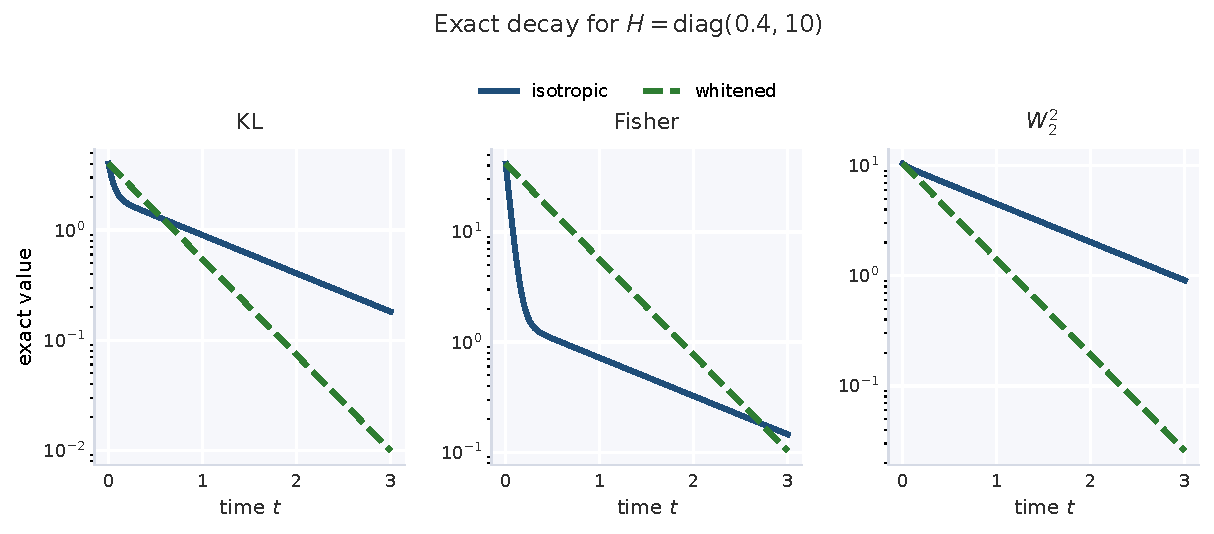
\includegraphics[width=0.95\linewidth]{figures/handouts/langevin_entropy_transport/fig_gaussian_decay_preconditioning}
  \caption{For an anisotropic Gaussian target, KL, Fisher information, and $W_2^2$ decay exactly under the local Ornstein--Uhlenbeck dynamics.
  Whitening turns the rate matrix into the identity and removes the slow mode.}
  \label{fig:gaussian-preconditioning}
\end{figure}

\Cref{fig:gaussian-preconditioning} shows \eqref{eq:preconditioned-decay-formulas} for a simple two-dimensional quadratic target.
The visual simplification reflects an analytic one.
Whitening changes the exact exponents appearing in every convergence quantity derived above.

\subsection{Bayesian logistic regression on the Problem Set 2 data}
\label{subsec:logistic-real-data}

To keep the real-data example aligned with the notes, we return to the regularized logistic-regression model that runs through the Optimization unit and reappears in Problem Set~2.
The dataset has five predictors and a binary response.
In the optimization material, this model supplied explicit gradients, Hessians, and the MAP/Laplace calculation.
Here the same local quadratic surrogate serves a different purpose: it reveals the local rate matrix seen by overdamped Langevin near the MAP.

Write
\[
\beta=(\beta_0,\beta_1,\dots,\beta_5)^\top,
\qquad
\tilde x_i=(1,x_{i1},\dots,x_{i5})^\top.
\]
We also keep the same isotropic Gaussian prior as in Problem Set~2,
\[
\beta\sim \mathcal{N}(0,100 I_6),
\]
so the prior precision is $\lambda=0.01$.
The negative log posterior is
\begin{equation}
  U(\beta)
  =
  \sum_{i=1}^n \Bigl[\log\!\bigl(1+e^{\tilde x_i^\top\beta}\bigr)-y_i \tilde x_i^\top\beta\Bigr]
  +
  \frac{\lambda}{2}\norm{\beta}_2^2.
  \label{eq:logistic-posterior}
\end{equation}
If $p_i(\beta)=\sigma(\tilde x_i^\top\beta)$ with $\sigma(t)=1/(1+e^{-t})$, then
\[
\nabla U(\beta)=X^\top(p(\beta)-y)+\lambda\beta,
\qquad
\Hess U(\beta)=X^\top W(\beta)X+\lambda I_6,
\]
where $W(\beta)$ is diagonal with entries $p_i(\beta)(1-p_i(\beta))$.

We compute the MAP estimate $\beta_{\mathrm{MAP}}$ numerically and use the Hessian
\[
H_{\mathrm{MAP}}:=\Hess U(\beta_{\mathrm{MAP}})
\]
as a local Gaussian surrogate.
This is exactly the Laplace approximation, and we use it only locally.
The claim is not that the posterior is globally Gaussian.
The claim is that the Hessian near the MAP reveals which local preconditioner equalizes the quadratic surrogate.

\begin{figure}[t]
  \centering
  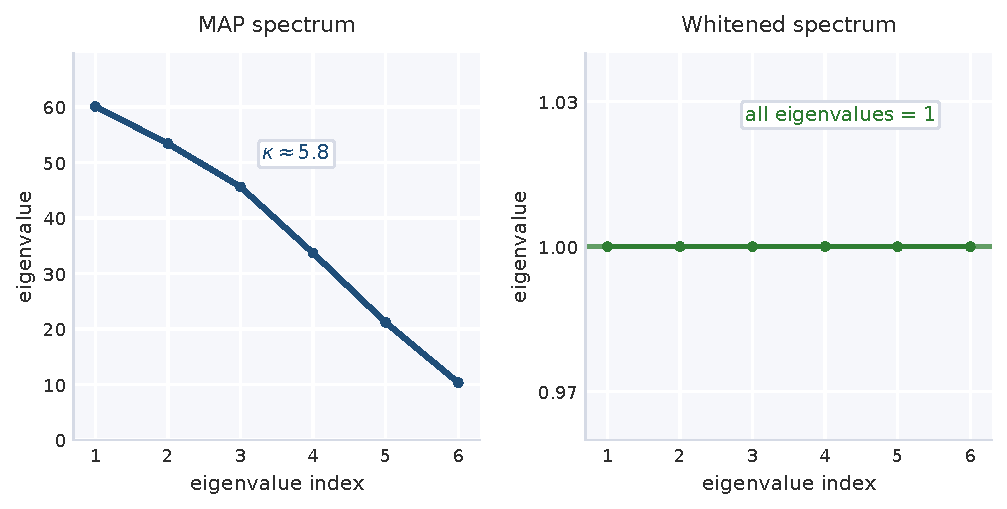
\includegraphics[width=0.92\linewidth]{figures/handouts/langevin_entropy_transport/fig_logistic_hessian_spectrum}
  \caption{The Problem Set 2 Bayesian logistic posterior has a nontrivial MAP Hessian spectrum.
  Whitening with $H_{\mathrm{MAP}}^{-1/2}$ collapses the local spectrum to $1$.}
  \label{fig:logistic-spectrum}
\end{figure}

\Cref{fig:logistic-spectrum} shows the full Hessian spectrum.
The raw local condition number is about $5.8$.
That is not extreme, but it is large enough to make the soft/stiff splitting visible in a familiar course example.
That spectrum is the continuous-time Langevin analogue of the conditioning language from the Optimization unit and the Sampling unit's gradient-based MCMC subsection.

\begin{figure}[t]
  \centering
  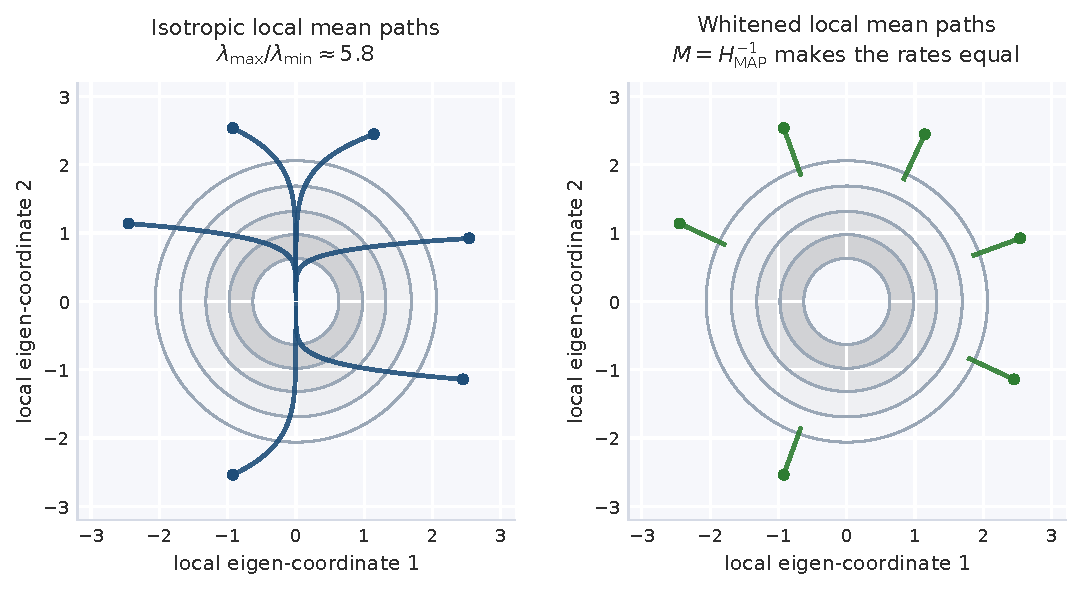
\includegraphics[width=0.92\linewidth]{figures/handouts/langevin_entropy_transport/fig_logistic_laplace_trajectories}
  \caption{The softest/stiffest eigenspace of the Laplace surrogate around the MAP.
  Without preconditioning, local mean paths pinch first along the stiff direction and only later move along the soft direction; local whitening equalizes the contraction rates.}
  \label{fig:logistic-trajectories}
\end{figure}

\Cref{fig:logistic-trajectories} turns the spectrum into a local picture.
Because this model has only six parameters, the figure uses the softest and stiffest eigendirections directly.
The message is the same in either case.
Without preconditioning, the local mean paths collapse first in the stiff direction while progress in the soft direction lags behind.
With $M=H_{\mathrm{MAP}}^{-1}$, the local quadratic surrogate has balanced rates.

This is the right closing connection to the course's conditioning language.
For overdamped Langevin, preconditioning changes the exact rate matrix controlling entropy dissipation and transport contraction.
The same local Hessian picture is what later makes mass-matrix choices matter in the Augmented-state sampling unit's HMC/NUTS development.

\begin{exercise}[Reading the local Hessian geometry]
\label{ex:logistic-preconditioner}
Use \Cref{prop:preconditioned-rate-matrix}, \Cref{fig:logistic-spectrum}, and \Cref{fig:logistic-trajectories}.
\begin{enumerate}[leftmargin=*]
  \item Explain why a spread in the eigenvalues of $H_{\mathrm{MAP}}$ produces multiple local mixing time scales for isotropic Langevin.
  \item Show that choosing $M=H_{\mathrm{MAP}}^{-1}$ makes the local rate matrix equal to the identity.
  \item Why is $H_{\mathrm{MAP}}^{-1}$ the natural quadratic preconditioner, up to an overall scalar factor?
\end{enumerate}
\end{exercise}
\SolutionBox[14]{%
\begin{enumerate}[leftmargin=*]
  \item In the quadratic surrogate, isotropic Langevin corresponds to $M=I_d$, so the local rate matrix is just $H_{\mathrm{MAP}}$.
  Its eigenvalues are the mode-by-mode contraction rates.
  If those eigenvalues vary widely, some directions equilibrate quickly while others remain slow, creating multiple local time scales.
  \item By \Cref{prop:preconditioned-rate-matrix},
  \[
  A=M^{1/2}H_{\mathrm{MAP}}M^{1/2}.
  \]
  Setting $M=H_{\mathrm{MAP}}^{-1}$ gives
  \[
  A=H_{\mathrm{MAP}}^{-1/2}H_{\mathrm{MAP}}H_{\mathrm{MAP}}^{-1/2}=I_d.
  \]
  So all local contraction rates become $1$.
  \item If the goal is to equalize the quadratic modes, then we want $A$ to be proportional to the identity.
  That means
  \[
  M^{1/2}H_{\mathrm{MAP}}M^{1/2}=cI_d
  \]
  for some scalar $c>0$, which is equivalent to
  \[
  M=c\,H_{\mathrm{MAP}}^{-1}.
  \]
  Thus $H_{\mathrm{MAP}}^{-1}$ is the natural local quadratic preconditioner, with any extra scalar factor only changing the overall time scale.%
\end{enumerate}
}

There is also a discrete-time algorithmic payoff.
Once one has an LSI and enough smoothness, these continuous-time decay arguments feed directly into nonasymptotic ULA theory; see \citet[\S3.1, Thm.~1]{vempala_wibisono_2019_ula_isoperimetry}.
The point of that cited result is not that Euler discretization exactly preserves the diffusion analysis.
Rather, good continuous-time geometry survives discretization up to a controlled error, so the same inequalities lead to quantitative bounds for an actual algorithm.
The course-level synthesis is now clear.
Free energy is the Lyapunov functional, JKO is the proximal structure, Fisher information supplies dissipation, LSI turns dissipation into a uniform rate, Talagrand converts that rate into transport control, and preconditioning changes the constants by changing the local geometry.
Carried back to the main notes, this is the optimization story returning in measure space: descent becomes entropy dissipation, proximal structure becomes JKO, and conditioning still determines which directions are easy and which are slow.

\bibliographystyle{plainnat}
\makeatletter
\begingroup
\let\input@path\@empty
\IfFileExists{references.bib}{%
  \gdef\stat221bibpath{references}%
}{%
  \IfFileExists{../references.bib}{%
    \gdef\stat221bibpath{../references}%
  }{%
    \gdef\stat221bibpath{../../references}%
  }%
}
\endgroup
\makeatother
\bibliography{\stat221bibpath}

\end{document}
